\chapter{ANIMAL DETECTION PIPELINE} \label{chapter:detection}

\noindent This chapter presents a pipeline of modular machine learning components that detect, classify, and otherwise prepare images of animals for use in a visual identification (ID) procedure.  The computer vision task of object detection includes the inherent step of finding animals in images but, when used as a prerequisite for animal ID, it needs to be able to do much more than just that.  For example, animal detection needs to determine an animal's species and viewpoint so that automated tools consider only annotations that can actually be compared; having ecological metadata like species and viewpoint increases the accuracy and speed of ID by filtering out annotations that could only function as potential confusers.  An annotation may also need to be rotated to allow accurate matching or have its background segmented out because it is distracting for algorithms or humans.  What is needed is a comprehensive pipeline that can perform a variety of different ``animal detection'' tasks so that an automated ID process can focus on its tasks of describing, retrieving, ranking, and verifying potential matches of animals.\blfootnote{Portions of this chapter previously appeared as: J. Parham and C. Stewart, ``Detecting plains and Grevy’s zebras in the real world,'' in \textit{IEEE Winter Conf. Applicat. Comput. Vis. Workshops}, Lake Placid, NY, USA, Mar. 2016, pp. 1–9.}\blfootnote{Portions of this chapter previously appeared as: J. Parham \textit{et al.}, ``An animal detection pipeline for identification,'' in \textit{IEEE Winter Conf. Applicat. Comput. Vis.}, Lake Tahoe, CA, USA, Mar. 2018, pp. 1–9.}

The animal detection problem can be exceedingly complex: there may be multiple (or no) animals from several different species in an image, some species might not be the target of ID but have a similar visual appearance to the species of interest, some annotations may have poor quality while others may show only parts of the animal, or an animal may be occluded by other animals or vegetation.  Furthermore, animals may be seen from various scales, viewpoints, and poses, only some showing identifiable information.  The images provided to the detection pipeline may also originate from handheld cameras used by trained ecologists or novices (e.g., tourists, children) with no prior experience taking photos of animals for photographic ID.  Images can also be captured by passive collection devices like a camera-trap or an aerial surveying platform.  The detection pipeline must account for these challenges and automate the creation of high-quality annotations useful for animal ID or wide-area aerial counts.

\begin{figure}[!t]
    \begin{center}
        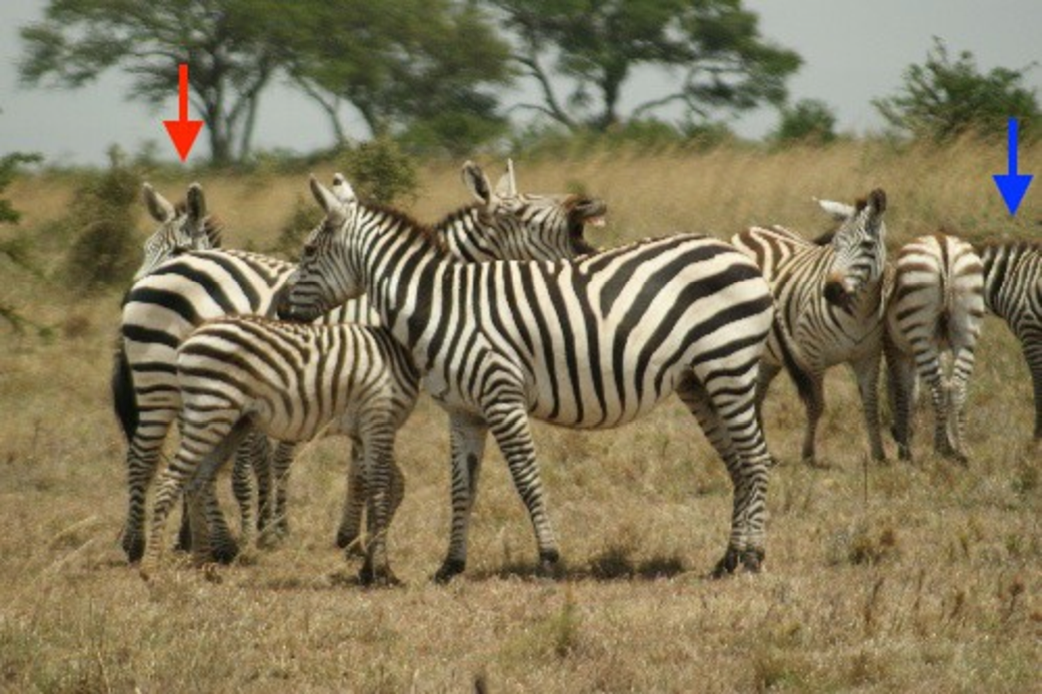
\includegraphics[width=0.80\linewidth]{resources/sample2-arrows.pdf}
    \end{center}
    \caption{The challenges of the detection problem (shown for plains zebras) include varying viewpoints, natural and artificial (image frame) occlusions, and overlapping animals.  The image shows 7 individual zebras with 5 differing viewpoints and 5 occlusions of differing severity.  The highlighted animals are almost completely occluded, but still clearly discernible.  \copyright 2016 IEEE. Reprinted, with permission, from: J. Parham and C. Stewart, ``Detecting plains and Grevy’s zebras in the real world,'' in \textit{IEEE Winter Conf. Applicat. Comput. Vis. Workshops}, Lake Placid, NY, USA, Mar. 2016, pp. 1–9.}
    \label{fig:challenge}
\end{figure}

The detection problem as applied to photographs of zebras, for example, has several real-world challenges: varying viewpoints, natural and artificial occlusions, overlapping animals (i.e., instinctual herding behavior), non-rigid body structures (legs, necks), and significant changes in visual appearance (e.g., genetic variations, dust, scarring).  Looking at Figure~\ref{fig:challenge}, the head of the highlighted zebra (red arrow) is visible, but the rest of the animal is almost completely occluded except for one or two legs.  The cut-off animal on the far right (blue arrow) only has a small section of neck visible, whereas its neighbor to the left is facing entirely away from the camera.  While the challenges listed above are not unique to zebras, they are typical for species that assemble in herds and social groups.  Zebras seen in the real world can be frustratingly uncooperative with respect to the task of trying to detect and identify them, which makes them an ideal challenge species for evaluation.  Furthermore, these kinds of challenging detection scenarios elevate the problem to a degree of difficulty not often seen in standard computer vision benchmarking competitions like PASCAL VOC~\cite{everingham_pascal_2010} and ILSVRC~\cite{russakovsky_imagenet_2015}.

\begin{figure}[!t]
    \begin{center}
        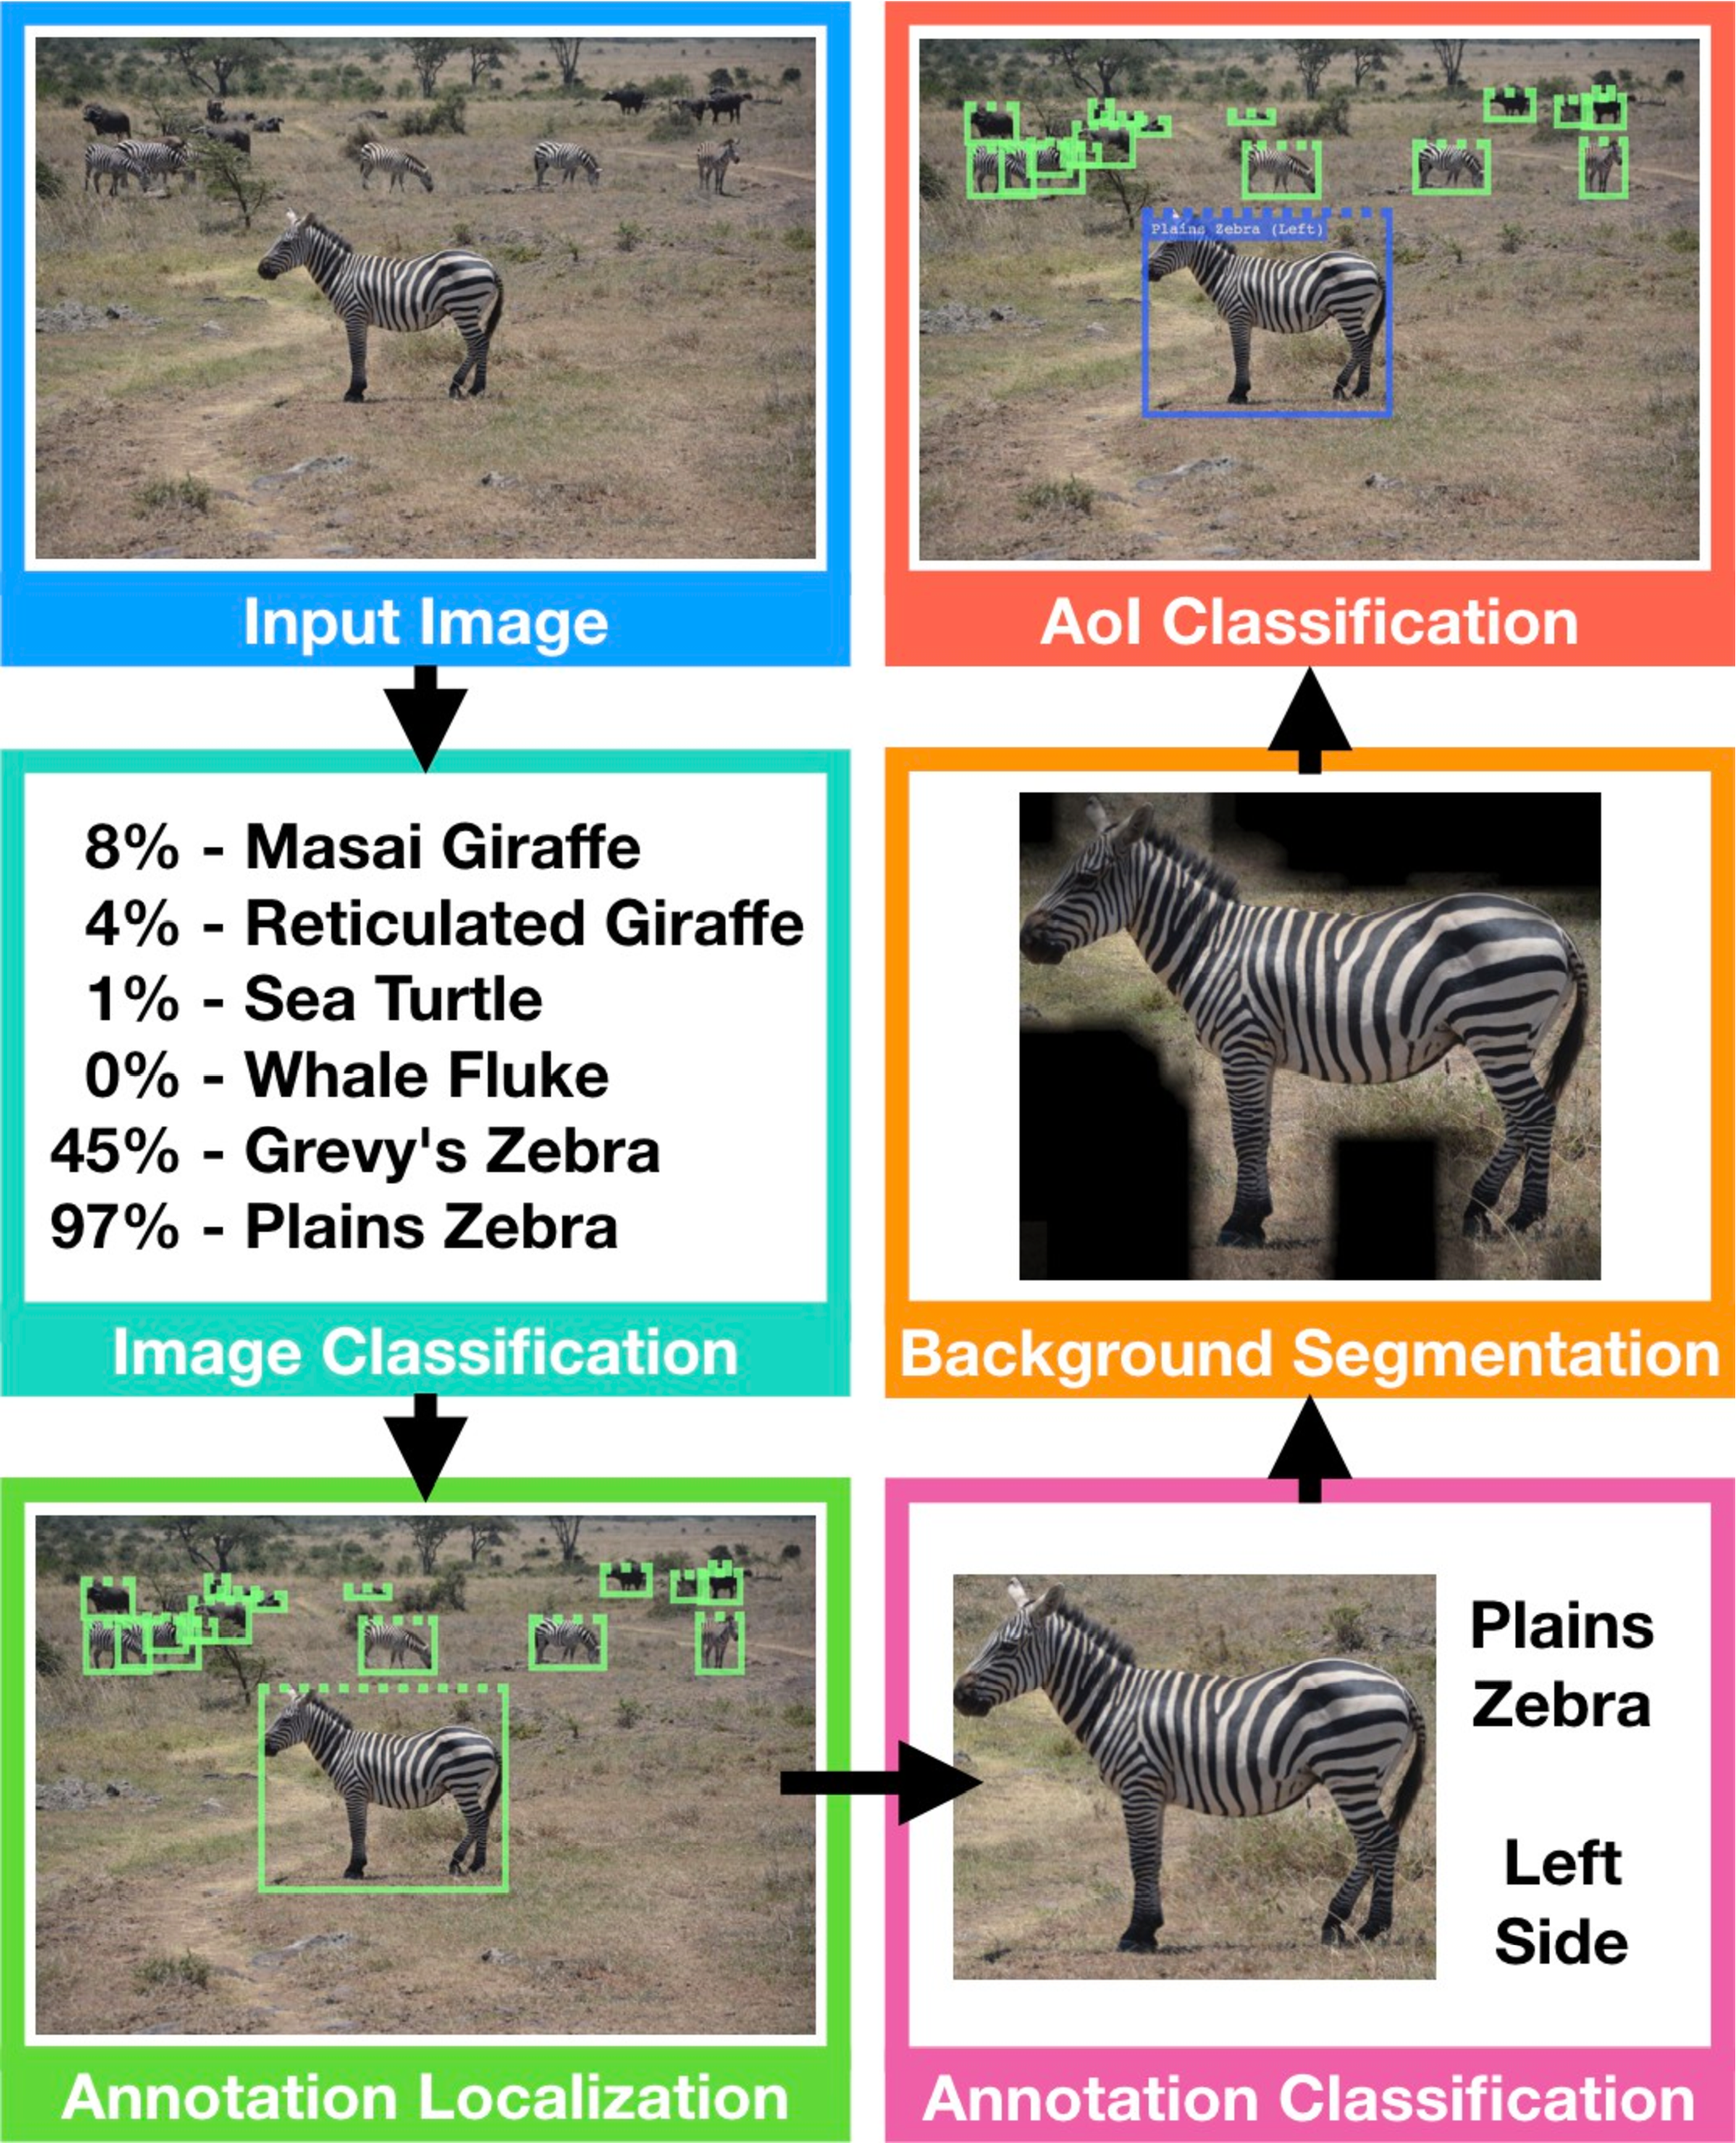
\includegraphics[width=0.8\linewidth]{resources/pipeline.pdf}
    \end{center}
    \caption{An overview of the detection pipeline and its components: 1) image classification provides a score for the species that exist in the image, 2) annotation localization places bounding boxes over the animals, 3) annotation classification adds species and viewpoint labels to each annotation, 4) annotation background segmentation computes a species-specific foreground-background mask, and 5) Annotation of Interest (AoI) classification predicts primary animal(s) of the image.  \copyright 2018 IEEE. Reprinted, with permission, from: J. Parham \textit{et al.}, ``An animal detection pipeline for identification,'' in \textit{IEEE Winter Conf. Applicat. Comput. Vis.}, Lake Tahoe, CA, USA, Mar. 2018, pp. 1–9.}
    \label{fig:pipeline}
\end{figure}

In response to the challenges outlined above, a five-component detection pipeline is proposed and analyzed in this chapter (see Figure~\ref{fig:pipeline} on the next page).  These components are, in order of their intended usage in the detection pipeline, the following: 1) whole-image classification to select the images that contain desired species or are otherwise relevant to the analysis, 2) bounding-box localization to form annotations, 3) annotation labeler to predict the animal's species and viewpoint, 4) coarse annotation segmentation to eliminate irrelevant background information, and 5) a classifier to select the ``Annotation(s) of Interest'' as the most prominent animal(s) in the image.  We will also discuss additional components and use cases that add functionality and make the detection pipeline a more comprehensive solution, including detecting parts within an annotation or orienting annotations with a predicted rotation.  We will start the discussion by reviewing two new datasets for animal detection that this research contributes.

\section{Animal Detection Datasets: WILD \& DETECT}

This chapter presents two new detection datasets, called WILD (Wildlife Images and Localizations Dataset) and DETECT, alongside the proposed detection pipeline.  The purpose of these datasets is to provide a more realistic collection of \textit{in situ} animal sightings that often are not found in public detection datasets.  The hope is that these datasets can motivate future ecological research on animal detection and provide examples of how best to curate datasets for the problem domain of animal re-ID.

\subsection{WILD Dataset}

The WILD dataset is comprised of photographs taken by biologists, wildlife rangers, citizen scientists~\cite{irwin_citizen_1995}, and conservationists, and captures detection scenarios that are uncommon in publicly-available computer vision datasets like PASCAL~\cite{everingham_pascal_2010}, ILSVRC~\cite{russakovsky_imagenet_2015}, and COCO~\cite{lin_microsoft_2014}.  Furthermore, human photographers implicitly curated all animal sightings in the WILD dataset (i.e., a person actively decided to take the picture).  This feature is in contrast to what would be seen in 1) movement-based camera trap, 2) exemplar-based datasets like iNaturalist\footnote{\url{inaturalist.org} (Accessed: Oct. 29, 2021).}, or 3) ``always-on'' overhead aerial surveys of animals.  Unfortunately, most computer vision datasets make no distinction between wild animal sightings and other representations of that species (e.g., a stuffed zebra animal toy or animals seen only in captivity).  Public challenge datasets are not representative of the types of images generally collected by park rangers and tourists, which is how image data for animal population censusing is gathered (discussed in Chapter~\ref{chapter:censusing}).  Class definitions that allow broad acceptance distract from the task of detecting real-world sightings of animals in the wild and are generally incompatible with ID.  In contrast, all of the images in the WILD dataset were taken of wild animals in their natural habitats.

The species cataloged by WILD are 1) Masai giraffe (\textit{Giraffa camelopardalis tippelskirchi}), 2) reticulated giraffe (\textit{Giraffa reticulata}), 3) sea turtle (\textit{Chelonia mydas} and \textit{Eretmochelys imbricata}), 4) humpback whale fluke (above-water flukes of \textit{Megaptera novaeangliae}), 5) Gr\'evy's zebra (\textit{Equus grevyi}), and 6) plains zebra (\textit{Equus quagga}).  The WILD dataset offers challenging detection scenarios for each species; for example, zebras and giraffes tend to form social groups and stand close together, creating sightings with frequent bounding box overlap, occlusion, and cross-species co-location.  It would be hard, or at the very least inefficient, to capture this level of complexity in artificial settings like a zoo -- especially since a zoo setting largely omits the chance of seeing other species in the same image and will duplicate background textures.  The common practice for sea turtles is to photograph the animal in and out of the water (if possible).  As a result, there are two major modalities in the dataset for sea turtles: underwater backgrounds and more standardized backgrounds on land.  The dataset also has examples of Humpback whale flukes to provide a contrasting species that is easy to detect but much harder to identify (contour-based ID). Finally, WILD has animal detections for two species of giraffe and two species of zebra, which must be distinguished.  From an ecological and censusing perspective, it would be inappropriate to lump Gr\'evy's zebra and plains zebra into a single ``zebra'' label because these two populations are distinct and may have radically different scopes of conservation concern.  Experience with large computer vision datasets gives the general impression that classification labels are often much too broad to use as ground-truth for training an animal detection system for real-world applications on endangered species.

\begin{table}[!t]
    \caption{The WILD dataset has 1,000 images for six different species.  The total number of images is slightly less than 6,000 because some species share sightings within the same image, specifically between zebras and giraffes, demonstrating the need for a multi-prediction image classifier.  There are also an additional 2,136 annotations in this dataset of miscellaneous categories (\texttt{car}, \texttt{boat}, \texttt{bird}, etc.).  \copyright 2018 IEEE. Reprinted, with permission, from: J. Parham \textit{et al.}, ``An animal detection pipeline for identification,'' in \textit{IEEE Winter Conf. Applicat. Comput. Vis.}, Lake Tahoe, CA, USA, Mar. 2018, pp. 1–9.}
    \label{table:dataset}
    \begin{center}
        \begin{tabular}{| l | r | r | r |}
            \hline
            \textbf{Species}                 & \textbf{Images} & \textbf{Annotations} & \textbf{Annotations of Interest} \\
            \hline
            Masai Giraffe                    & 1,000           & 1,468                & 611                              \\
            \hline
            Reticulated Giraffe              & 1,000           & 1,301                & 595                              \\
            \hline
            Sea Turtle (Green and Hawksbill) & 1,000           & 1,002                & 567                              \\
            \hline
            Whale Fluke                      & 1,000           & 1,006                & 595                              \\
            \hline
            Gr\'evy's Zebra                  & 1,000           & 2,173                & 669                              \\
            \hline
            Plains Zebra                     & 1,000           & 2,921                & 561                              \\
            \hline
            \textbf{TOTAL}                   & \textbf{5,784}  & \textbf{9,871}       & \textbf{3,598}                   \\
            \hline
        \end{tabular}
    \end{center}
\end{table}

A dataset of 5,784 images was gathered, and 12,007 annotation bounding boxes were hand-annotated for 30 classes.  The six species of interest that are the focus of the dataset have 9,871 annotations in total.  A breakdown of the number of images and annotations that contain each species can be viewed in Table~\ref{table:dataset}.  The annotations were cropped out of the original images and were assigned to human reviewers to label the animal's species and viewpoint.  Reviewers were then tasked to pick the most prominent annotation(s) in each image for Annotation of Interest (AoI) classification, which is discussed at length in Section~\ref{sec:aoi}.  A total of 3,602 annotations were marked as AoIs (36.5\%).  The dataset was then partitioned into two sets: training (4,623 images) and testing (1,161 images) through an 80/20\% stratified split that ensured the number of annotations per image was balanced across the split.  This splitting results in a total of 7,841 annotations for training and 2,030 for testing.  The dataset is distributed\footnote{\url{https://cthulhu.dyn.wildme.io/public/datasets/wild.tar.gz} [1.4GB] (Accessed: Oct. 29, 2021).} in the PASCAL VOC format with additional metadata attributes to mark viewpoints and AoI flags.

\subsection{DETECT Dataset}

A more specialized dataset than WILD is also contributed, called DETECT, which is comprised of sightings of only Gr\'evy's and plains zebras.  The purpose of this dataset is to provide a more comprehensive real-world understanding of how these two species (with very similar visual appearance) are seen together and annotated for photographic censusing (discussed in Chapter~\ref{chapter:overview}).  The DETECT dataset was constructed from 2,500 images taken by ecologists, field technicians, computer vision researchers, and volunteer citizen scientists~\cite{cohn_citizen_2008, silvertown_new_2009} working in Kenya.  The images were taken such that the primary focus had to be one of these two species of zebra; bounding boxes and species labels were then annotated by hand, labeling plains zebra as \texttt{zebra\_plains} and Gr\'evy's zebra as \texttt{zebra\_grevys}.  In addition to zebras, bounding boxes were generated for other animals present in the images (if any) and assigned with an \texttt{unspecified} species label.  The number of annotations per image was much higher for this dataset (zebras like to herd together in social groups compared to a solitary sea turtle).

\begin{table}[!t]
    \caption{The number of viewpoints for each species in the DETECT dataset.  An unbalanced distribution of viewpoints is due to 1) the behavioral characteristic of zebras and 2) the preference of field scientists in previous manual mark-recapture studies to photograph a single side.  \copyright 2016 IEEE. Reprinted, with permission, from: J. Parham and C. Stewart, ``Detecting plains and Grevy’s zebras in the real world,'' in \textit{IEEE Winter Conf. Applicat. Comput. Vis. Workshops}, Lake Placid, NY, USA, Mar. 2016, pp. 1–9.}
    \label{tab:distributions}
    \begin{center}
        \begin{tabular}{r|rrr|r}
            \hline
            \textbf{Viewpoint}   & \textbf{Plains} & \textbf{Gr\'evy's} & \textbf{Unspecified} & \textbf{Total} \\
            \hline
            \texttt{left}        & \textbf{1,965}  & 565                & 120                  & 2,650          \\
            \texttt{front-left}  & 226             & 116                & 29                   & 371            \\
            \texttt{front}       & 83              & 69                 & 32                   & 184            \\
            \texttt{front-right} & 104             & 137                & 17                   & 258            \\
            \texttt{right}       & 424             & \textbf{1,029}     & 147                  & 1,600          \\
            \texttt{back-right}  & 168             & 326                & 36                   & 530            \\
            \texttt{back}        & 190             & 244                & 36                   & 470            \\
            \texttt{back-left}   & 381             & 186                & 25                   & 592            \\
            \hline
            \textbf{Total}       & \textbf{3,541}  & \textbf{2,672}     & \textbf{442}         & \textbf{6,655}
        \end{tabular}
    \end{center}
\end{table}

Finally, viewpoint information was annotated for each bounding box in DETECT by assigning it to one of eight views of the animal's body: \texttt{left} (L), \texttt{front-left} (FL), \texttt{front} (F), \texttt{front-right} (FR), \texttt{right} (R), \texttt{back-right} (BR), \texttt{back} (B), and \texttt{back-left} (BL).  The entire dataset has 6,655 ground-truthed bounding boxes with 3,541 plains, 2,672 Gr\'evy's and 442 ``unspecified''.  The breakdown of viewpoints by species is shown in Table~\ref{tab:distributions}.  A challenge to photographing real-world zebras is that capturing a balanced number of viewpoints can be difficult, with \texttt{front} being the least photographed in the dataset.  The strong bias for the photos showing plain zebras with left-side viewpoints, and Gr\'evy's zebras with right-side viewpoints, is due to historical reasons in the way animals were identified by-hand for manual mark-recapture studies~\cite{parham_photographic_2015, macedo_ecology_2010}.

\begin{figure}[!t]
    \begin{center}
        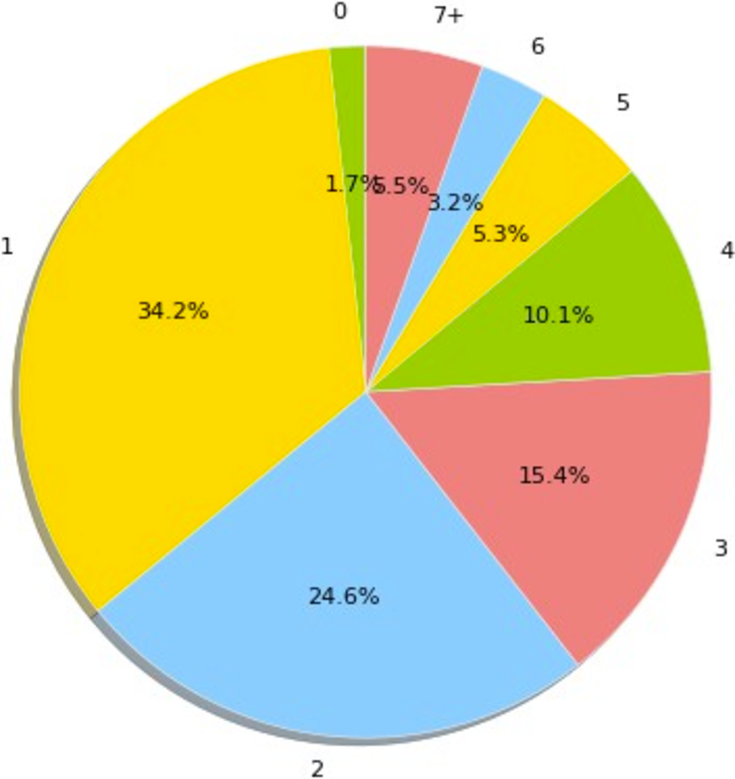
\includegraphics[width=0.5\linewidth]{resources/densities.pdf}
    \end{center}
    \caption{The distribution of densities (bounding boxes per image) in the DETECT dataset.  A density of 0 indicates that the image was taken containing no animals.  The maximum density of any image in the dataset is 23 but was capped at 7 (or more).  \copyright 2016 IEEE. Reprinted, with permission, from: J. Parham and C. Stewart, ``Detecting plains and Grevy’s zebras in the real world,'' in \textit{IEEE Winter Conf. Applicat. Comput. Vis. Workshops}, Lake Placid, NY, USA, Mar. 2016, pp. 1–9.}
    \label{fig:densities}
\end{figure}

The dataset is available\footnote{\url{https://cthulhu.dyn.wildme.io/public/datasets/detect.tar.gz} [18.0GB] (Accessed: Oct. 29, 2021).} as a Wildbook IA (WBIA)\footnote{\url{https://github.com/WildMeOrg/wildbook-ia} (Accessed: Oct. 29, 2021).} database for training and evaluation.  The data was split into subsets with 60\% for training, 20\% for validation, and 20\% for testing.  For all model training described in subsequent evaluations, the training and validation sets were combined, and the trained models were evaluated against only the test set.  The partitioning of the various sets, while random, was balanced to respect both the distribution of species and the number of annotations per image (see Figure~\ref{fig:densities} for a distribution).  The viewpoint was not considered for this balancing procedure because many of the images contain multiple photographed animals photographed from differing viewpoints.  A total of 501 images (with 1,343 ground-truth annotations) comprise the test set, which is for what the following results are reported.

The rest of this chapter will describe the core components of the detection pipeline in the order that they would be applied to an input image. The neural network models (except for the bounding box localizers) are trained using Lasagne~\cite{dieleman_lasagne_2015} and Theano~\cite{bergstra_theano:_2010,bastien_theano:_2012} on a single NVIDIA TITAN V GPU with 12GB of video memory\footnote{Much of this work was originally developed in 2016 and 2018.  Since then, most of the detection pipeline's components have been modernized and re-implemented with PyTorch~\cite{paszke_pytorch_2019} and are on PyPI under \texttt{wildbook-ia}}.  The localizer models are trained using 1) the original Caffe~\cite{jia_caffe:_2014} source code for Faster R-CNN\footnote{\url{https://github.com/rbgirshick/py-faster-rcnn} (Accessed: Oct. 29, 2021).}, 2) an original Python wrapper\footnote{\url{https://github.com/WildMeOrg/wbia-tpl-pydarknet} (Accessed: Oct. 29, 2021).} for the original YOLO V1 source\footnote{\url{https://github.com/pjreddie/darknet} (Accessed: Oct. 29, 2021).} by Redmon \textit{et al.}, and 3) a PyTorch~\cite{paszke_pytorch_2019} re-implementation \footnote{\url{https://github.com/WildMeOrg/wbia-deprecate-tpl-lightnet} (Accessed: Oct. 29, 2021).} by Ophoff \textit{et al.}~\cite{ophoff_lightnet_2018} of the original open-source implementation of YOLO v2.  The Python bindings\footnote{\url{https://github.com/WildMeOrg/wbia-tpl-pyrf} (Accessed: Oct. 29, 2021).} for the Hough Forests implementation by Gall \textit{et al.}~\cite{gall_hough_2011} are used for this evaluation.

\section{Whole-Image Classification (WIC)}\label{sec:wic}

The Whole-Image Classifier (WIC) is the first stage of the proposed detection pipeline.  Its primary goal is to make a ``relevancy check'' for all of the processing in the detection pipeline. Thus, for example, there would be no need to power up an advanced animal detection neural network and load its hefty weights into GPU memory for an image of a birthday party.\footnote{This is an actual situation that was encountered when the contents of an SD card was copied during a census.}  A benefit of using a first-pass image classifier is that -- due to advances in neural networks (see Chapter~\ref{chapter:related}) -- it can be trained with relatively little training data.  We can therefore expect this component to be very accurate and fast.  We analyze two use cases where the WIC is helpful for an automated animal detection pipeline: 1) checking for the existence of relevant species in an image for further processing, and 2) quickly processing large amounts of images to eliminate trivial negatives (e.g., filtering out false triggers made by camera traps).

\subsection{Species Existence Classifier}

One of the most common purposes of the whole-image classifier (WIC) is to quickly predict the existence of species of interest within an image.  Unlike the original ILSVRC classification challenge that offered only a dominant whole-image class with 1-class and 5-class testing modes, there is often a need to classify images containing multiple animal sightings for more than one species (of equal importance).  This distinction is important because some animal species (e.g., Gr\'evy's zebra and reticulated giraffes) have overlapping migratory ranges and are sometimes seen together in images.  Therefore, the WIC is designed to predict a multi-prediction, multi-target vector.  The vector's corresponding index is set to 1.0 if at least one animal of that species exists in the image and 0.0 otherwise.  Note that this network is not tasked to count the number of animals for a given species in the image.  Instead, it simply needs to produce a \textit{true} or \textit{false} flag for if the species exists.

The network takes as input a 192$\times$192-pixel image that is reduced to a 5$\times$5$\times$128 feature vector via convolutional and max-pooling layers.  The network then adds a 256-dimension dense layer, followed by a feature pooling layer, a dropout~\cite{hinton_improving_2012} layer ($p=0.5$), and another 256-dimension dense layer.  The final dense layer has six outputs, one for each species of interest, and uses a sigmoid activation function.  The design of the image classifier purposefully does not normalize the network's output with a softmax activation function, nor does it penalize for categorical cross-entropy loss.  As a result, the output is not a 1-hot vector and does not produce a discretized PDF that sums to 1.0.  For example, a valid network output could predict the existence of all (or none) of the target species in a given image.

\begin{figure}[!t]
    \begin{center}
        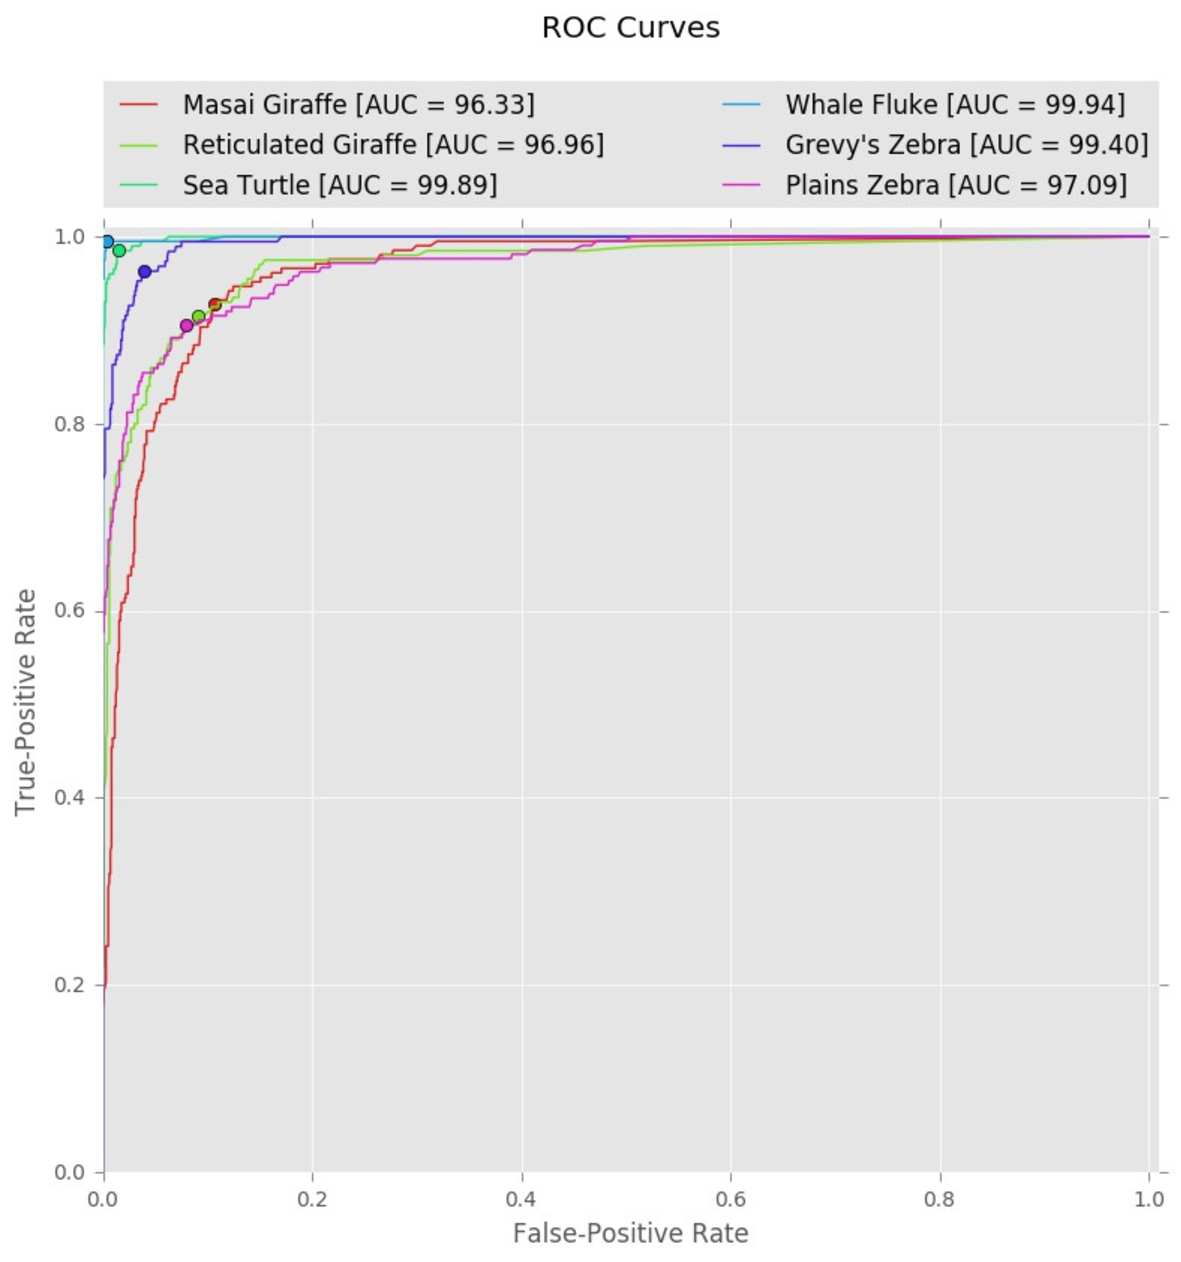
\includegraphics[width=0.9\linewidth]{resources/wic-roc.pdf}
    \end{center}
    \caption{The ROC performance curves for the Whole Image Classifier (WIC).  We can see that the WIC component of the detection pipeline performs extremely well on all species.  Some species are harder than others, notably giraffes and plains zebras; this error can be attributed to the similar appearance of the giraffe species, leading to confusion.  All species have an impressive AUC greater than 96\%, making it an accurate first-pass filter for the detection pipeline.  \copyright 2018 IEEE. Reprinted, with permission, from: J. Parham \textit{et al.}, ``An animal detection pipeline for identification,'' in \textit{IEEE Winter Conf. Applicat. Comput. Vis.}, Lake Tahoe, CA, USA, Mar. 2018, pp. 1–9.}
    \label{fig:performance-wic}
\end{figure}

For all of the neural network classifiers in the detection pipeline, extensive data augmentation is employed during training to help control over-fitting.  Data augmentation aims to provide the network with a slightly different training example for each epoch, sampled such that the mini-batches are also ordered randomly.  The augmentation is applied at runtime each time the training example is loaded into memory and not simply applied beforehand and cached to disk, saving disk space and increasing the amount of randomization during training.  The augmentation performs the following operations, each randomized for every training example:

\numsquishlist
\item exposure in the \texttt{Lab} color space on the luminance channel
\item slight hue shifts,
\item rotation, scaling, and Affine skewing,
\item horizontal flipping (generally no vertical flipping), and
\item blurring.
\numsquishend

The WIC model does an excellent job at correctly predicting species existence within an image, as shown in Figure~\ref{fig:performance-wic}.  The worst-performing species (Masai giraffe) achieves a ROC area-under-the-curve (AUC) of 96.3\%, and the best-performing species (whale fluke) has an almost-perfect 99.94\% AUC, missing only a handful.  The mean AUC across all species is an outstanding 98.3\%.  The operating points were selected as the closest values on the curve to the top-left corner (indicated by the colored dots on each curve), providing the optimal AUC and balancing the true-positive rate (TPR) against the false-positive rate (FPR).  With optimal points selected independently for each species, the image classifier can be used to predict an existence value for all six species simultaneously.  When we consider this use case, the classifier is correct 64.8\% of the time at predicting the exact X-hot vector for a given test image.  Nevertheless, the vast majority of the errors have a Hamming distance of 1, meaning the algorithm incorrectly predicts only one of the values in the vector.  Over 90\% of errors are between the two species of giraffe and zebra, predicting existence for both when only one is shown in the image.  Since the rest of the detection pipeline can distinguish between similar species, these errors are not a major concern because they should be caught by later, more focused (working with annotations, not images) components of the pipeline.

Using the WIC as a content filter is technically optional; we could choose to rely on the outputs of the second component, the localizer, to perform the initial content filtering. However, preliminary results by Beery \textit{et al.}~\cite{beery_recognition_2018} suggest that a localizer will slightly outperform a whole-image classifier at the filtering task on camera trap data but at the cost of much higher inference times. In addition, the WIC has significantly fewer parameters than the localization networks presented in the next section, which makes it much faster to run on large volumes of images.  For comparison, the WIC (run on batches of 1024 images) can return results in approximately 3-4 seconds using GPU acceleration.  In contrast, localization networks need to run smaller batches of around 128 (for memory reasons) and take upwards of 30 seconds (real-time) on the same GPU and images.  Therefore, the benefits of using a WIC with localization compared to using just a localizer can be profound when computational resources or runtime requirements for the application are limited.

\subsection{Filtering Camera Trap False-Alarm Triggers}

\begin{figure}[!t]
    \begin{center}
        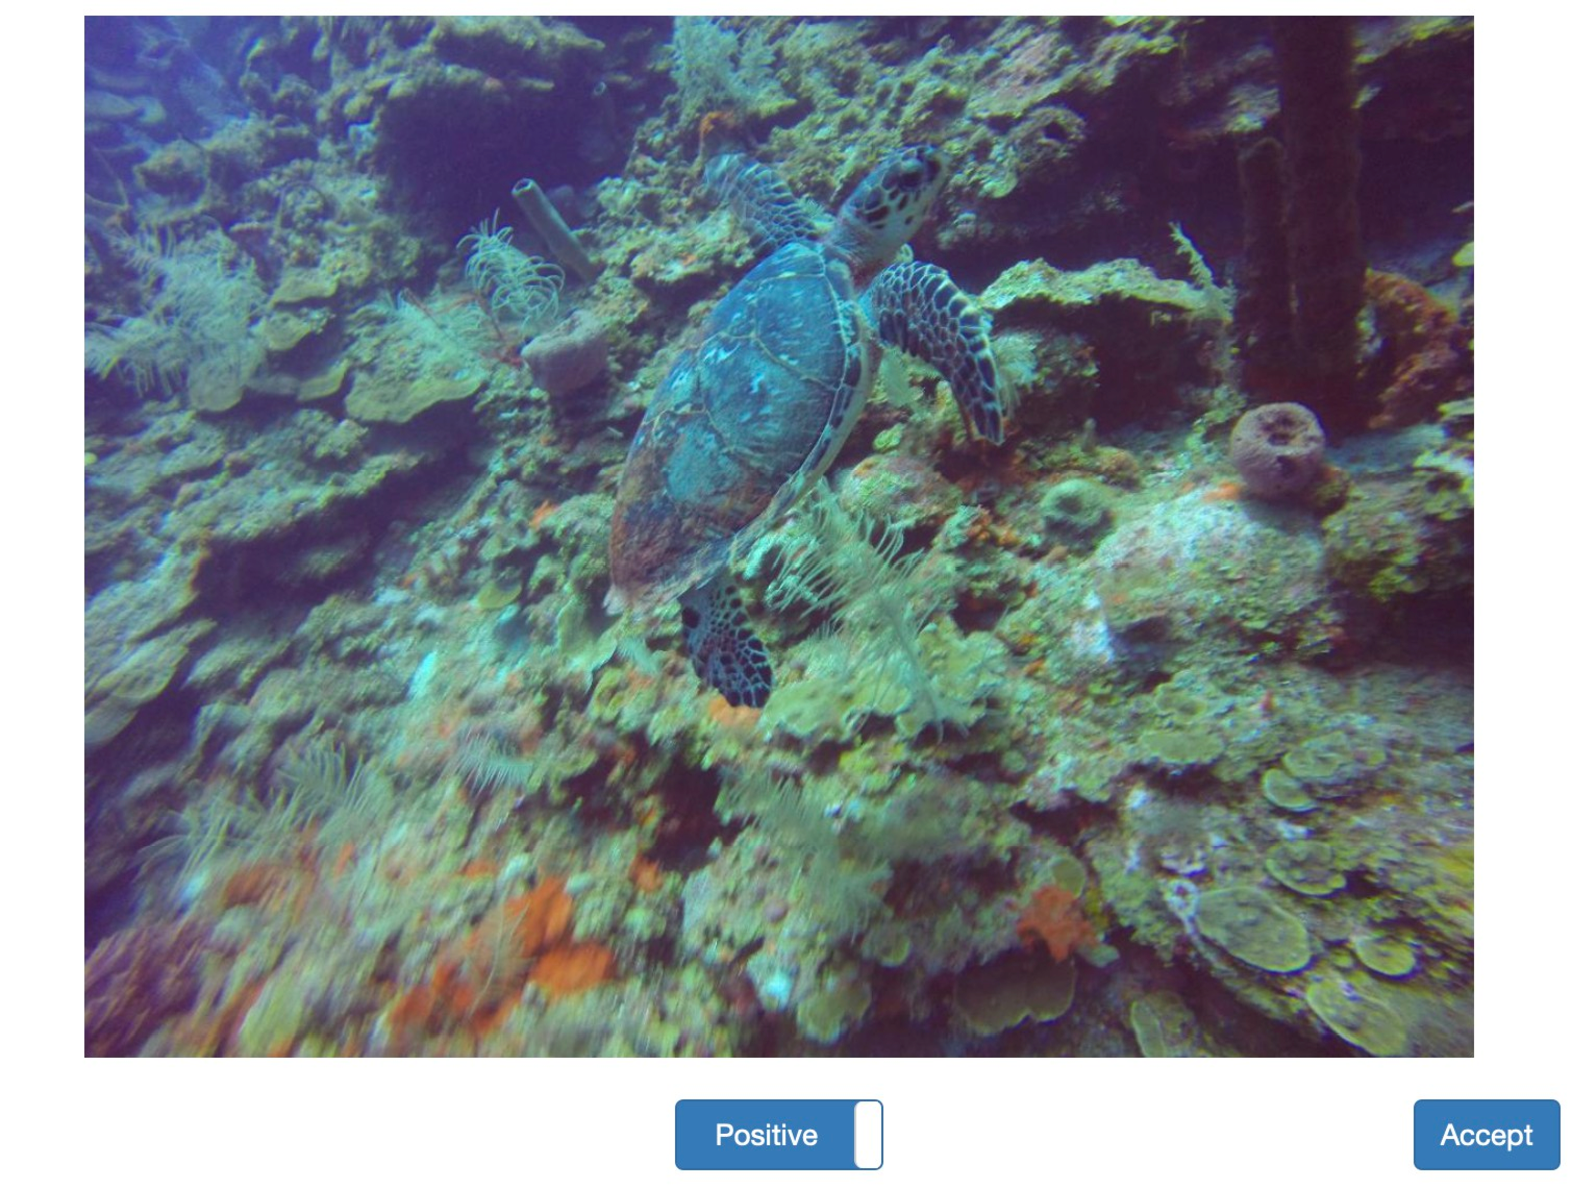
\includegraphics[width=0.8\linewidth]{resources/wic-interface.pdf}
    \end{center}
    \caption{The web interface for reviewing Whole Image Classifier ground-truth labels.  When using the WIC in binary mode, a simple flag on the entire image can be assigned for ``keep'' (positive) or ``discard'' (negative).  When run in the multi-prediction, multi-target mode, the localization web interface and subsequent annotations are used as the WIC's ground-truth training labels.}
    \label{fig:interface-wic}
\end{figure}

Another application for the whole-image classifier is to use it as a fast binary classifier to filter out irrelevant images.  One example of where this function is valuable is very quickly processing raw images taken by a camera trap or aerial survey.  Images collected by a motion-triggered camera trap are expected to have a high ratio of false positives because the trigger is not context-aware (i.e., images taken that do not contain any sightings of desired species).  To set the scale of this problem: the WIC classifier could, for example, be used to search through 500,000 camera trap images to find less than 1,000 that had sightings of aquatic jaguar (\textit{Panthera onca}).  The sheer size of the problem is an issue for running slower localization algorithms on this amount of data and generating sufficient training data to train the WIC (or localizer) on novel camera trap collections with minuscule true-positive rates.

\begin{figure}[!t]
    \begin{center}
        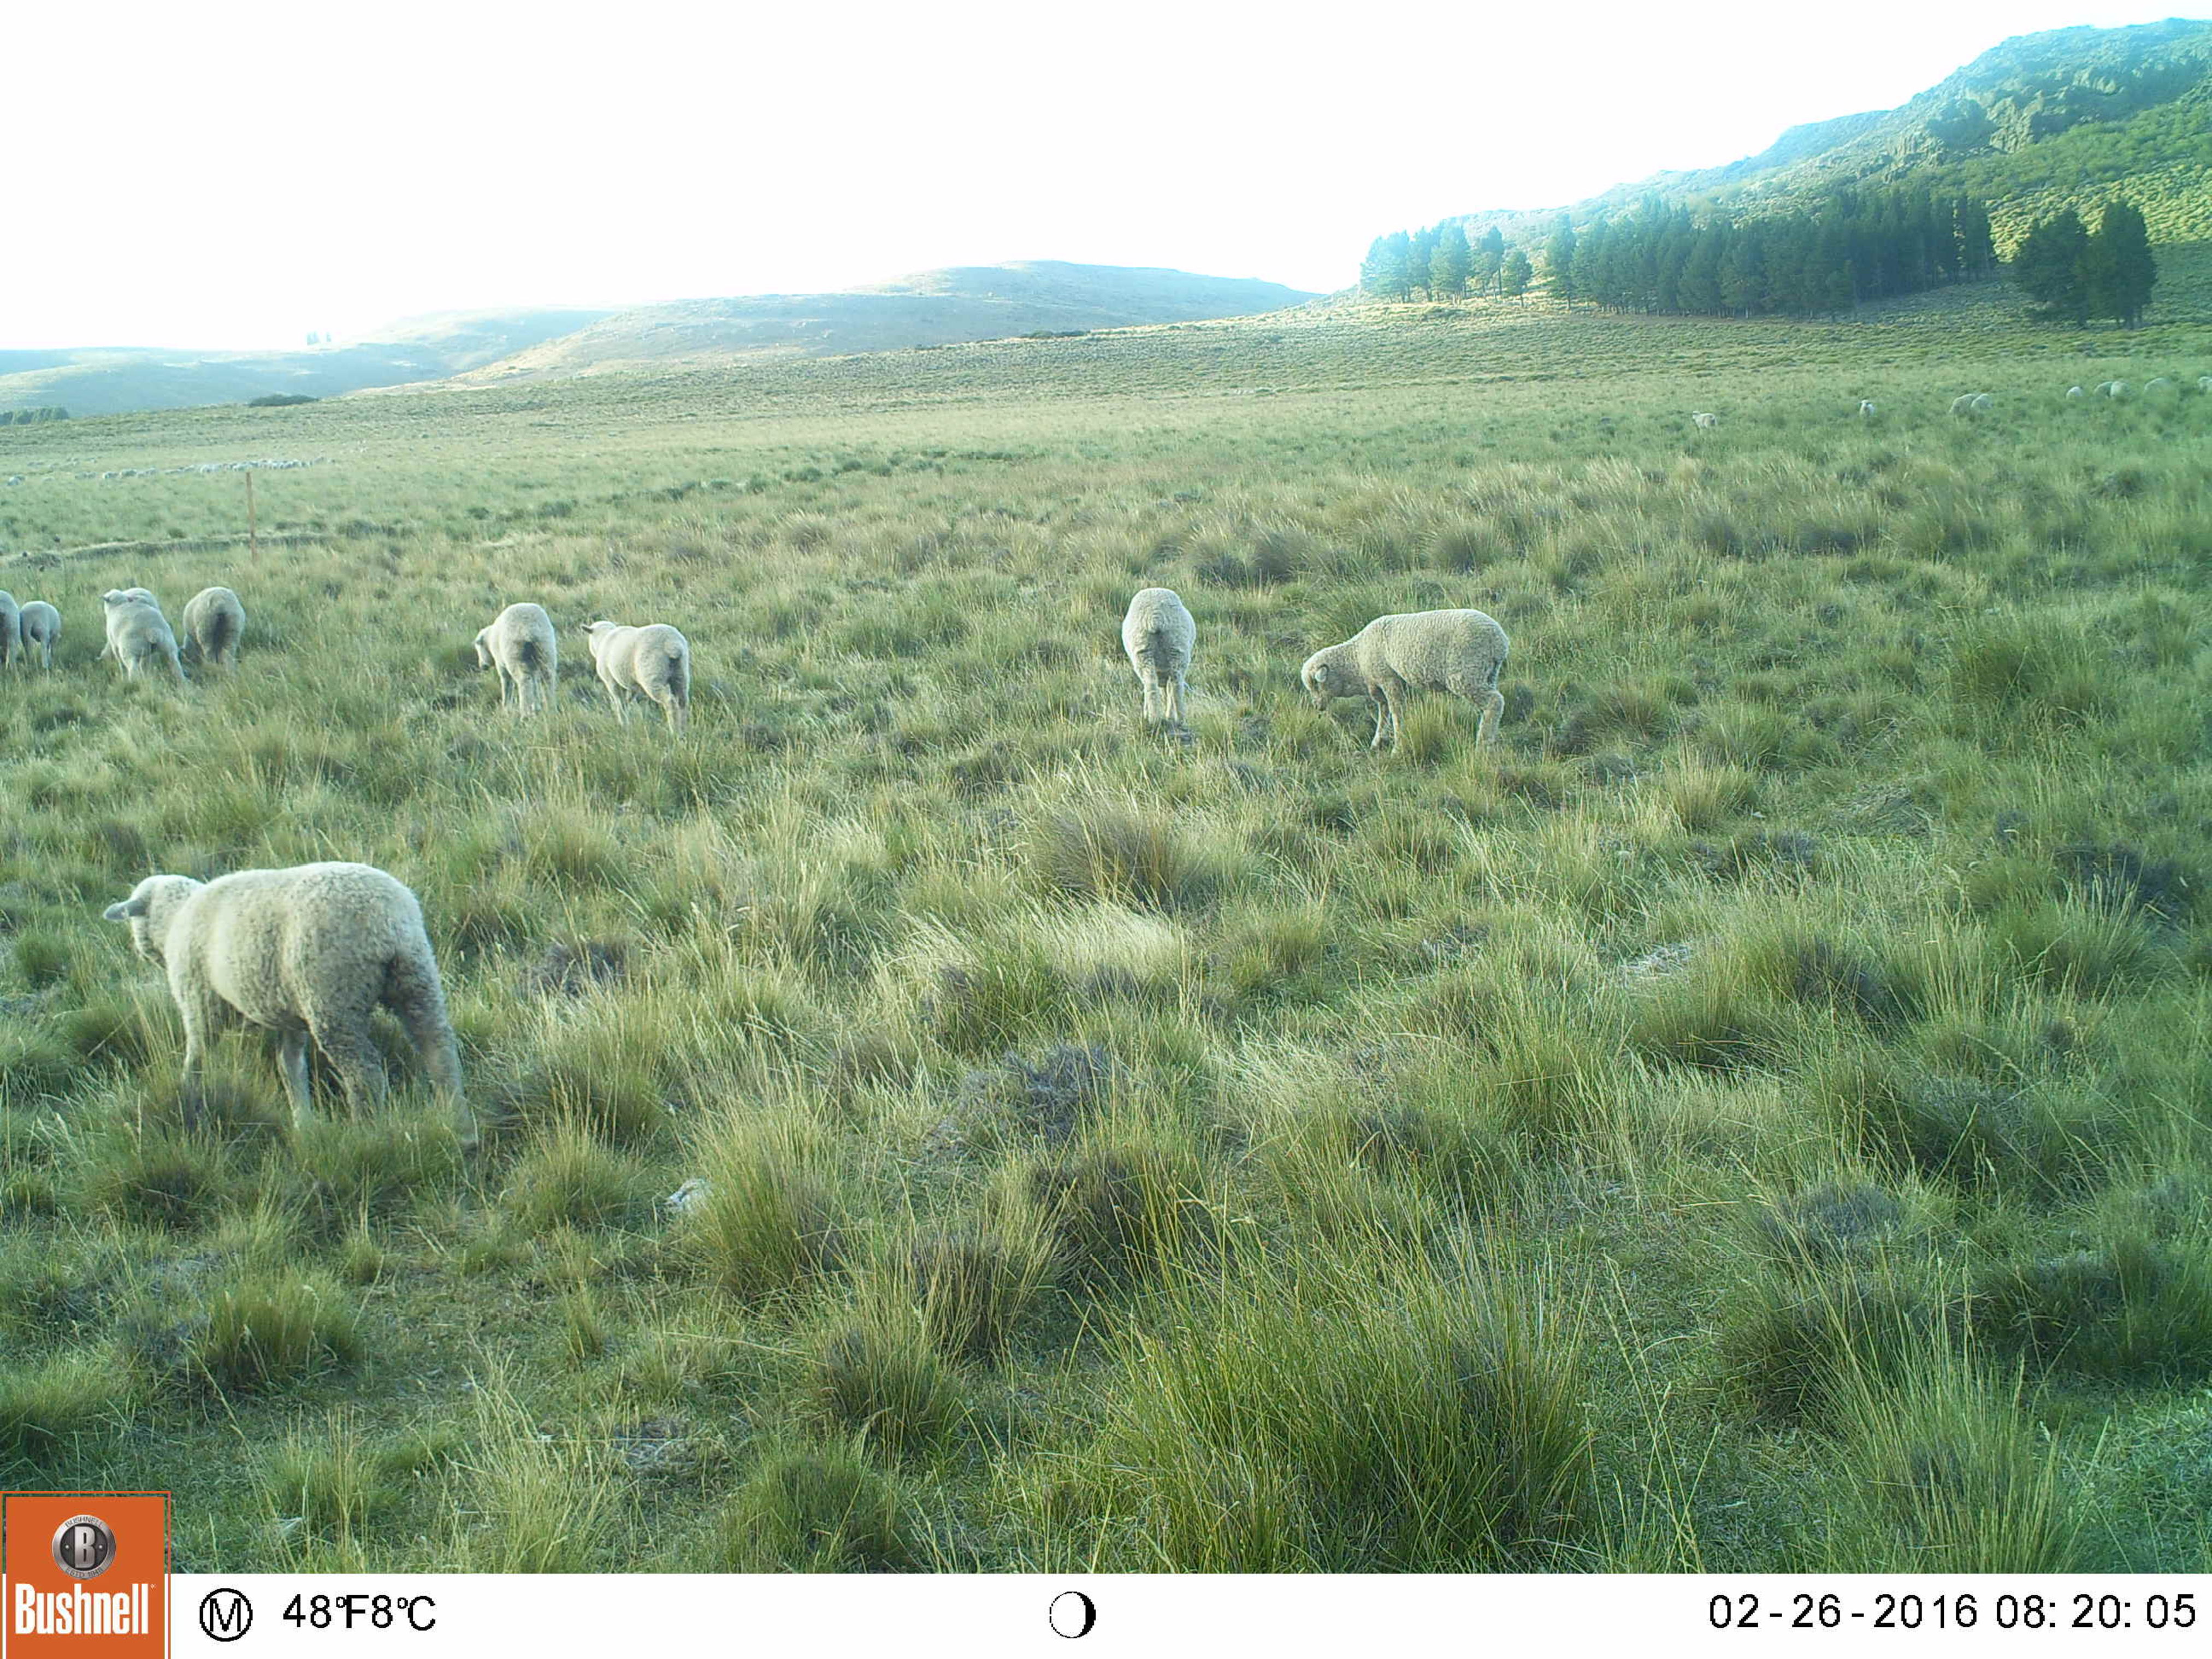
\includegraphics[width=0.47\linewidth]{resources/cameratrap-dataset1-positive.pdf}
        \hspace{1mm}
        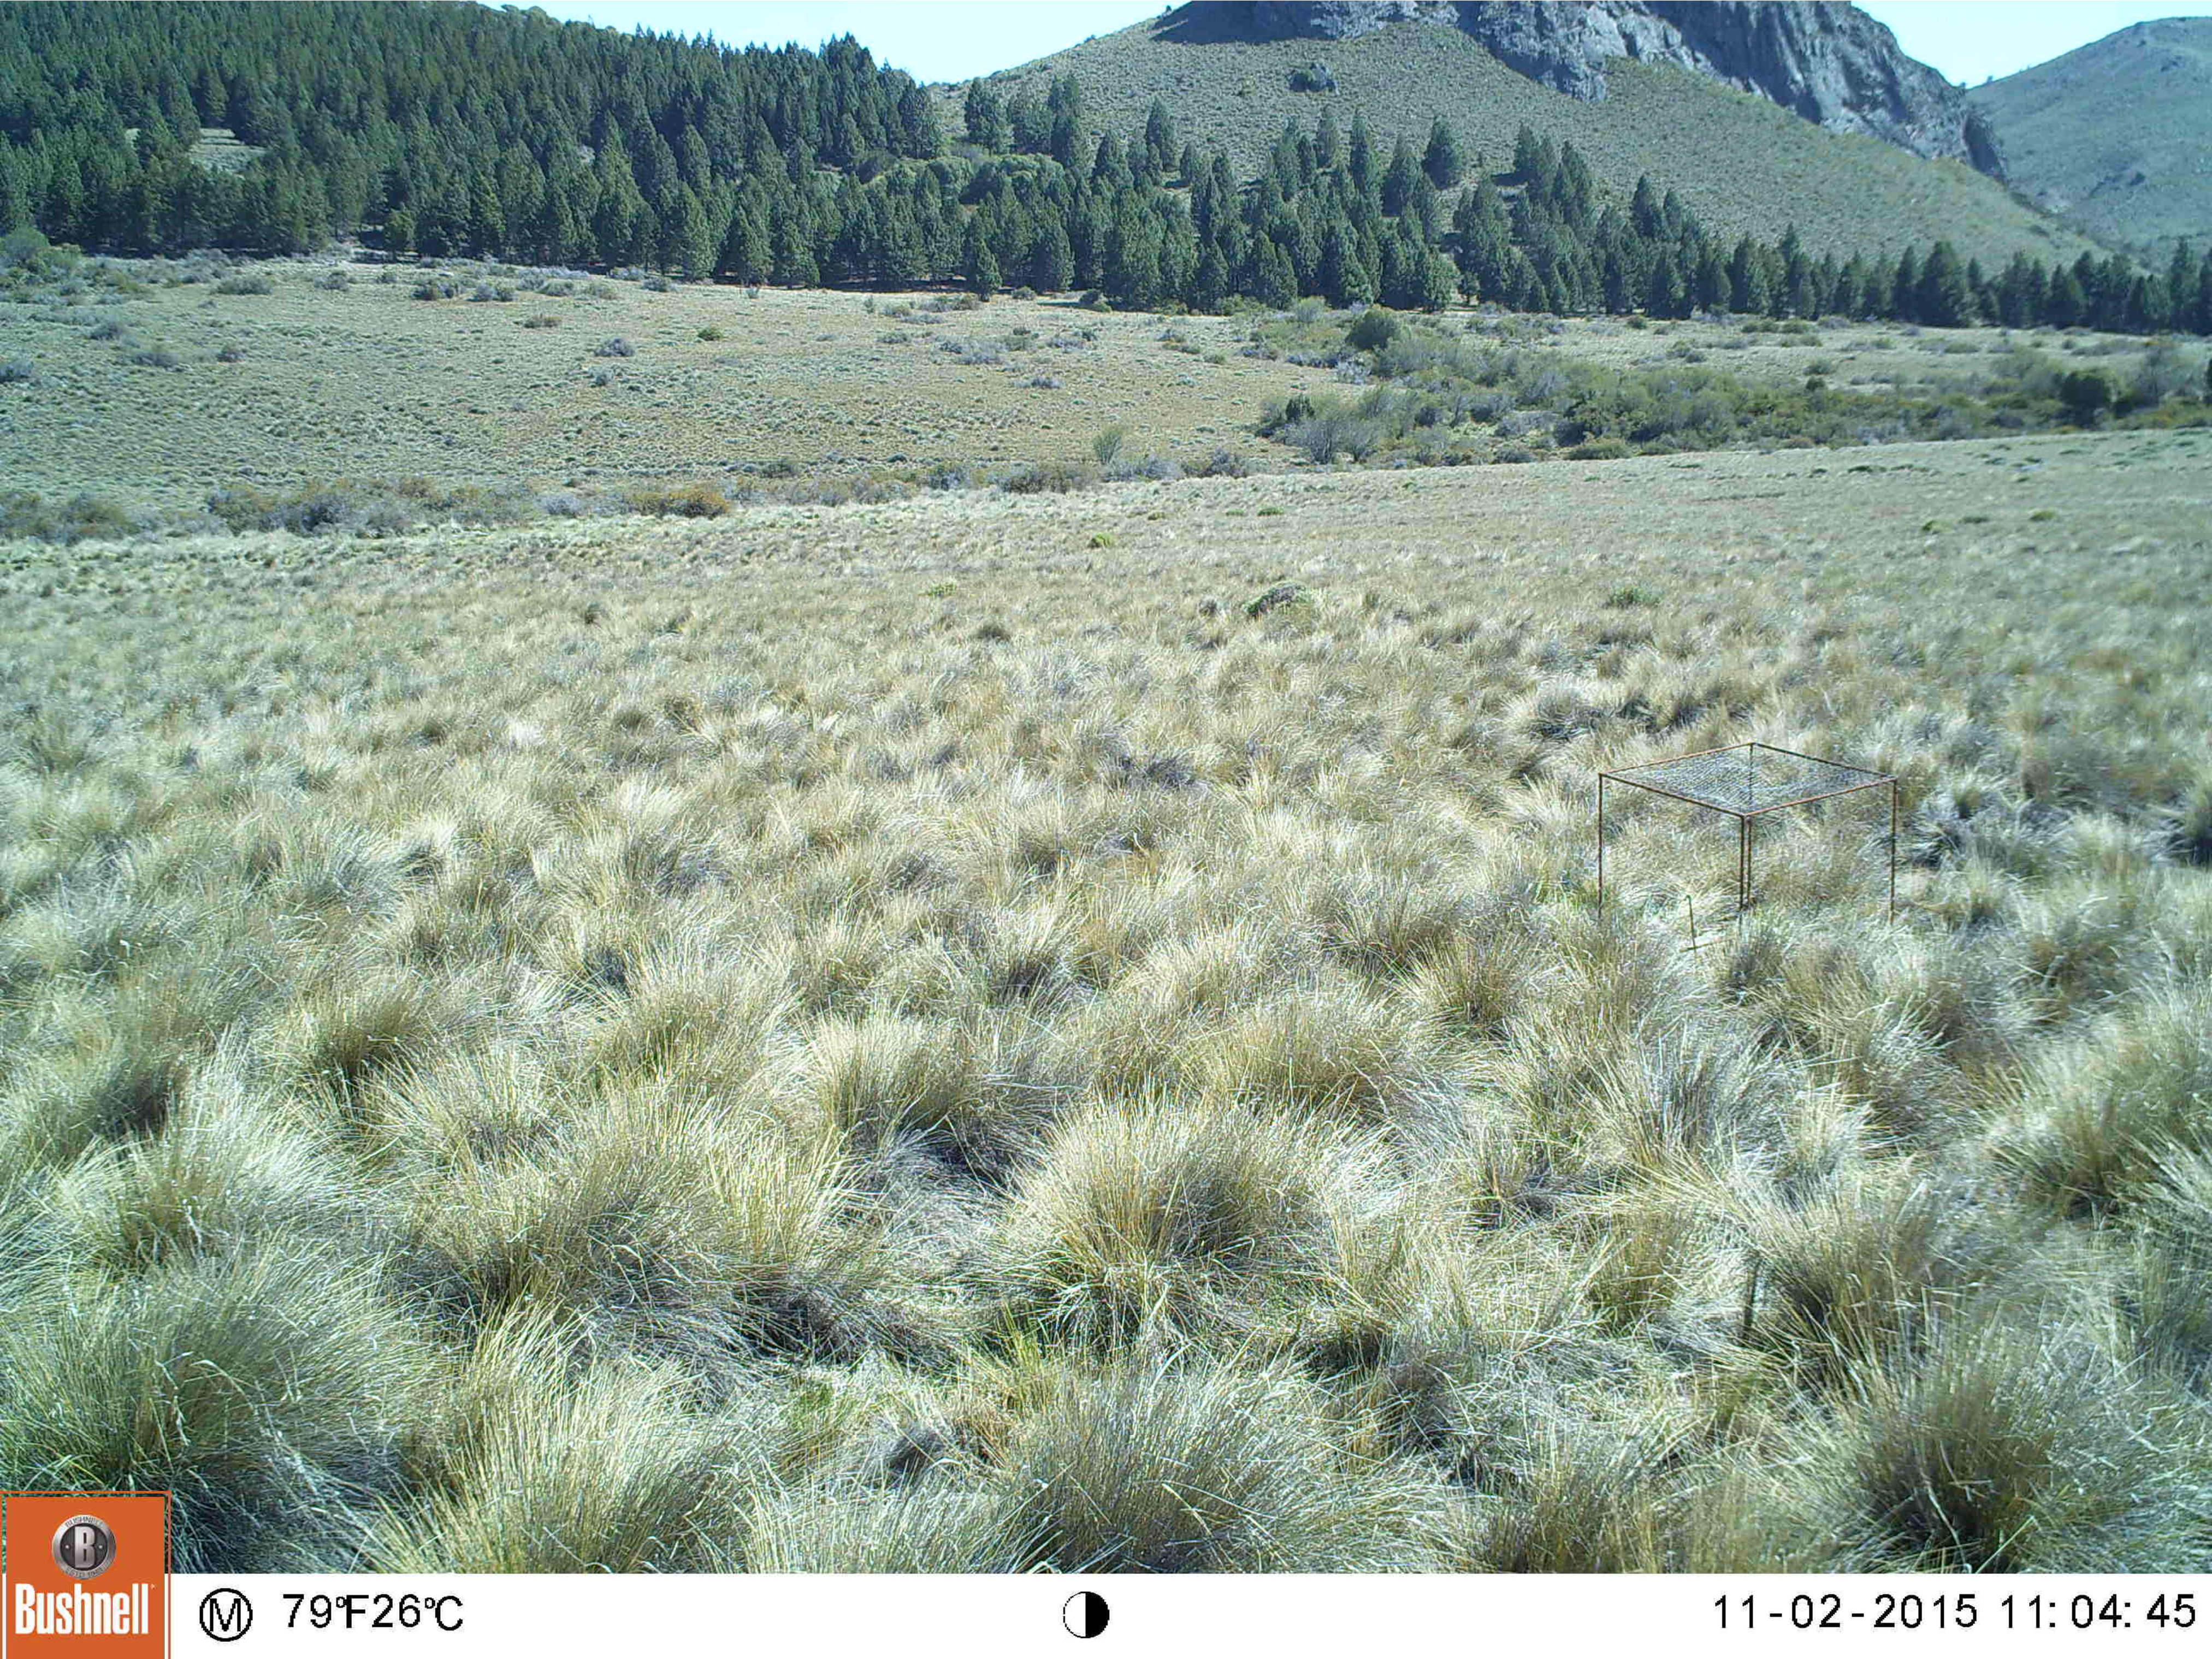
\includegraphics[width=0.47\linewidth]{resources/cameratrap-dataset1-negative.pdf}
    \end{center}
    \caption{Example camera trap images of true-positive (left, animals detected) and false-positive (right, nothing of interest) triggers, taken from two camera-trap datasets.}
    \label{fig:example-wic-cameratrap}
\end{figure}

Fundamentally, we can re-formulate the WIC as a simple binary classifier (2 classes with standard cross-entropy loss) that predicts either ``keep'' or ``discard'' for a given image.  The benefit of a binary design is that it can be very flexible, allowing a camera trap researcher to decide the usefulness of an image in whatever way is needed.  A web interface was designed to give a randomized example to a reviewer for annotation, as shown in Figure~\ref{fig:interface-wic}.  The benefit of this tool is that it allows a researcher to quickly create ground-truth for training the WIC component that is tuned for a unique camera trap location and survey time, often to create a one-time-use ML model.  One of the apparent benefits of using the WIC as a filter for camera trap images is that it does not require extensive (and relatively labor-intensive) bounding-box training data.  If available, the network can use bounding boxes to specify existence ground-truth (essentially a ``yes'' or ``no'' value for keeping an image), but this is not a requirement.  As such, gathering a large amount of training data for the WIC is manageable and efficient because it can be trivially distributed to multiple human annotators.

\begin{figure}[!t]
    \begin{center}
        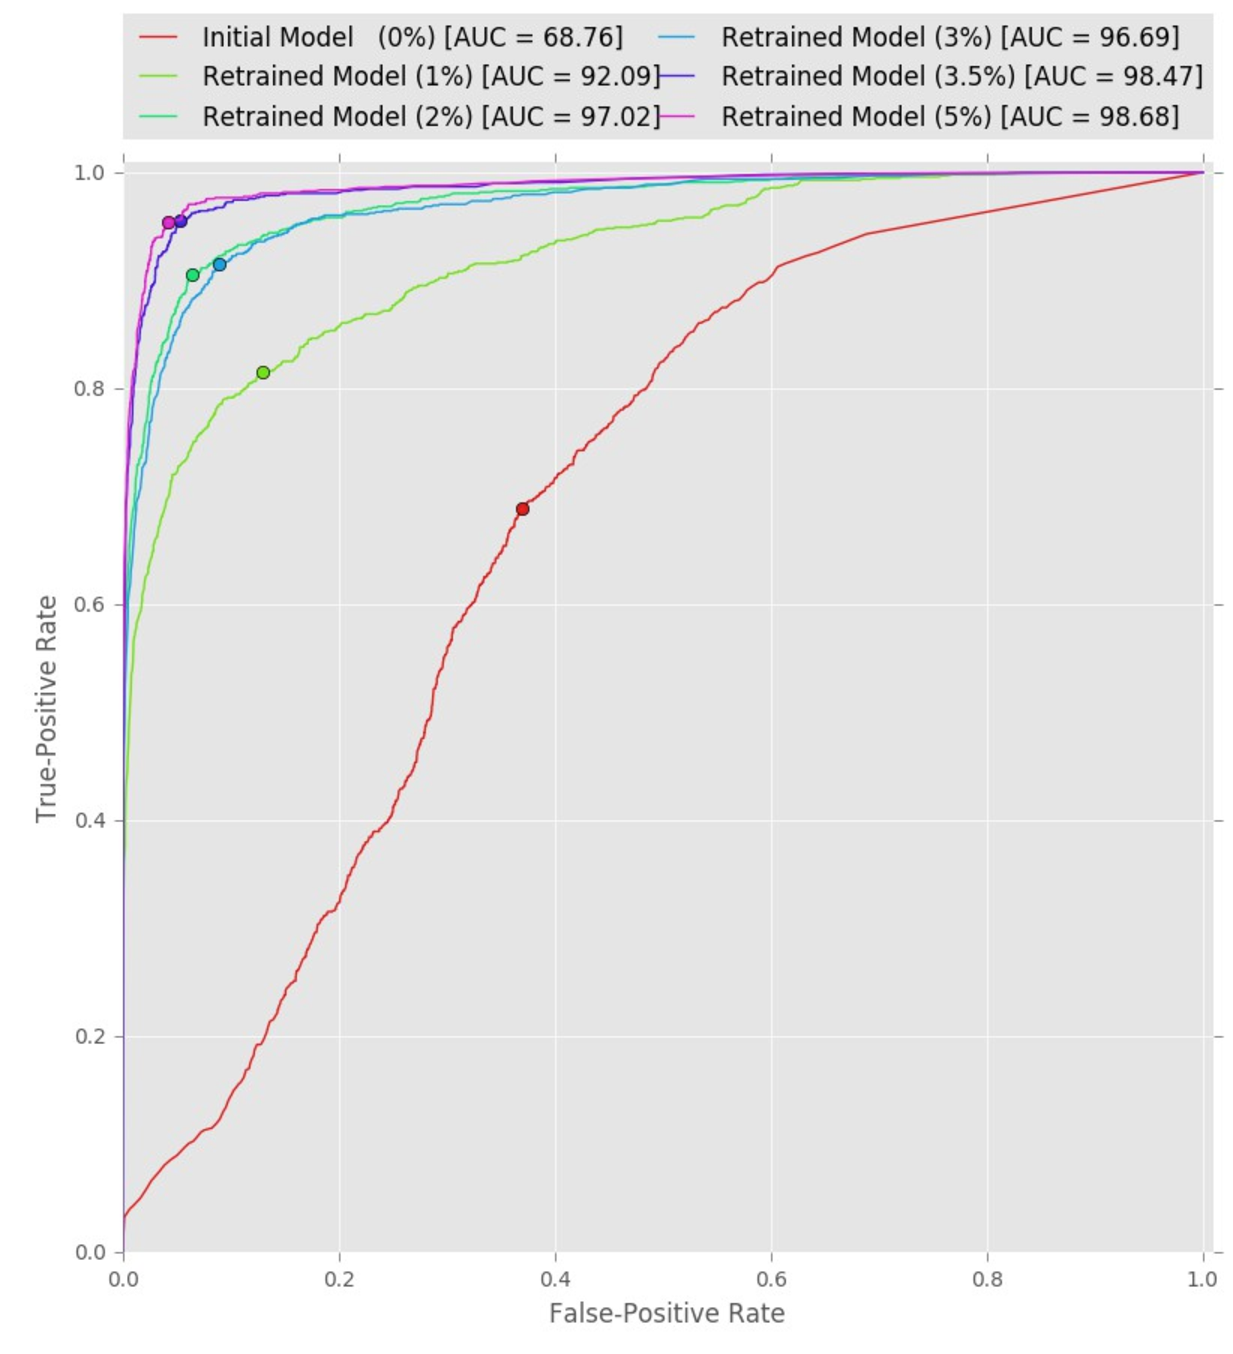
\includegraphics[width=0.7\linewidth]{resources/classifier-roc-megan1.pdf}
    \end{center}
    \caption{The ROC performance curves for the Whole Image Classifier on camera trap photographs.  The best model with 5\% of the data annotated achieves a classification accuracy of 96.5\%.}
    \label{fig:performance-wic-cameratrap}
\end{figure}

The results of the WIC are presented here on a proprietary dataset captured by Dr.\ Megan McSherry at Princeton University using motion-based camera traps in Kenya.  While state-of-the-art results on this task are not reported here, a benchmark of the WIC classifier is presented for future baseline comparisons.  We refer the reader to the work of Beery \textit{et al.}~\cite{beery_recognition_2018} for a more advanced framework on how to detect animal movement in camera traps.  The dataset was captured with camera traps placed in specific areas to photograph domesticated grazing of herding animals by local tribes.  Figure~\ref{fig:example-wic-cameratrap} gives an example of a positive and negative image -- we see that (left) shows sightings of sheep and (right) is an empty field with nothing of interest (a false trigger).  An initial model was trained using a baseline ground-truth split between a few hundred positive and negative images provided by the researchers (referred to as the 0\% split).  New WIC models were then trained using hand-annotated ground-truth data, in approximate intervals of 1\% of the total size of the dataset, up to 5\%.  Figure~\ref{fig:performance-wic-cameratrap} shows the performance of each WIC model as more ground-truth examples were provided.  Even with only 1\% of the entire dataset annotated, the WIC model can achieve an impressive Area Under the Curve (AUC) of 92.1\%.  Annotating a total of 5\% of the data results in a final classifier that achieves 98.7\% AUC on held-out validation data.  However, we can see that the performance increase with more ground-truthed training data quickly diminishes; effectively, the dataset could have only been annotated to 3.5\% (98.5\%) for approximately the same performance level as 5\% (98.7\%).  These results show that the WIC can be a highly effective and accurate tool for filtering camera trap imagery while putting light expectations on data annotation.  The evaluation focuses on small amounts of training data.  It shows that annotating even a 1\% random data sampling can perform as a weak classifier to eliminate many false-alarm images (92.1\% AUC).

After the WIC is applied to the raw images and filtered appropriately, the next step of the detection pipeline is to localize all of the relevant animals in the images.  This step is crucial because images may contain multiple animals, or the animal could be small relative to the size of the image. Therefore, some process is needed to convert images into annotations of distinct animals for the identification procedure.

\section{Annotation Bounding Box Localization}

The second component of the detection pipeline is tasked with generating bounding boxes and species labels for the relevant animals in an image.  Localization is vital from an identification perspective because it allows for the separation of distinct animals, gives a consistent and comparable scale of the different sightings, and supplies a method (cropping) to remove large amounts of distracting background information.  Furthermore, the preciseness of the bounding boxes (i.e., how well they fit snugly around an animal) can play a critical role in the overall accuracy of the identification pipeline, something that will be examined in-depth in later chapters.  After all, annotations are the primary lens through which ID sees the world, and the localizer should be very careful not to produce confusing or poorly-formed bounding boxes.  This filtering role also means that the quality of the localization component plays a crucial role in the overall quality of a photographic census. Hence, it is a significant focus of evaluation in this chapter.

\begin{figure}[!t]
    \begin{center}
        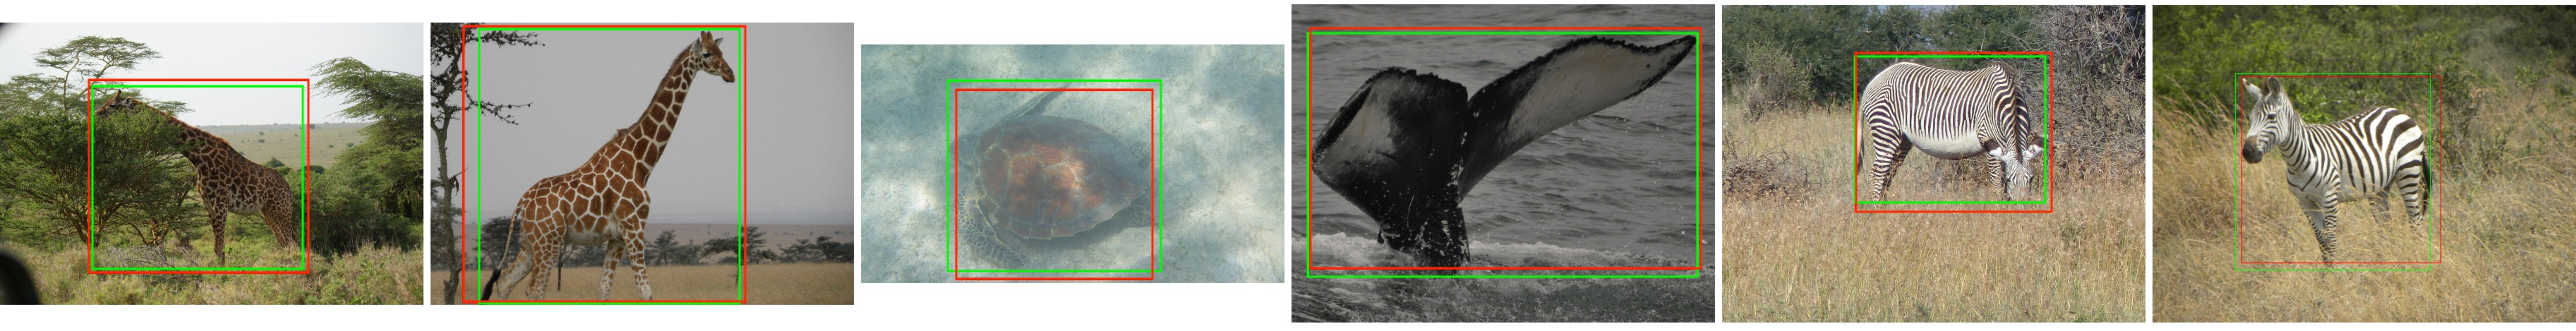
\includegraphics[width=1.0\linewidth]{resources/localizations.pdf}
    \end{center}
    \caption{Example annotation localization predictions on single-sighting exemplar images for each of the six species of interest in the WILD dataset.  The green boxes designate ground-truth bounding box coordinates, and the red boxes represent the localization bounding box predictions.  Since annotation classification is also performed, these bounding boxes are treated more like salient object detections.  \copyright 2018 IEEE. Reprinted, with permission, from: J. Parham \textit{et al.}, ``An animal detection pipeline for identification,'' in \textit{IEEE Winter Conf. Applicat. Comput. Vis.}, Lake Tahoe, CA, USA, Mar. 2018, pp. 1–9.}
    \label{fig:localizations}
\end{figure}

Two fundamentally different detection techniques for the localization component are compared: a pre-neural network approach and (two) neural network approaches.  As perplexing as it may seem in the era of deep learning to use anything but a neural network, random forest detectors are easy to train because they have fewer hyper-parameters, built-in regularization, and require much less data to train.  Furthermore, they do not rely on heavy GPU-accelerated computation for training, making them an ideal candidate for bootstrapping when few training images are available.  The Hough Forests~\cite{gall_class-specific_2009} variant of random forests, in particular, is resilient to partial and occluded objects due to its voting scheme~\cite{winn_layout_2006}.  As such, a random forest-based detector and two CNN-based detectors (Faster R-CNN~\cite{ren_faster_2015} and YOLO v2~\cite{redmon_yolo9000:_2016}) are evaluated on the WILD Dataset.

Before we begin, we need to review exactly how a bounding box is defined.  A bounding box $i$ for a given image $I$ is parameterized by the following equation:

\begin{align}
    \begin{split}
        \text{bbox}_{i}(Image, x, y, w, h, \theta) &= \text{rotate}(I \lbrack y: y + h \rbrack \lbrack x: x + w \rbrack \lbrack:\rbrack, \theta)
    \end{split}
\end{align}

\noindent where cropping is applied before rotating around the center of the bounding box.  While the localization algorithms presented in this section do not apply any rotation directly (and only predict axis-aligned bounding boxes with species labels), a separate orientation component can rotate and fix the boxes if needed.  The orientation task is a separate module because it allows the localizer to be replaced without requiring the new algorithm to support rotation (a relatively rare need).  It is also worth noting quickly that not all animals in an image are worth localizing.  For example, small birds or very distant animal herds are ignored in this evaluation because they are categorically not the focus of censusing events, especially since it can be exceedingly tedious to annotate ground-truth thoroughly. Thus, while ground-truth completeness in bounding boxes is crucial, there is a point where it is simply not realistic to perfectly annotate (or automatically find) every single animal in an image.
Examples of easy object localizations for each of the six species in the WILD dataset can be viewed in Figure~\ref{fig:localizations}.

\subsection{Hough Random Forests (RF)}

Hough Forests are an ensemble of random binary trees.  Each tree attempts to optimize the performance of classification and regression by performing a series of binary pixel tests; the authors of~\cite{gall_class-specific_2009, leibe_robust_2008} demonstrate that training a random forest tree in this combined fashion benefits both generalization and accuracy.  The first pre-processing step of training extracts a collection of small image patches (32$\times$32 pixels) from the ground-truth to compose a large set (60,000) of positive and negative training patches.  Importantly, each positive patch records its relative offset to the center of its corresponding object in the ground-truth.

During training, each tree is given the same set of patches.  The implementation used in this evaluation has an ensemble -- hence, a ``forest'' -- of 10 trees.  Each tree generates tests that split the patch dataset at each non-leaf node, which performs a random binary pixel test on each image patch $P$.  The test, as formulated in~\cite{gall_hough_2011}, is

\begin{align}
    \begin{split}
        test_{\alpha,p,q,r,s,\tau}(P) &=
        \begin{cases}
            0, & \text{if } P^\alpha(p,q) < P^\alpha(r,s) + \tau \\
            1, & \text{otherwise}
        \end{cases}
    \end{split}
\end{align}

\noindent
where $\alpha$ is the channel of the image patch, $(p,q)$ is a random location in the patch, $(r,s)$ is a different random location in the patch, and $\tau$ is a threshold offset.  Every node is allowed to pick a unique randomized test, randomly seeded to promote diversity.  Every node samples randomly over the parameters $\alpha,p,q,r,s,\tau$ to find the best binary test that minimizes either the positive-negative classification error or the positive-patch regression error.  The node will minimize (with $p=0.5$) either the binary cross-entropy classification error or the regression offset sum-squared difference error (negative patches are ignored since, by definition, they have no center offset to an object center).  Each tree is constructed recursively to a depth of 16 layers during training or creates a leaf when a node has fewer than 20 patches.

\begin{figure}[!t]
    \begin{center}
        \begin{tabular}{ccc}
            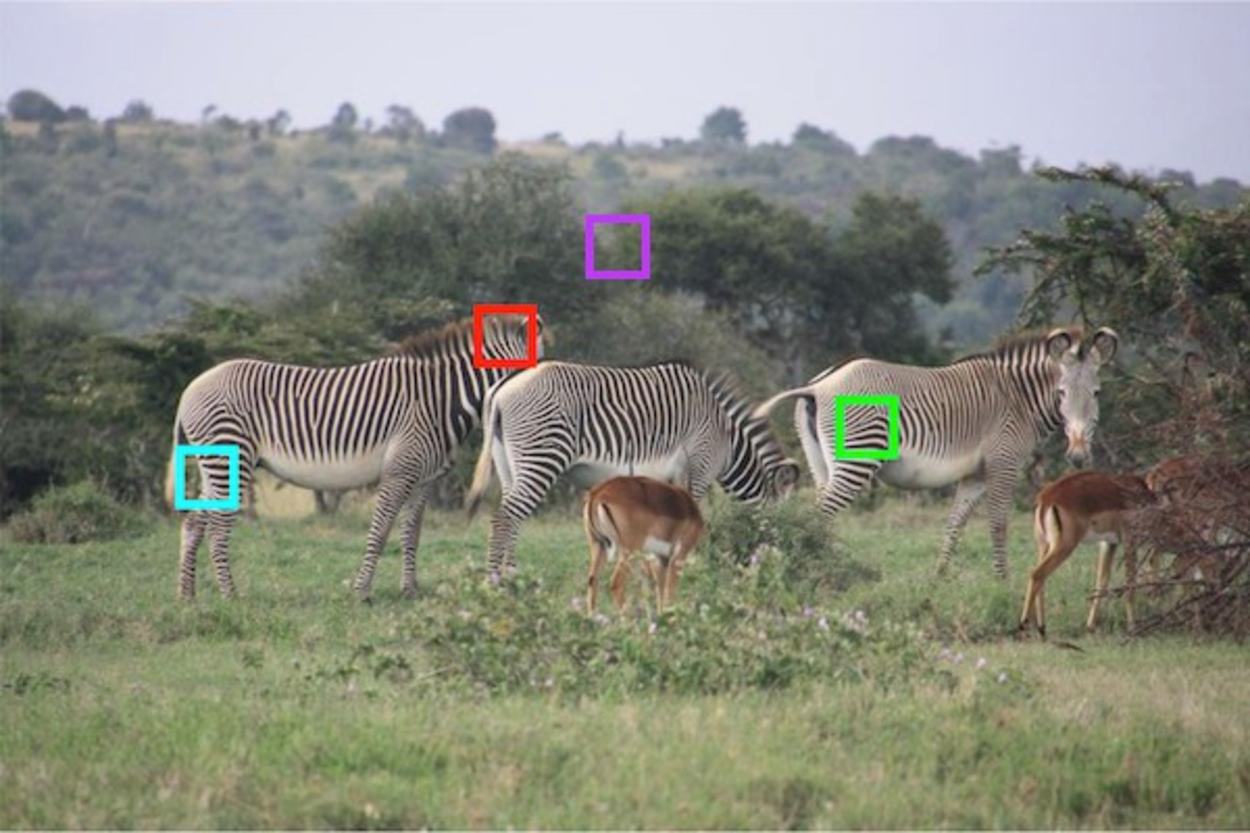
\includegraphics[width=0.3\linewidth]{resources/rf1.pdf} &
            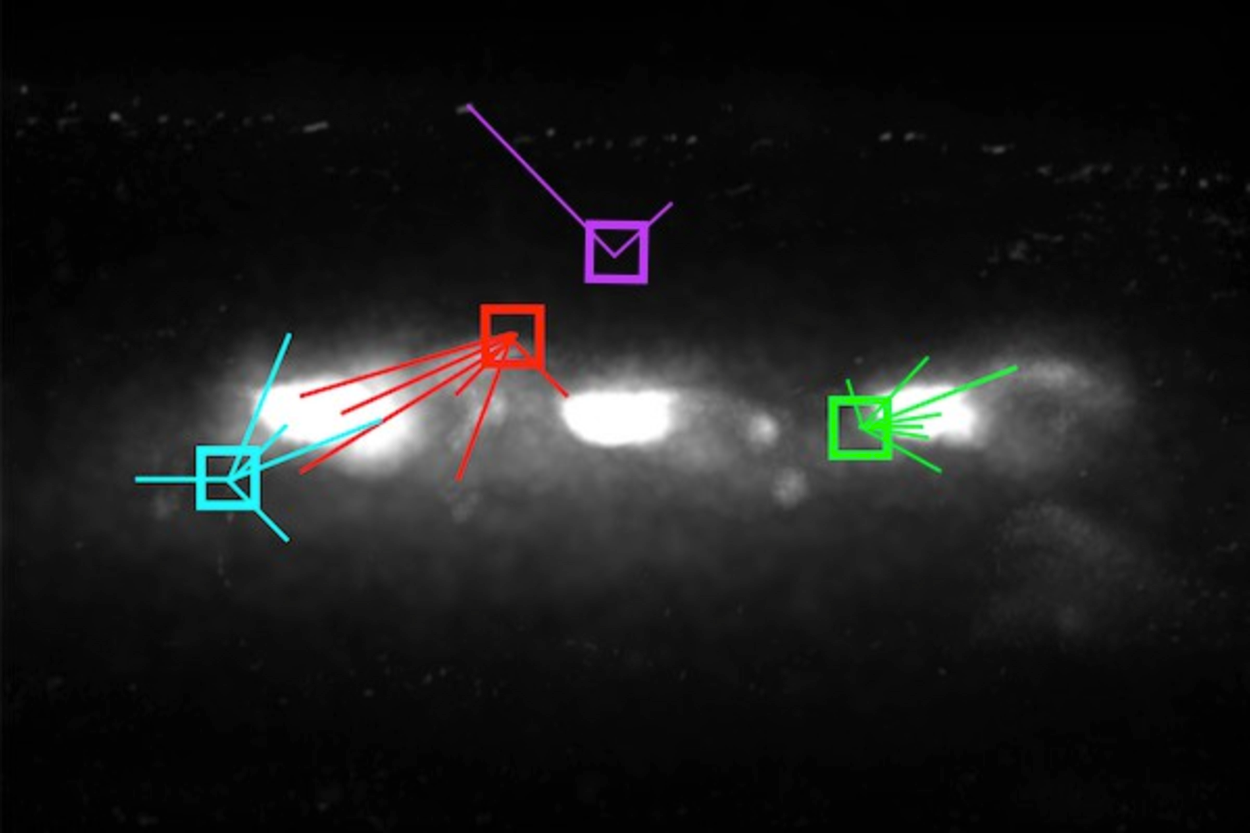
\includegraphics[width=0.3\linewidth]{resources/rf2.pdf} &
            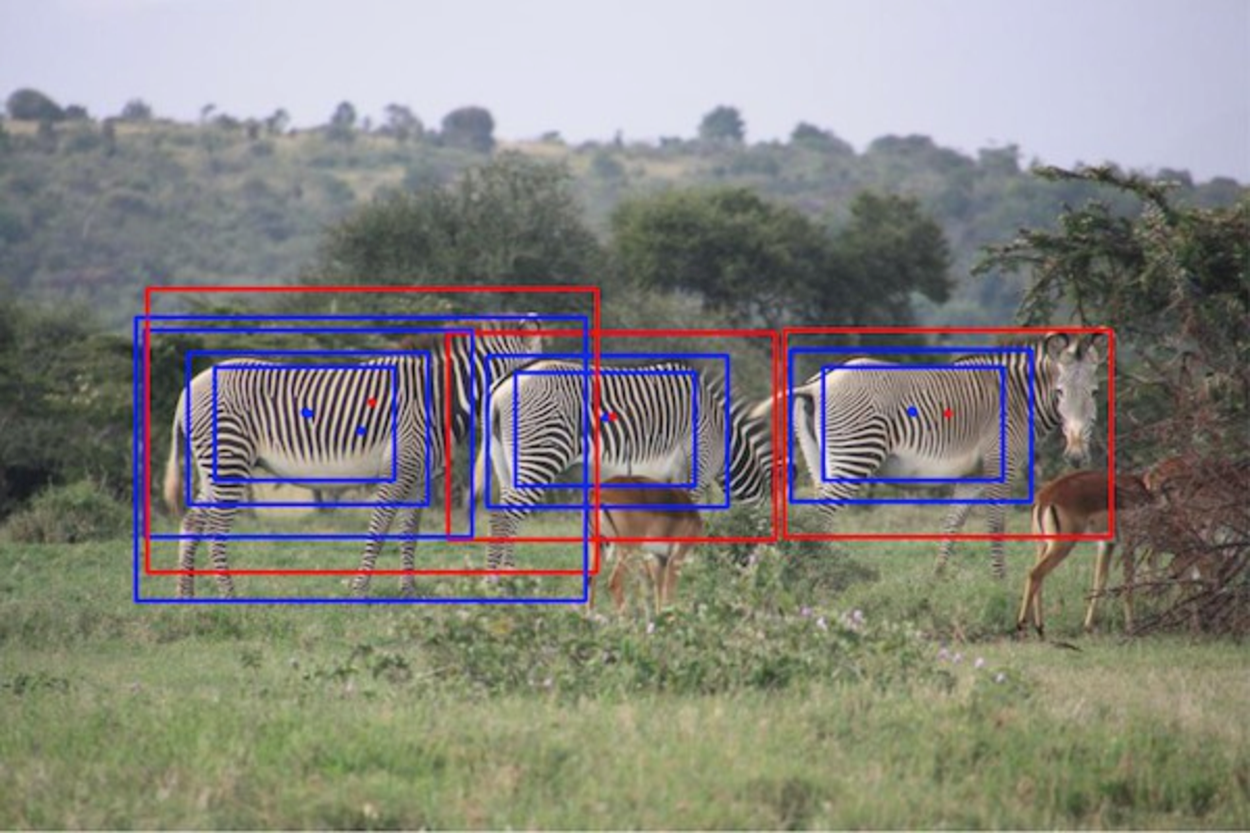
\includegraphics[width=0.3\linewidth]{resources/rf3.pdf}   \\
            (a) Source Image                                         &
            (b) Hough Image                                          &
            (c) Final Detections
        \end{tabular}
    \end{center}
    \caption{Hough Forests test patches are extracted densely over a test image (a) and are classified using an ensemble of random binary trees into a collection of leaves.  Each leaf has a set of positive and negative patches given to it during training, which are used to make weighted probabilistic Hough votes into an aggregate Hough image (b).  The high-probability object center peaks (white) are used to generate bounding box proposals (c, blue).  The proposals are filtered with non-maximum suppression to create the final detections (c, red).  Compare the votes of the red and purple test patches in (a, b); the purple votes are sporadic and do not accumulate, whereas the red votes contribute to an object center.  The blurring on peaks is due to voting confusion.  \copyright 2016 IEEE. Reprinted, with permission, from: J. Parham and C. Stewart, ``Detecting plains and Grevy’s zebras in the real world,'' in \textit{IEEE Winter Conf. Applicat. Comput. Vis. Workshops}, Lake Placid, NY, USA, Mar. 2016, pp. 1–9.}
    \label{fig:randomforest}
\end{figure}

During test time, each leaf node holds a collection of positive and negative patches.  A leaf's positive class probability is computed as the percentage of positive patches out of all patches it received by the end of training.  Each positive patch in a leaf makes a weighted probabilistic vote for the object's center in the test image based on where that patch originated in its respective ground-truth image.  As shown in Figure~\ref{fig:randomforest}, these Hough-transform votes (a) are computed densely across the entire test image and aggregated over multiple scales to generate a combined Hough image (b).  The bright white spots in the Hough image indicate the probable locations of object centers.  Thresholded peaks are selected as candidate center proposals, object bounding boxes are derived from the locations of patches that voted for the particular peaks (c, blue), and non-maximum suppression is applied to produce the final detection regions (c, red).

The Hough Forests detector has some distinct advantages: 1) it is easy to parallelize across multiple CPU cores for efficient training and inference processing, and 2) the voting scheme will aggregate probabilities originating from \textit{any} location on an animal.  For example, if only the face and neck of a zebra are visible in an image, the face and neck tree leaves will still make probabilistic votes for where it thinks the center of a zebra should be, even if that location is off the edge of the image or is occluded.  This voting scheme makes Hough Forests more resilient to occlusions and makes it an attractive solution to the challenges present in the WILD dataset.  However, the image patches are too small to learn precise localization information (i.e., a zebra neck patch can look very similar to a zebra hip), which results in a distinct blooming effect of voting confusion surrounding an object's center in the Hough image.  Moreover, the implementation of Hough Forests used here is trained as a binary classifier (one-vs-all) and, therefore, cannot natively represent multiple classes within the same tree.  This limitation poses a problem with representing multiple poses of the same species, as some views have conflicting spatial representations for an object's center.  This conflict confuses training and detection, which hurts accuracy.

The evaluated version of Hough Forests improves on the efficiency and accuracy reported in~\cite{gall_hough_2011}.  The implementation adds OpenMP\cite{openmp08} multi-CPU parallelization, adds new image channels, supports multiple resolutions, drastically increases the number of binary tests performed at each node during training, and makes more intelligent bounding box regression decisions with the coordinates of voting patches.  The details explained in this section are meant to augment the algorithmic summary in previous work~\cite{parham_photographic_2015}, which used Hough Forests to detect plains zebras and Masai giraffes in photographs taken at the Nairobi National Park in Nairobi, Kenya.

\subsection{Faster R-CNN}

The Faster R-CNN network by Ren \textit{et al.}~\cite{ren_faster_2015} is the third iteration of the R-CNN approach introduced by Girshick \textit{et al.}~\cite{girshick_fast_2015, girshick_rich_2014}.  Each new iteration of this detector family has a more simplified training process, speed improvements, and improved accuracy.  For these reasons, there is little benefit in evaluating the preceding R-CNN~\cite{girshick_rich_2014} and Fast R-CNN~\cite{girshick_fast_2015} algorithms in this discussion. The motivation behind Faster R-CNN is that the Selective Search~\cite{van_de_sande_segmentation_2011} candidate proposal phase used by its precursors is a significant performance bottleneck.  The authors re-implement the bounding box candidate proposal as a neural network and brand it as a Region Proposal Network (RPN) to address this problem.  The critical insight to training Faster R-CNN is that the RPN is a separate network from the classification network inherited from~\cite{girshick_fast_2015}, but -- to reduce processing -- the two networks share most of their convolutional filters.  The RPN and classifier are given the same fixed proposals during training, and the two networks alternate back and forth to update the weights.

\begin{figure}[!t]
    \begin{center}
        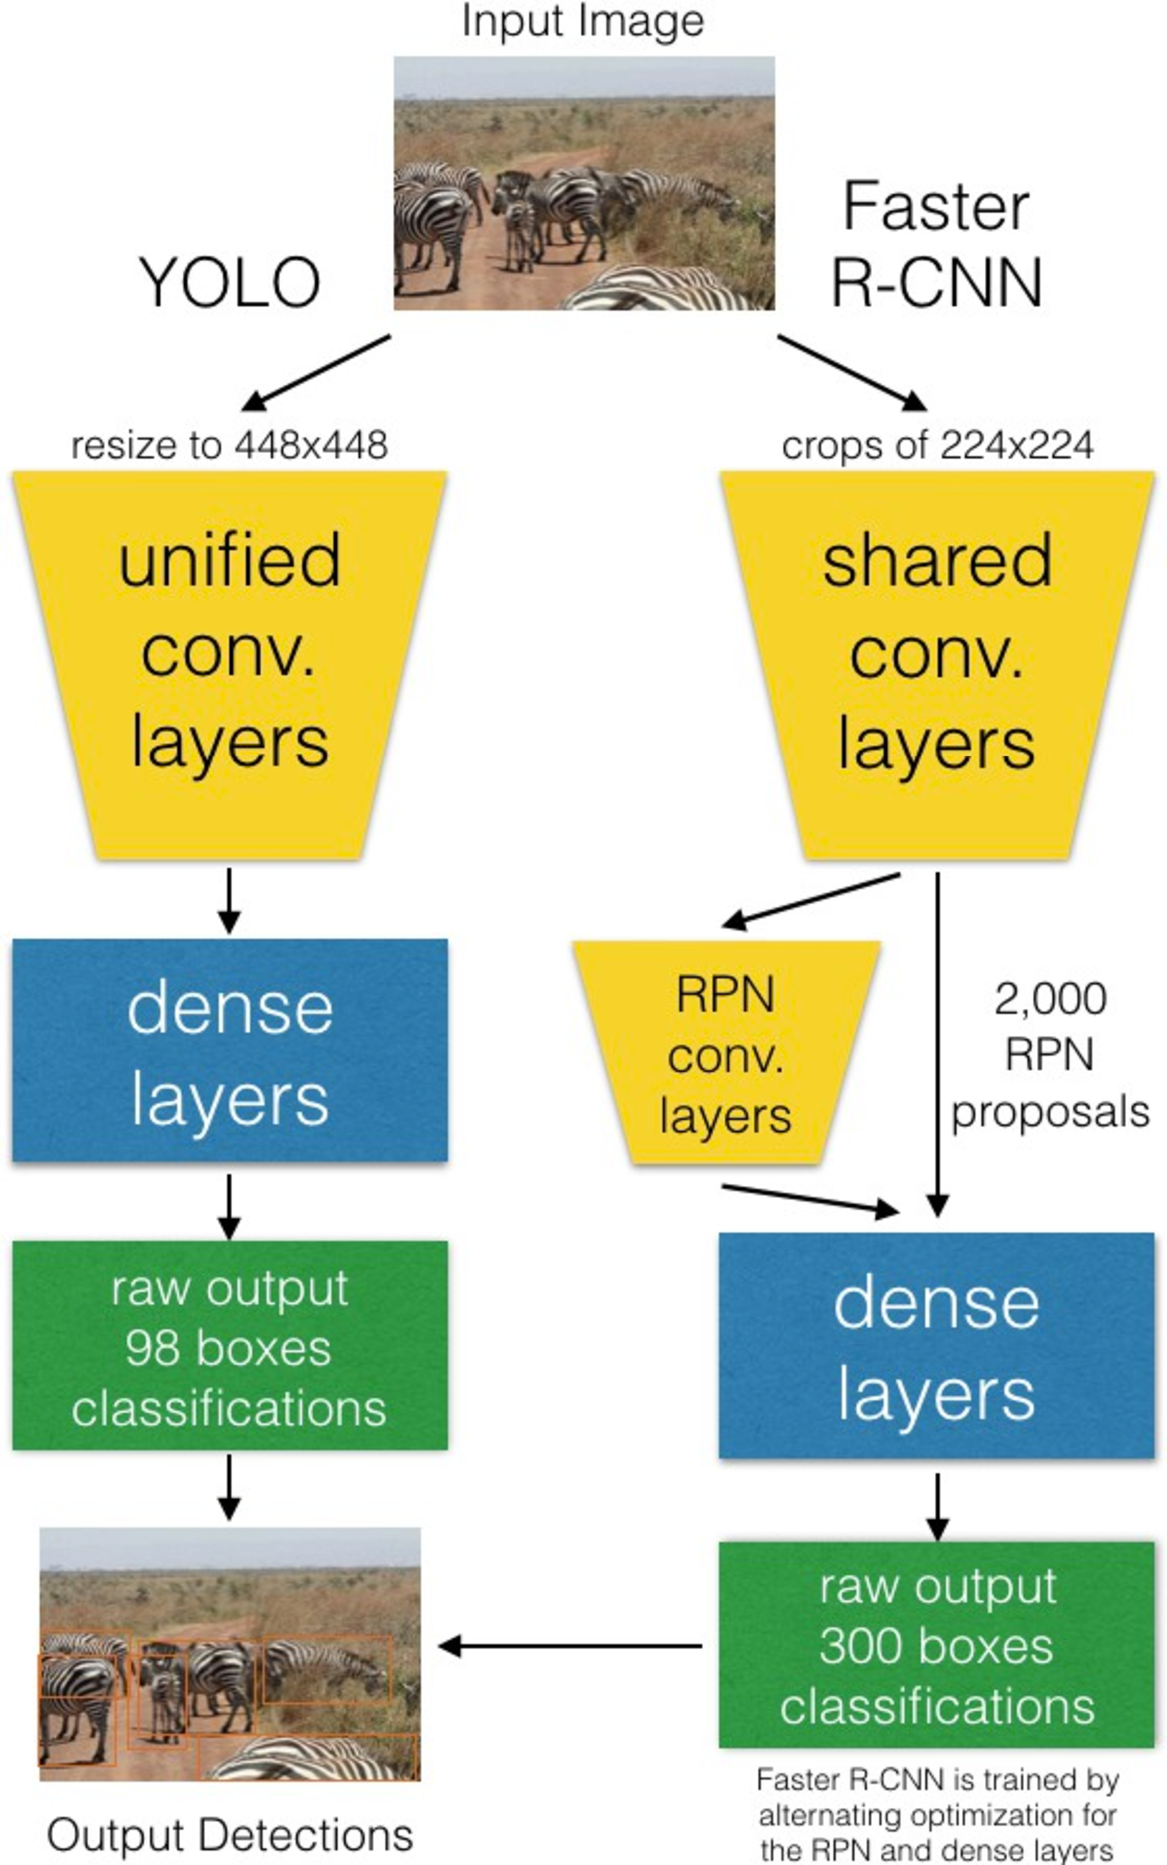
\includegraphics[width=0.58\linewidth]{resources/comparison.pdf}
    \end{center}
    \caption{The YOLO network is a unified architecture that is trained top-to-bottom to minimize bounding box regression and classification error.  In contrast, Faster R-CNN has a separate Region Proposal Network (RPN) that proposes salient object bounding box proposals, which are classified to produce class probabilities.  Faster R-CNN is trained by alternating the training between the RPN and the classification ``networks'' until it converges, applying both gradients to the shared convolutional layers.  \copyright 2016 IEEE. Reprinted, with permission, from: J. Parham and C. Stewart, ``Detecting plains and Grevy’s zebras in the real world,'' in \textit{IEEE Winter Conf. Applicat. Comput. Vis. Workshops}, Lake Placid, NY, USA, Mar. 2016, pp. 1–9.}
    \label{fig:cnncompare}
\end{figure}

During test time, the shared convolutional features are only computed once.  The RPN adds additional convolutional layers on top of the shared filters to generate localization predictions.  The benefit of this architecture is that the training is mostly unified, which dramatically increases speed performance during both training and testing.  Furthermore, replacing Selective Search with the RPN also improves accuracy.  However, the branching top of the network involves additional complexity during training, and the network still does not quite achieve real-time performance on GPUs.  The Faster R-CNN network runs at about six frames-per-second on high-end GPUs but achieves state-of-the-art performance for detection~\cite{russakovsky_imagenet_2015} as of 2016.  The implementation of Faster R-CNN seen in this evaluation is unmodified other than training for 30,000 iterations (with the newer and faster ``end-to-end'' scheme) on different classes. Unfortunately, the training diverged several times before a stable model was produced because the RPN failed to generate valid bounding boxes.

\subsection{You Only Look Once (YOLO)}

The You Only Look Once (YOLO, version 1) network by Redmon \textit{et al.}~\cite{redmon_you_2016} is a variant of single-shot detectors (e.g., SSD~\cite{liu_ssd:_2016}).  Single-shot detectors directly output a fixed-length regression output for a given fixed-sized input image without needing a separate region proposal network (RPN).  Refer to Section~\ref{sec:ssd} for more details.  The architecture of YOLO is somewhat unusual as it uses a relatively large input image (448$\times$448 pixels, compared to its contemporaries that mostly use 224$\times$224 pixels) and produces 98 detection regions from a grid of 7$\times$7 classification cells.  Therefore, the network's output is always 98 bounding box coordinates along with an object score for each of the six species classes from WILD on each bounding box.

The YOLO detector implements a truly unified network architecture.  The network produces multi-class bounding box candidates directly from a single forward inference on an image.  See Figure~\ref{fig:cnncompare} for a high-level comparison between Faster R-CNN and YOLO.  The benefit of a unified integration is most notably speed for the cost of a slight drop in accuracy.  For YOLO, the re-sized training images are given to the network in batches of 64, and the error gradient for each of the 98 network detections is computed directly using the ground-truth bounding boxes, which are mapped onto the range $[0, 1]$.  The entire image is given to the network during test time, which outputs a vector encoding of the 98 bounding box coordinates, a saliency probability for each bounding box, and class probabilities for every 49 (7$\times$7) classification cell. Thus, each 64$\times$64-pixel classification cell contributes two bounding box proposals.  The bounding box saliency probabilities are combined with the corresponding cell's classification probabilities to create the final class probabilities assigned to each bounding box.  The class with the highest probability becomes the bounding box label, and final detections are generated by thresholding the low scoring probabilities and non-maximum suppression.

The YOLO network is trained to optimize a complex, multi-part loss function.  The mathematical definition of the loss function is presented in~\cite{redmon_you_2016}, but -- to summarize it here quickly -- the loss has five components: 1) a regression sum-squared difference loss (SSDL) for each cell's bounding box center x and y pixel, 2) a regression SSDL for the square-root of each bounding box width and height, 3) a conditional SSDL for the saliency probability of whether an object exists in a bounding box, 4) a corresponding conditional SSDL for if an object does \textit{not} exist, and 5) an SSDL for the class probabilities of each cell.~\cite{redmon_you_2016}  To combat training instability, the authors use 1) two weighting hyper-parameters on the regression and classification loss terms to balance their respective error gradients, and 2) a unique learning rate schedule (called ``burn-in'') that starts intentionally very slow, then increases around iteration 600 for routine training.

YOLO V2 (version 2)~\cite{redmon_yolo9000:_2016} includes specific improvements to increase the network's ability to detect small objects more accurately.  The network includes training improvements like batch normalization~\cite{ioffe_batch_2015}, multi-scale training and model improvements like anchor boxes, direct bounding box regression (instead of predicting residuals), is fully convolutional, and has a higher-resolution convolutional output.  While these improvements helped stabilize training, the network still diverged several times before a stable random initialization was chosen and the model converged (trained for 24,000 iterations).  Since YOLO V2 consistently outperforms YOLO v1, we do not report it in this evaluation and focus on comparing the detection performance of Hough Forests, Faster R-CNN, and YOLO v2.

\subsubsection{Performance Trade-Offs}

The YOLO network has distinct advantages over Hough Forests: 1) it has significantly more parameters to fit the training data, 2) has a larger effective receptive field for better regression performance, 3) uses convolutional feature extraction with transfer learning on ILSVRC, and 4) is inherently multi-class.  In comparison to Faster R-CNN, YOLO achieves real-time performance and, as mentioned previously, simplifies the entire detection pipeline down to a single forward inference.  However, YOLO is more difficult to train with its poorly-behaving error gradient and has several network-specific hyper-parameters.  Like Faster R-CNN, the YOLO network (realistically) requires a GPU to train, and both take significantly longer to train over Hough Forests.  Both neural networks were trained for about 24 hours using two Titan X GPUs, whereas the ensemble of 10 Hough Forests trees was trained in just under 3 hours on a quad-core CPU.  That being said, the testing speeds of both neural networks are at least two orders of magnitude faster compared to the Hough Forests implementation, which runs at roughly 15 seconds per image for nine scales.

On top of training speed advantages, the Hough Forests implementation does not require nearly as much training data.  Furthermore, the convolutional filters of each neural network are initialized with pre-trained weights~\cite{oquab_learning_2014} before fine-tuning on the dataset.  Between the two deep learning detectors, the YOLO network utilizes empty images (images with no ground-truth bounding boxes of any species) during training with implicit negative mining, whereas Faster R-CNN was not.  This training procedure allows YOLO to see slightly more images during training, which represents 1.7\% of the dataset (see Figure~\ref{fig:densities}, density 0).

\subsection{Results}

\begin{table}[!t]
    \caption{The number of correct detections and incorrect detections for two failure modes (localization and classification) of each algorithm, combined for both species.  Localization errors fail to put a bounding box around an animal, while classification errors have a correct box but the wrong species label.  The YOLO network gets the highest number of correct detections but has significantly more classification errors than Faster R-CNN.  Faster R-CNN, while it makes more localization errors, seldom guesses the incorrect species.  There are 1,343 test ground-truth detections (714 of plains, 536 of Gr\'evy's, and 93 unspecified).  \copyright 2016 IEEE. Reprinted, with permission, from: J. Parham and C. Stewart, ``Detecting plains and Grevy’s zebras in the real world,'' in \textit{IEEE Winter Conf. Applicat. Comput. Vis. Workshops}, Lake Placid, NY, USA, Mar. 2016, pp. 1–9.}
    \label{tab:errors}
    \begin{center}
        \begin{tabular}{r|rrr}
            \hline
            \textbf{Algorithm}     & \textbf{Localization Errors} & \textbf{Classification Errors} & \textbf{Correct} \\
            \hline
            \texttt{Hough Forests} & 59.6\%                       & \textbf{0.2\%}                 & 40.2\%           \\
            \texttt{Faster R-CNN}  & 47.8\%                       & 0.5\%                          & 51.7\%           \\
            \texttt{YOLO v2}       & \textbf{31.0\%}              & 13.0\%                         & \textbf{56.0\%}
        \end{tabular}
    \end{center}
\end{table}

\begin{figure}[!t]
    \begin{center}
        \begin{tabular}{cccccc}

            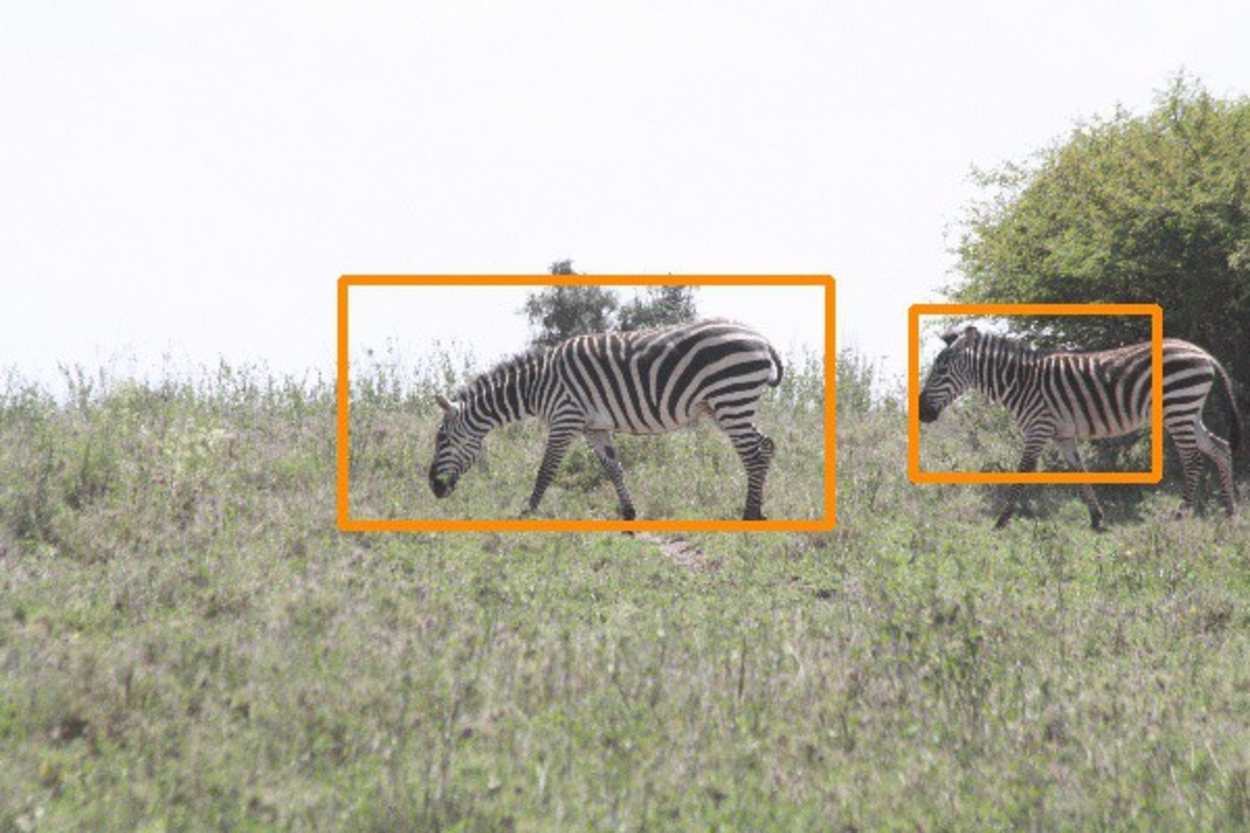
\includegraphics[width=0.13\textwidth]{resources/detections-rf-pz0.pdf}   &
            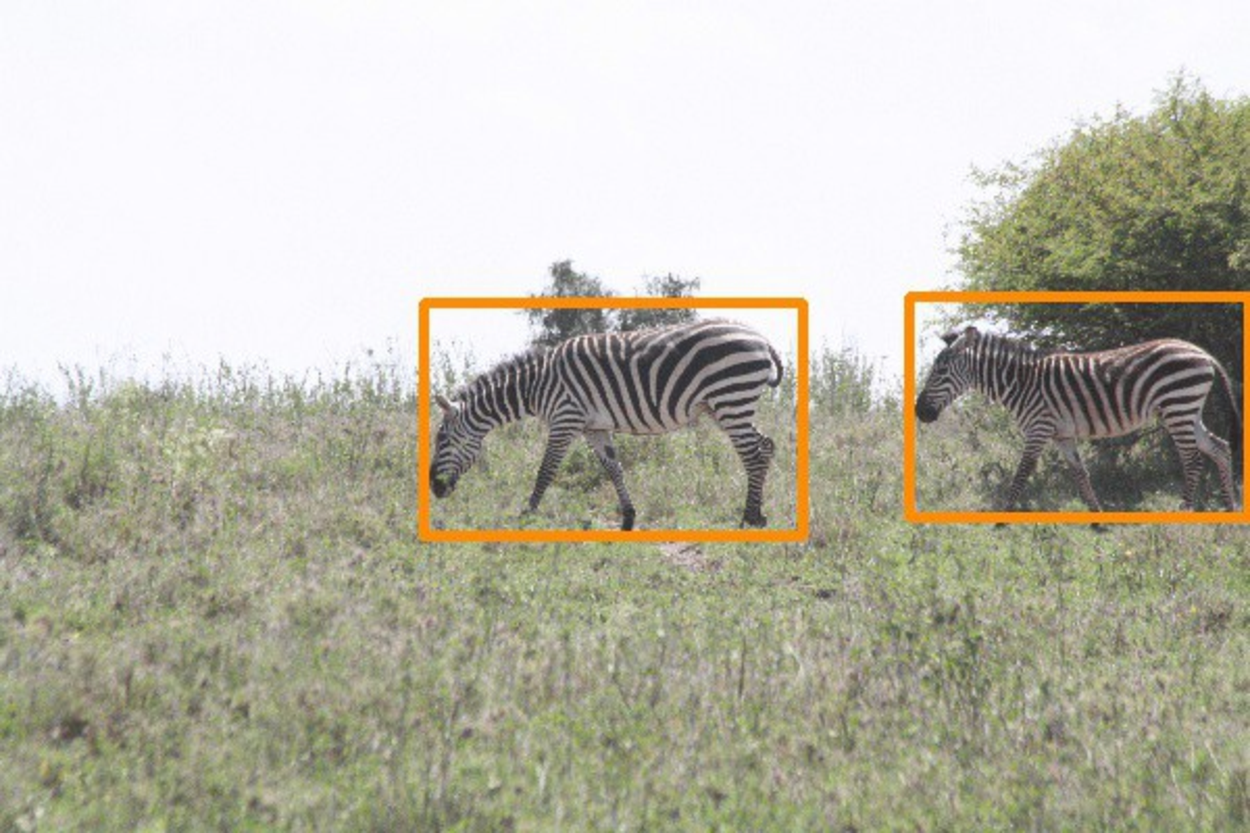
\includegraphics[width=0.13\textwidth]{resources/detections-rcnn-pz0.pdf} &
            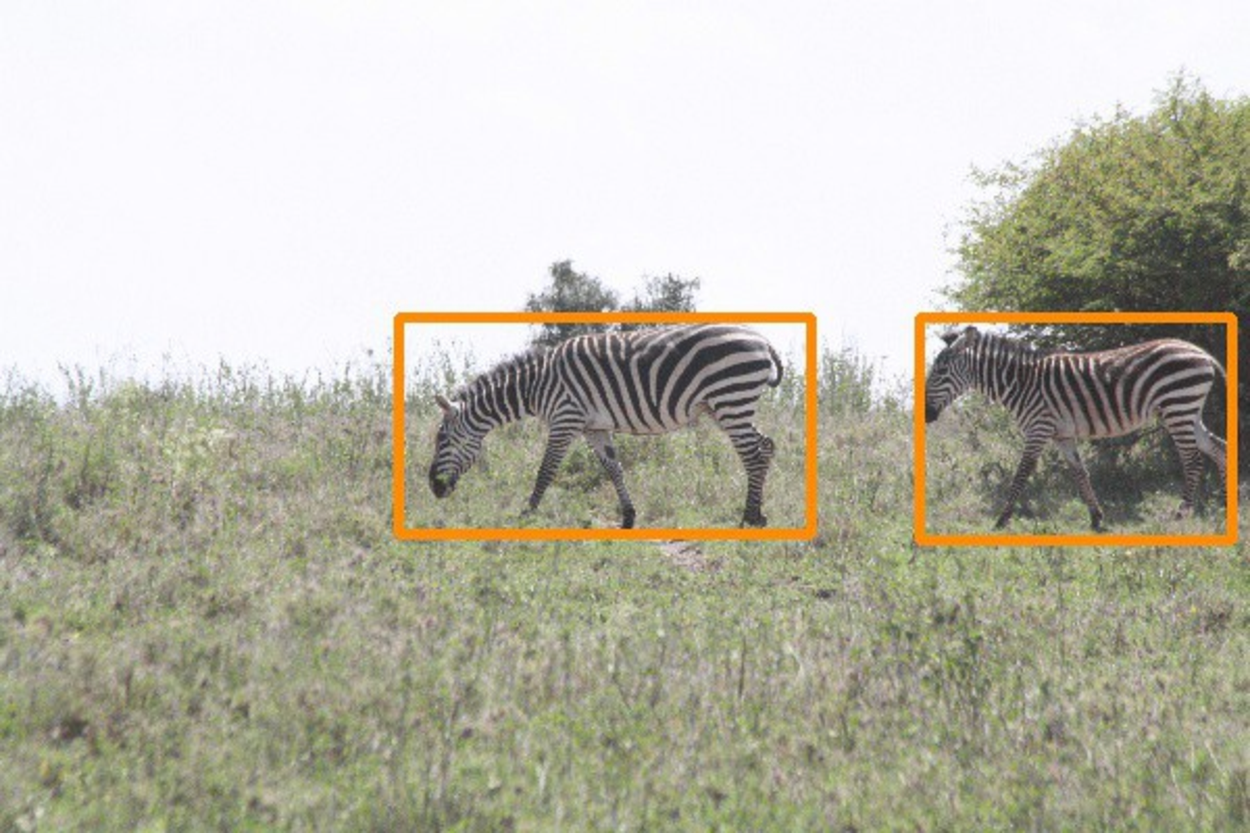
\includegraphics[width=0.13\textwidth]{resources/detections-yolo-pz0.pdf} &
            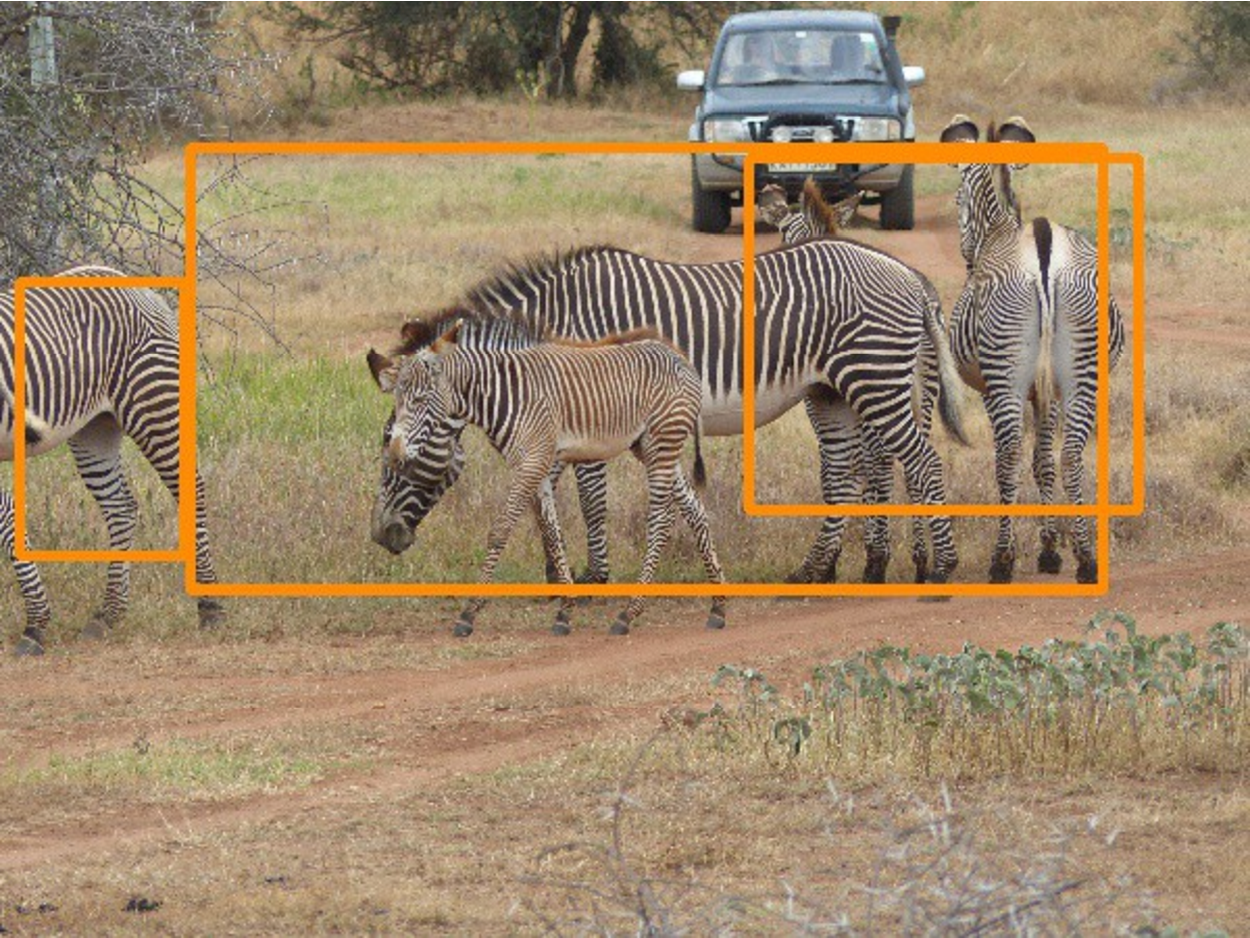
\includegraphics[width=0.13\textwidth]{resources/detections-rf-gz0.pdf}   &
            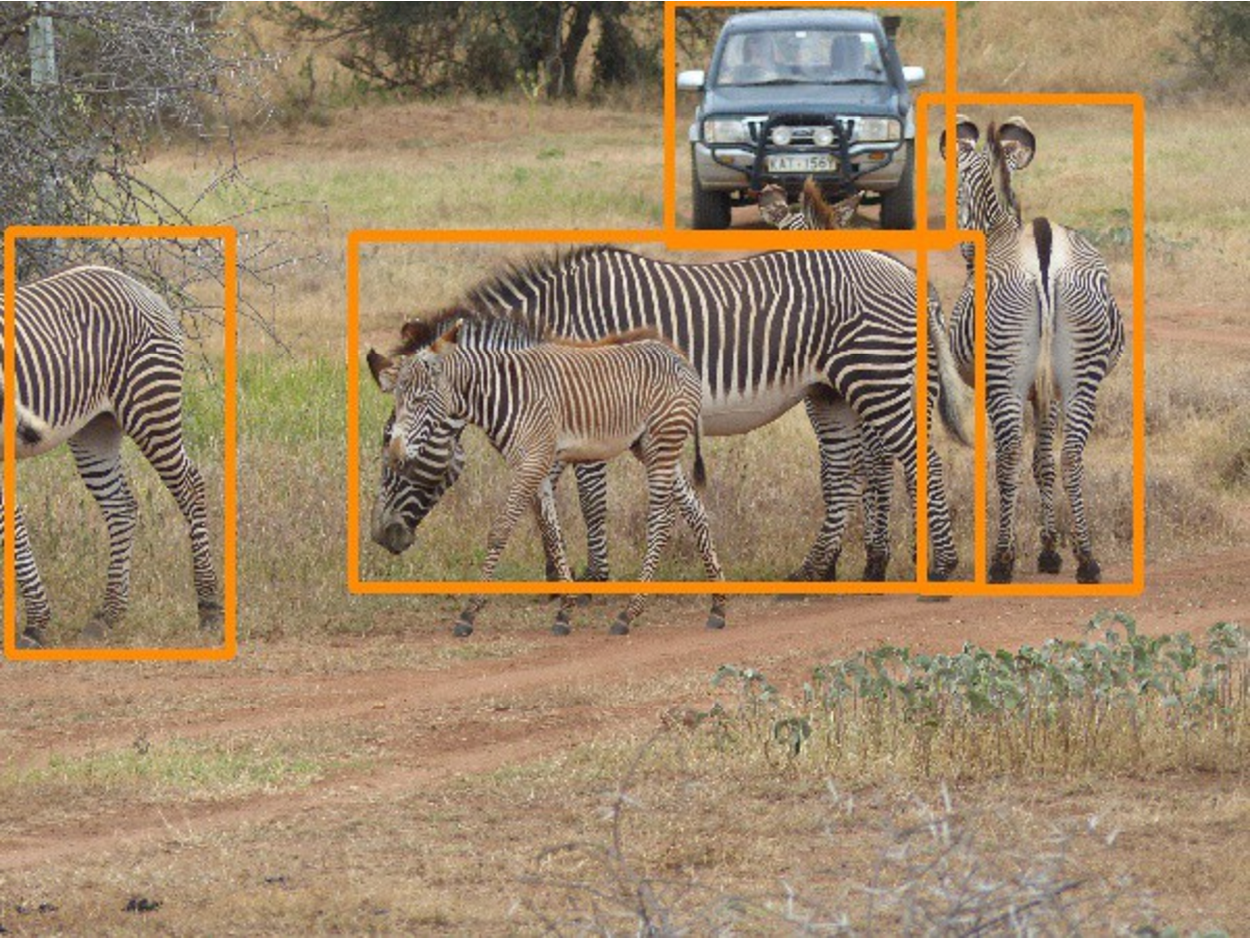
\includegraphics[width=0.13\textwidth]{resources/detections-rcnn-gz0.pdf} &
            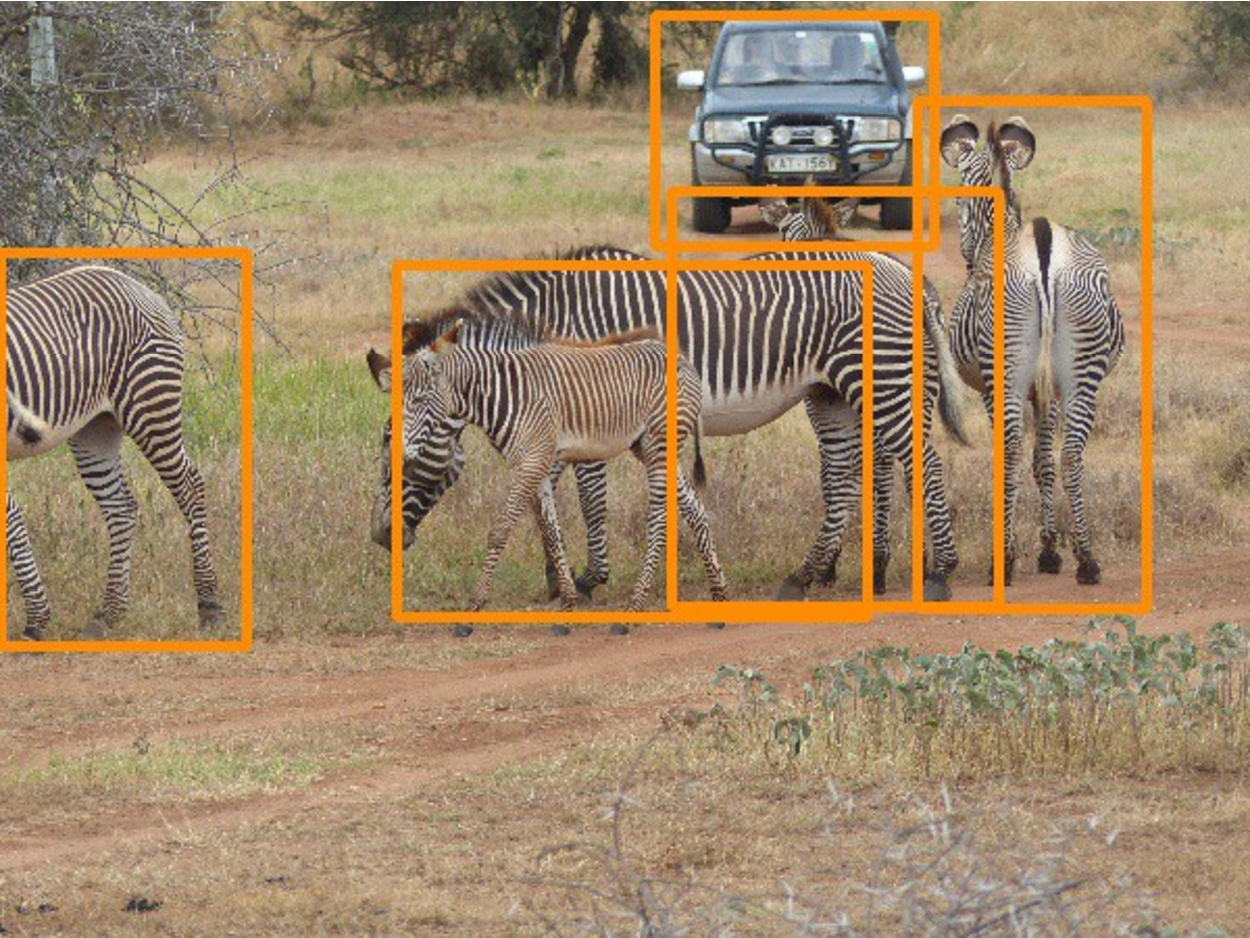
\includegraphics[width=0.13\textwidth]{resources/detections-yolo-gz0.pdf}   \\

            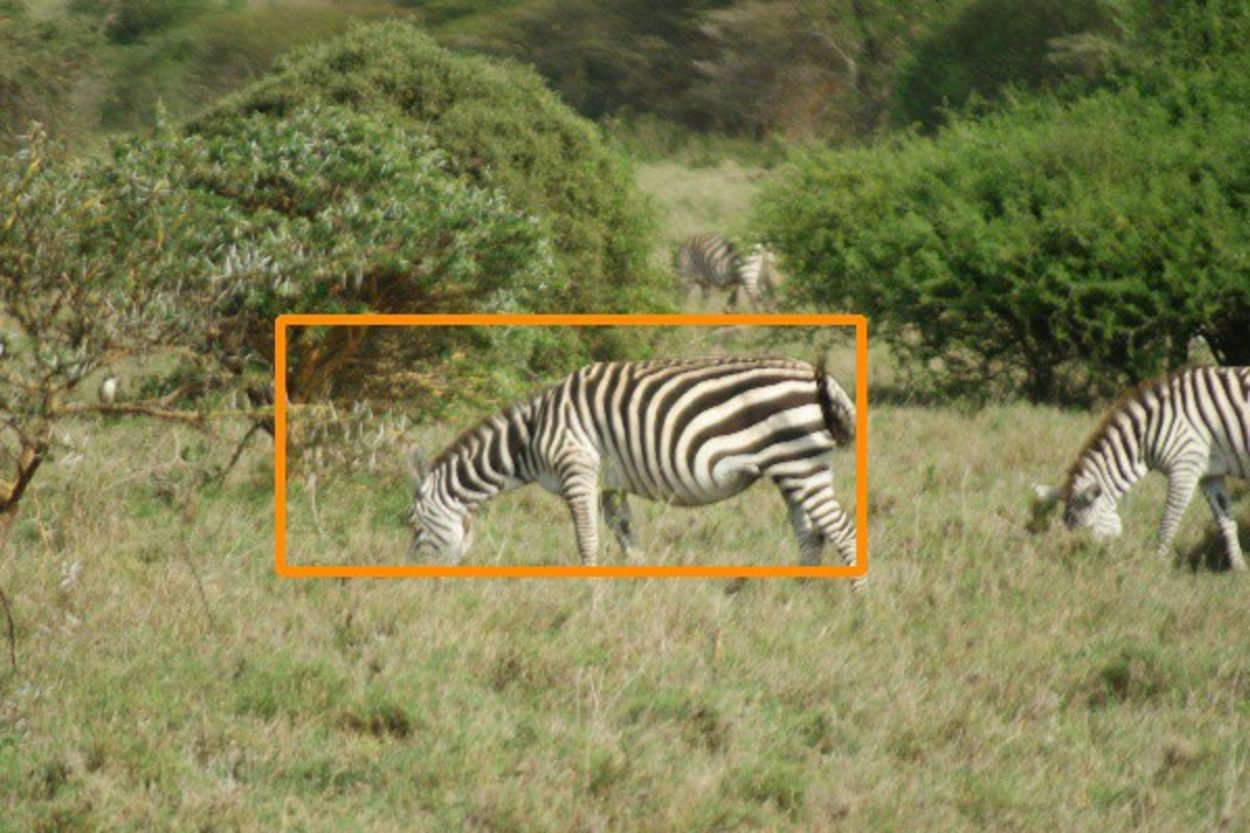
\includegraphics[width=0.13\textwidth]{resources/detections-rf-pz1.pdf}   &
            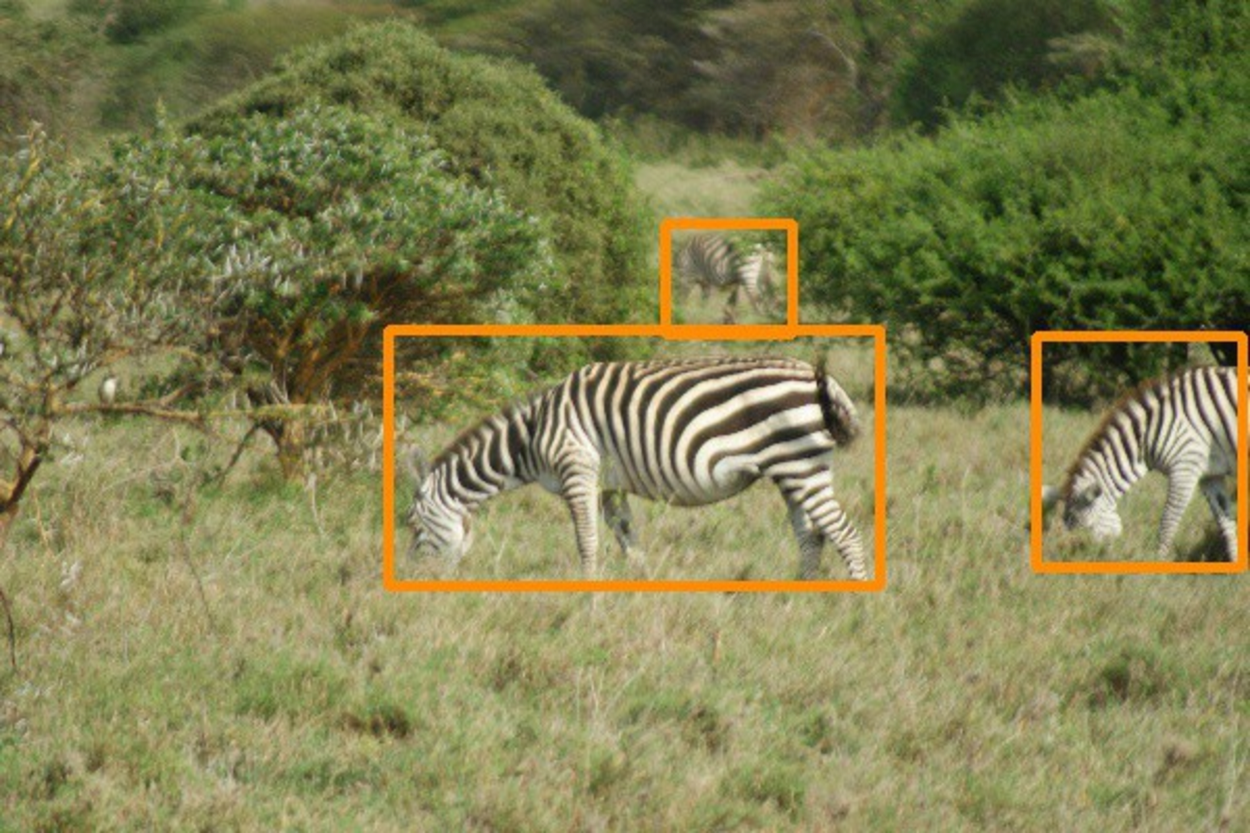
\includegraphics[width=0.13\textwidth]{resources/detections-rcnn-pz1.pdf} &
            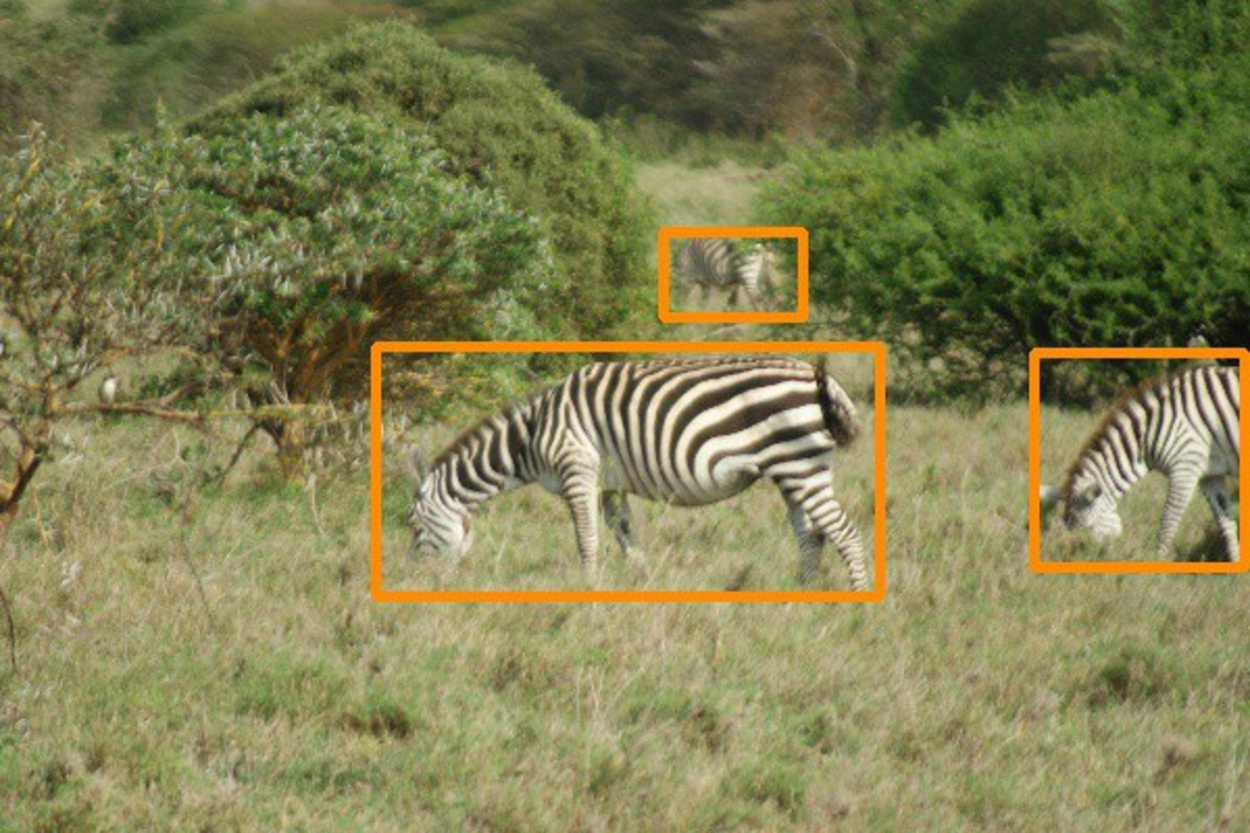
\includegraphics[width=0.13\textwidth]{resources/detections-yolo-pz1.pdf} &
            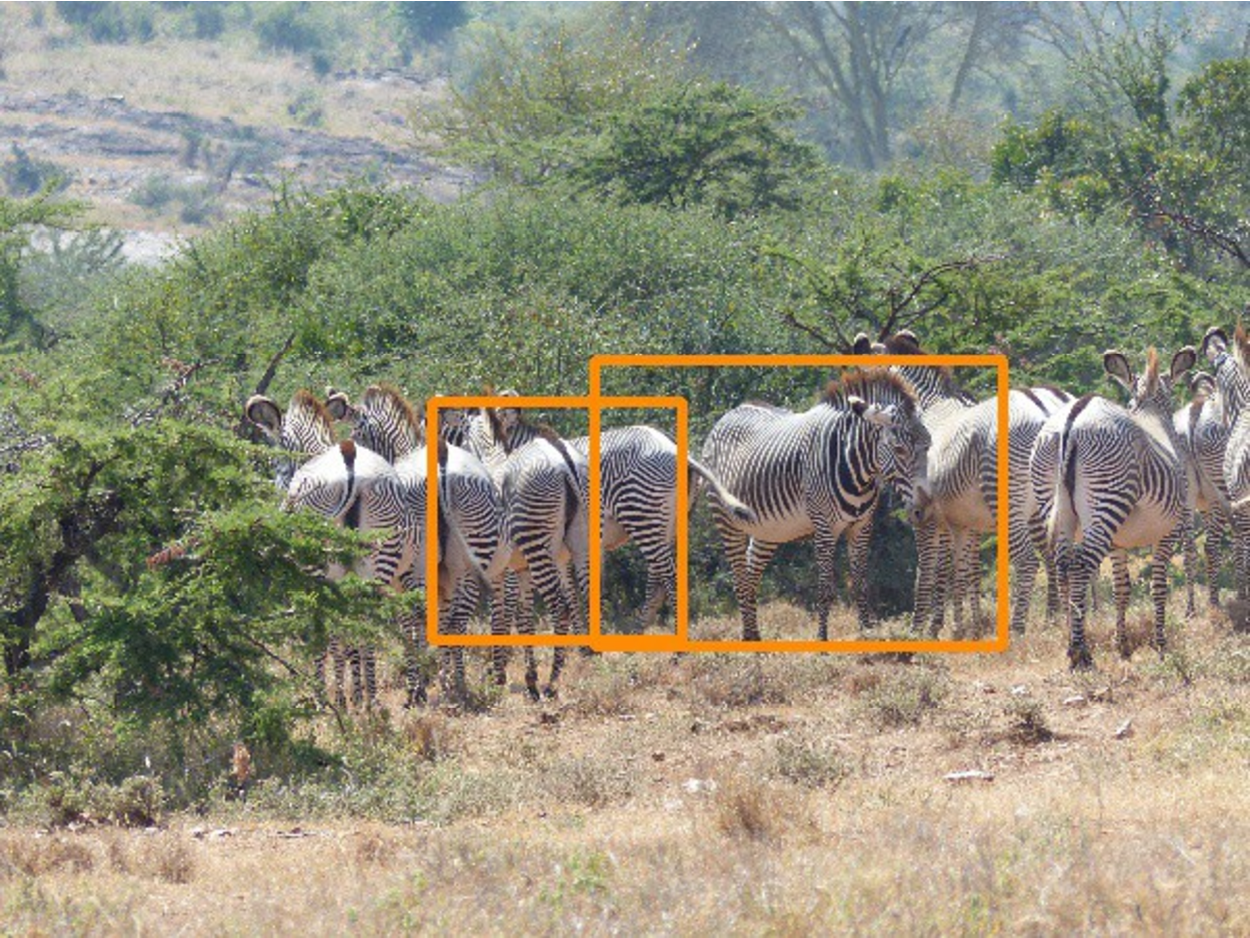
\includegraphics[width=0.13\textwidth]{resources/detections-rf-gz1.pdf}   &
            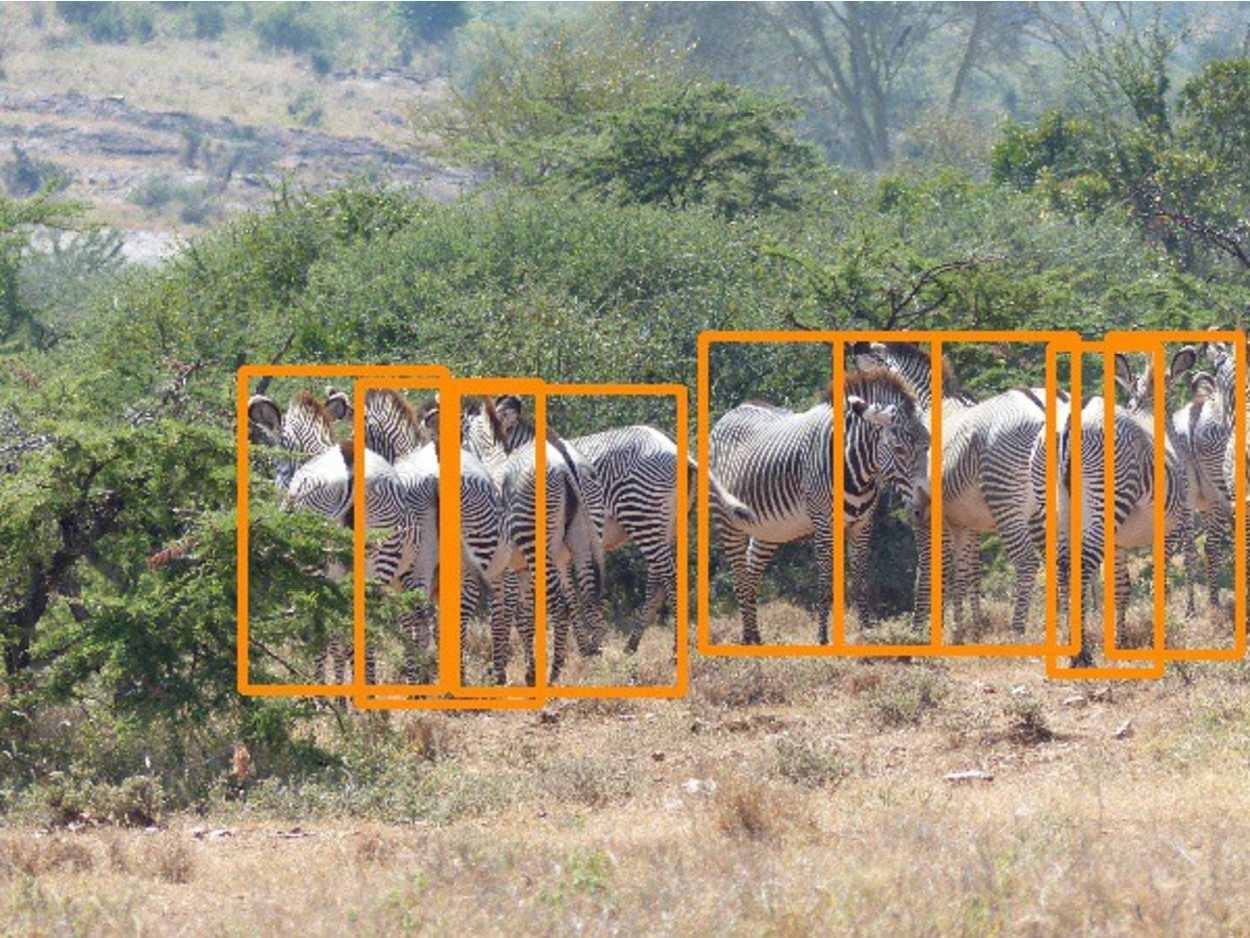
\includegraphics[width=0.13\textwidth]{resources/detections-rcnn-gz1.pdf} &
            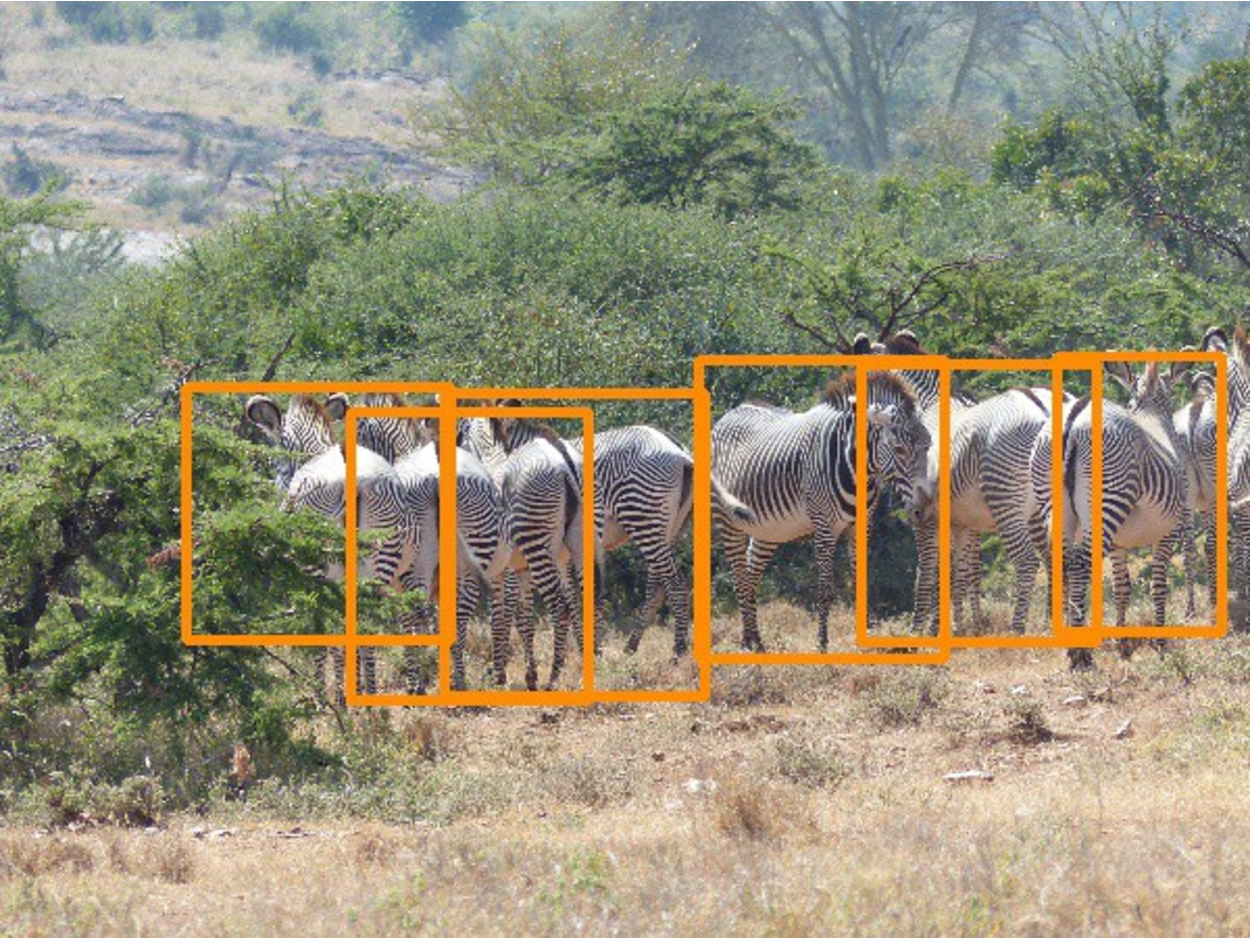
\includegraphics[width=0.13\textwidth]{resources/detections-yolo-gz1.pdf}   \\

            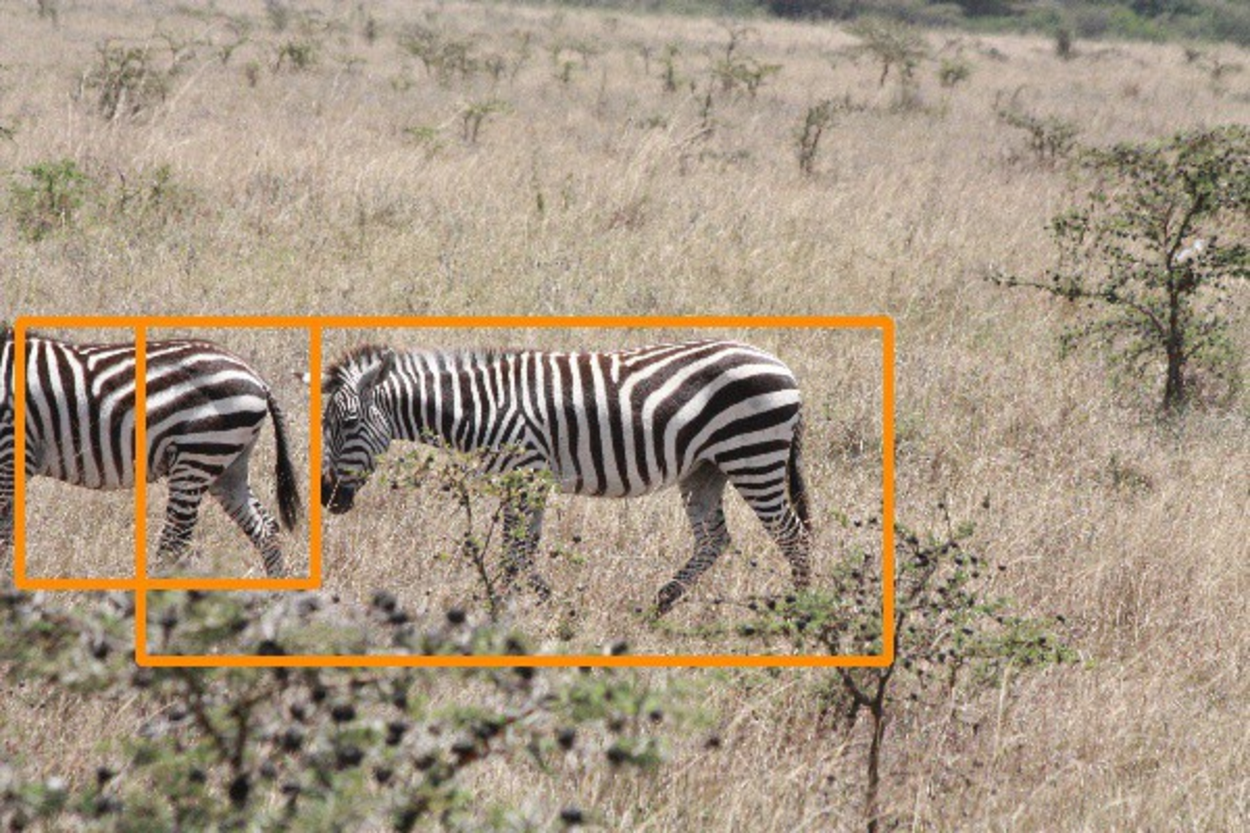
\includegraphics[width=0.13\textwidth]{resources/detections-rf-pz2.pdf}   &
            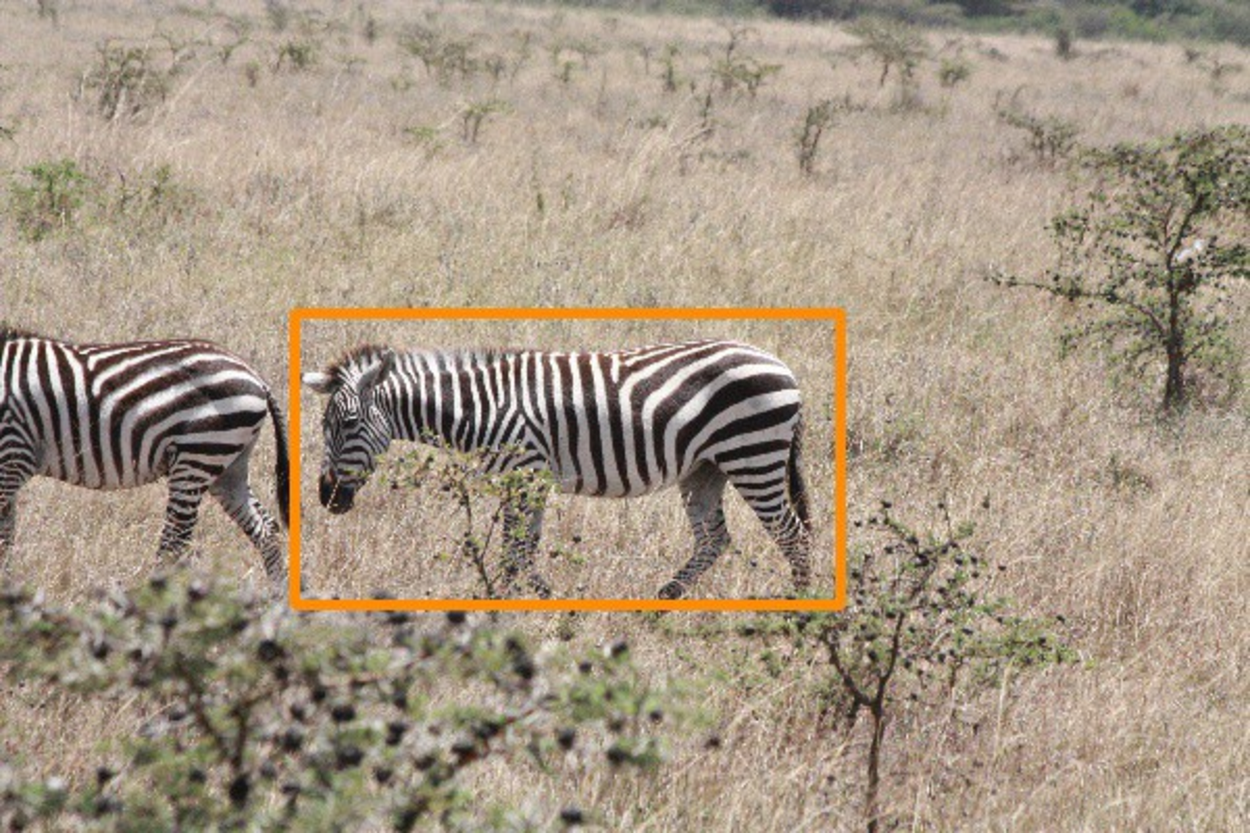
\includegraphics[width=0.13\textwidth]{resources/detections-rcnn-pz2.pdf} &
            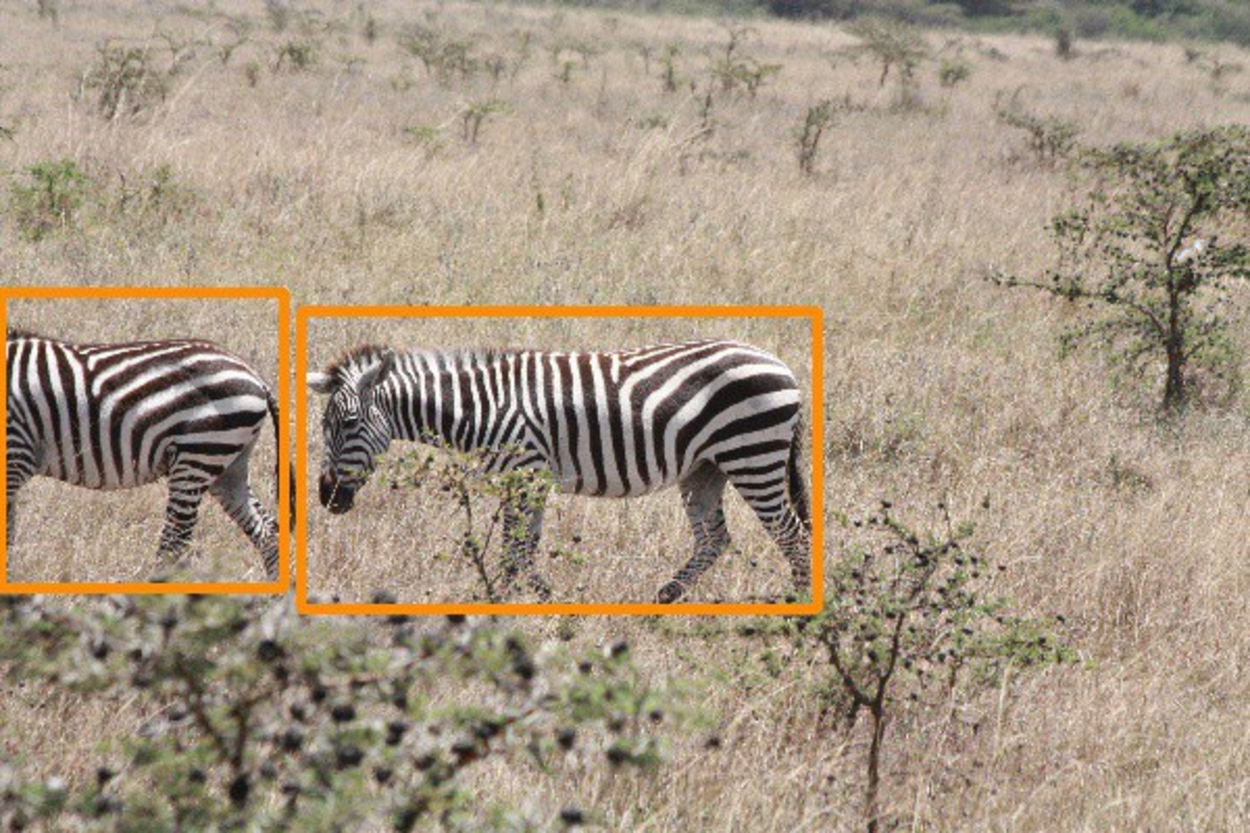
\includegraphics[width=0.13\textwidth]{resources/detections-yolo-pz2.pdf} &
            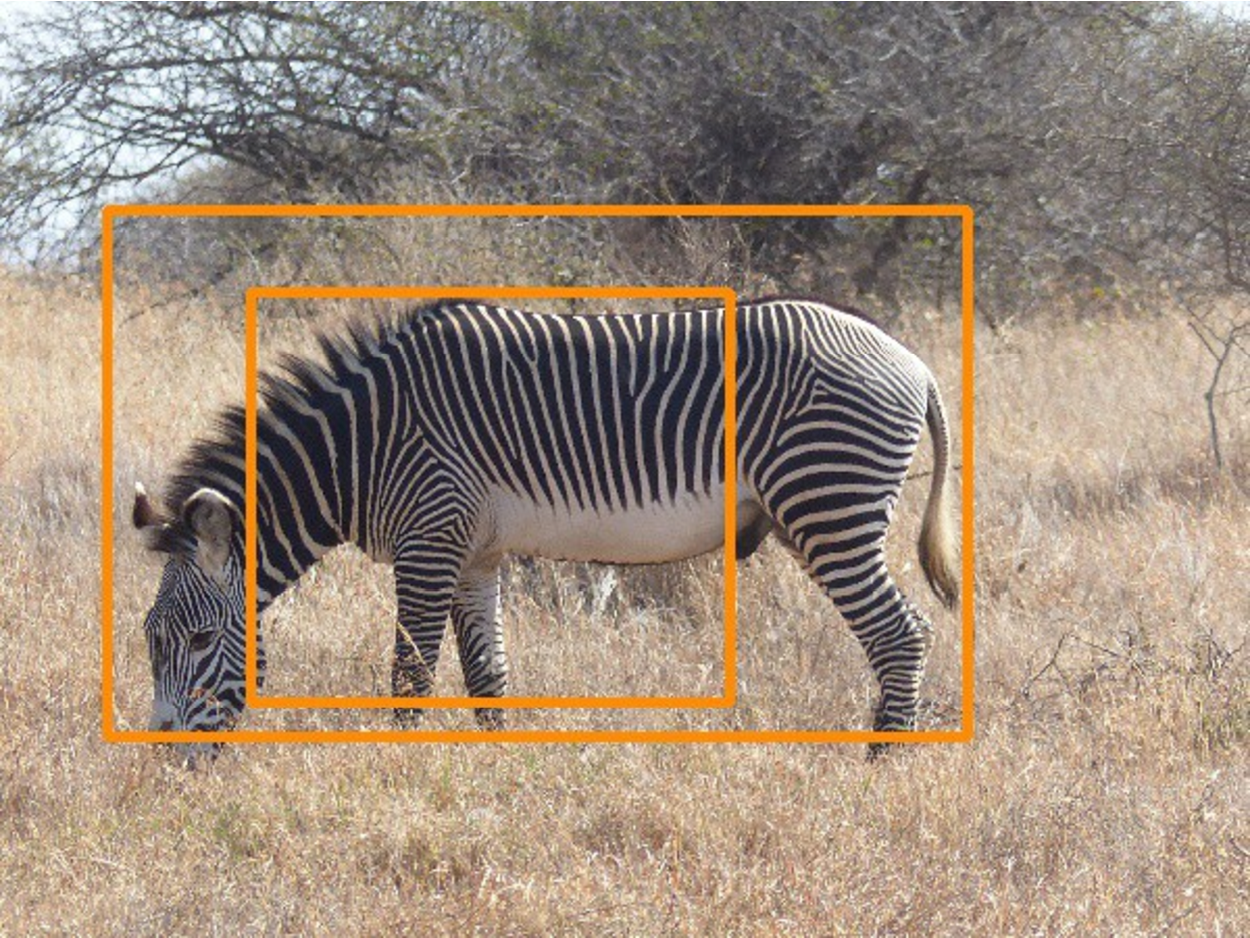
\includegraphics[width=0.13\textwidth]{resources/detections-rf-gz2.pdf}   &
            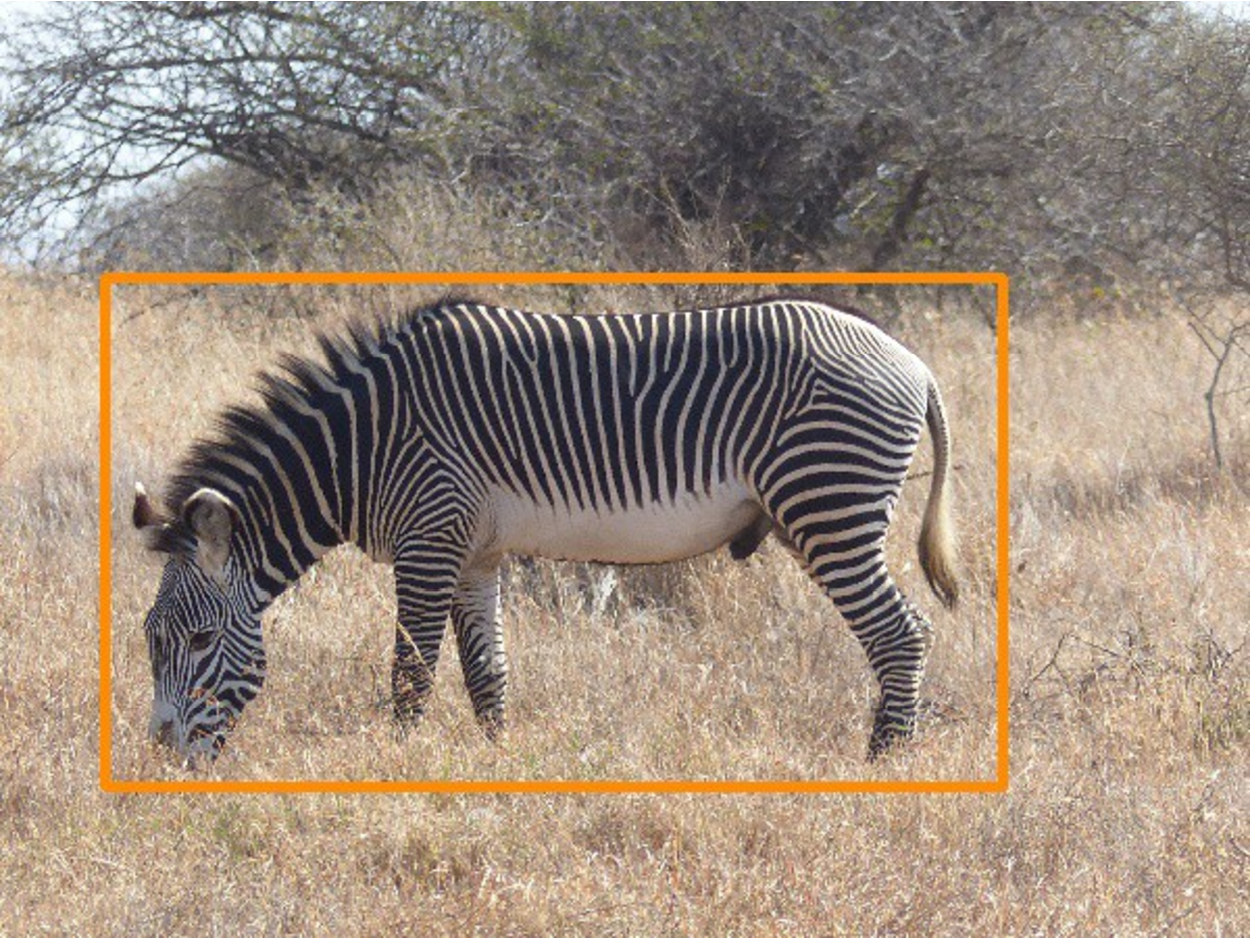
\includegraphics[width=0.13\textwidth]{resources/detections-rcnn-gz2.pdf} &
            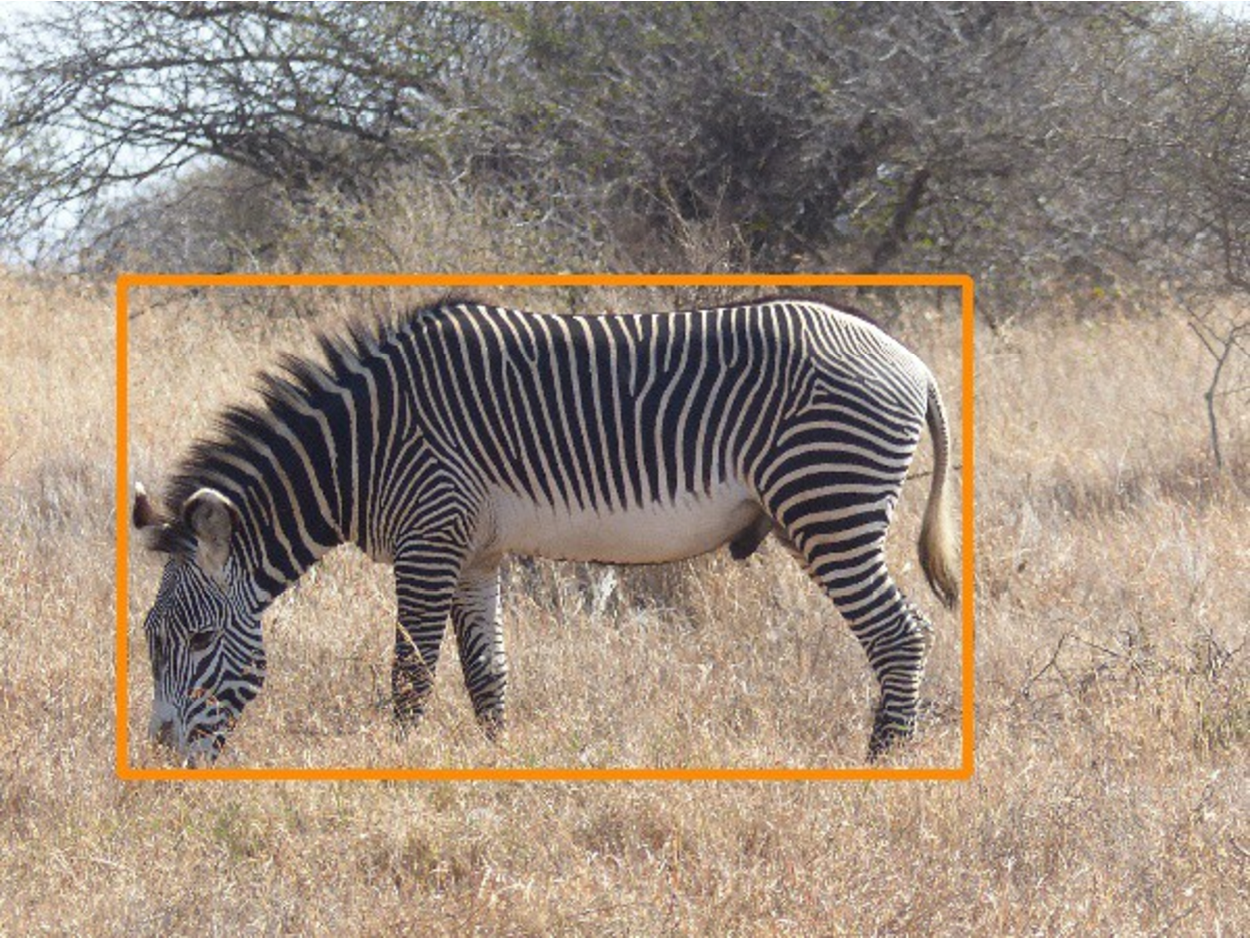
\includegraphics[width=0.13\textwidth]{resources/detections-yolo-gz2.pdf}   \\

            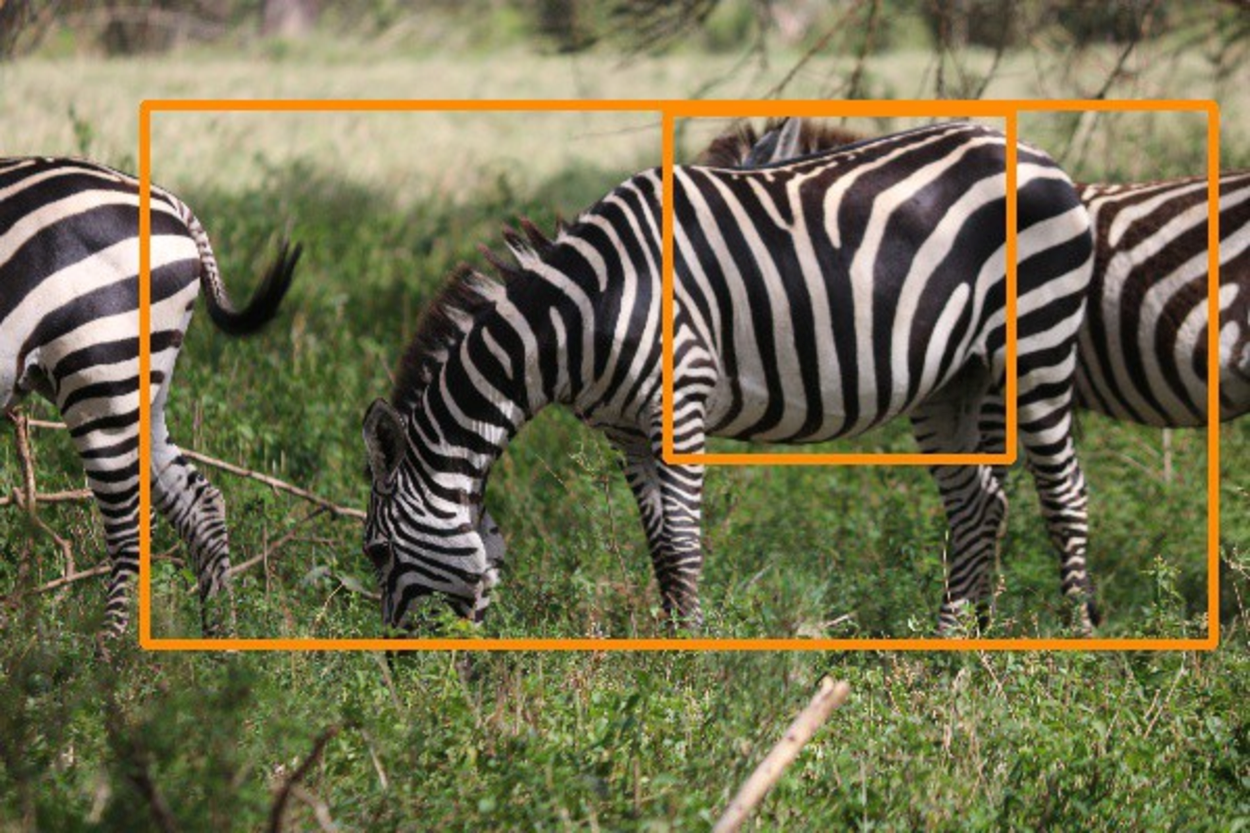
\includegraphics[width=0.13\textwidth]{resources/detections-rf-pz3.pdf}   &
            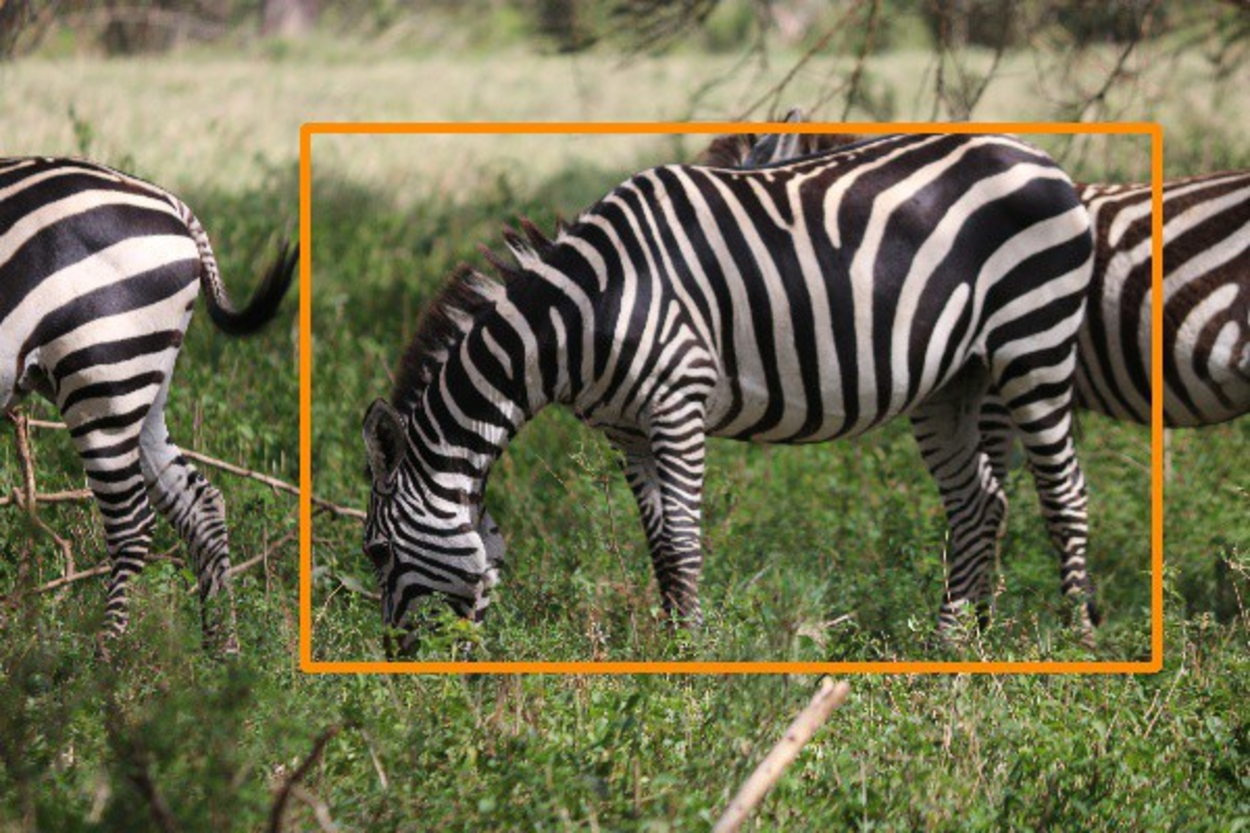
\includegraphics[width=0.13\textwidth]{resources/detections-rcnn-pz3.pdf} &
            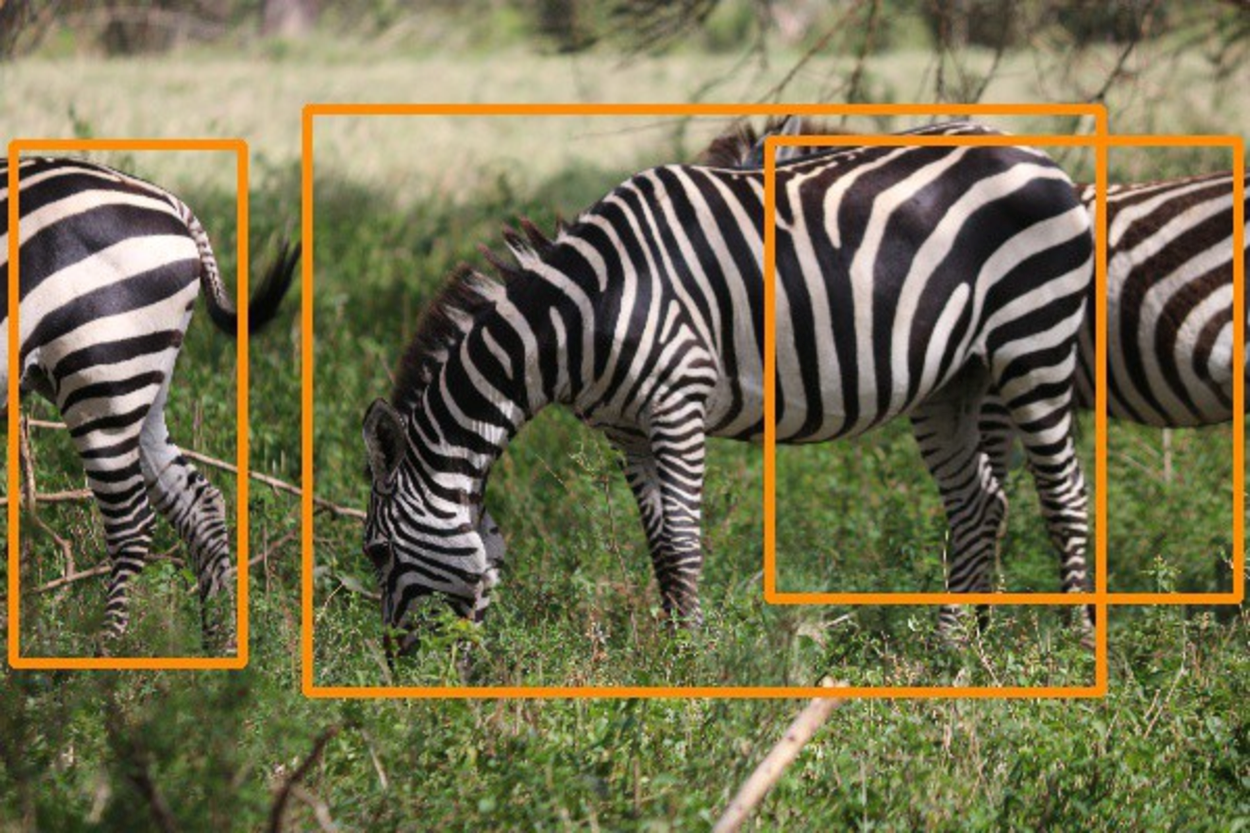
\includegraphics[width=0.13\textwidth]{resources/detections-yolo-pz3.pdf} &
            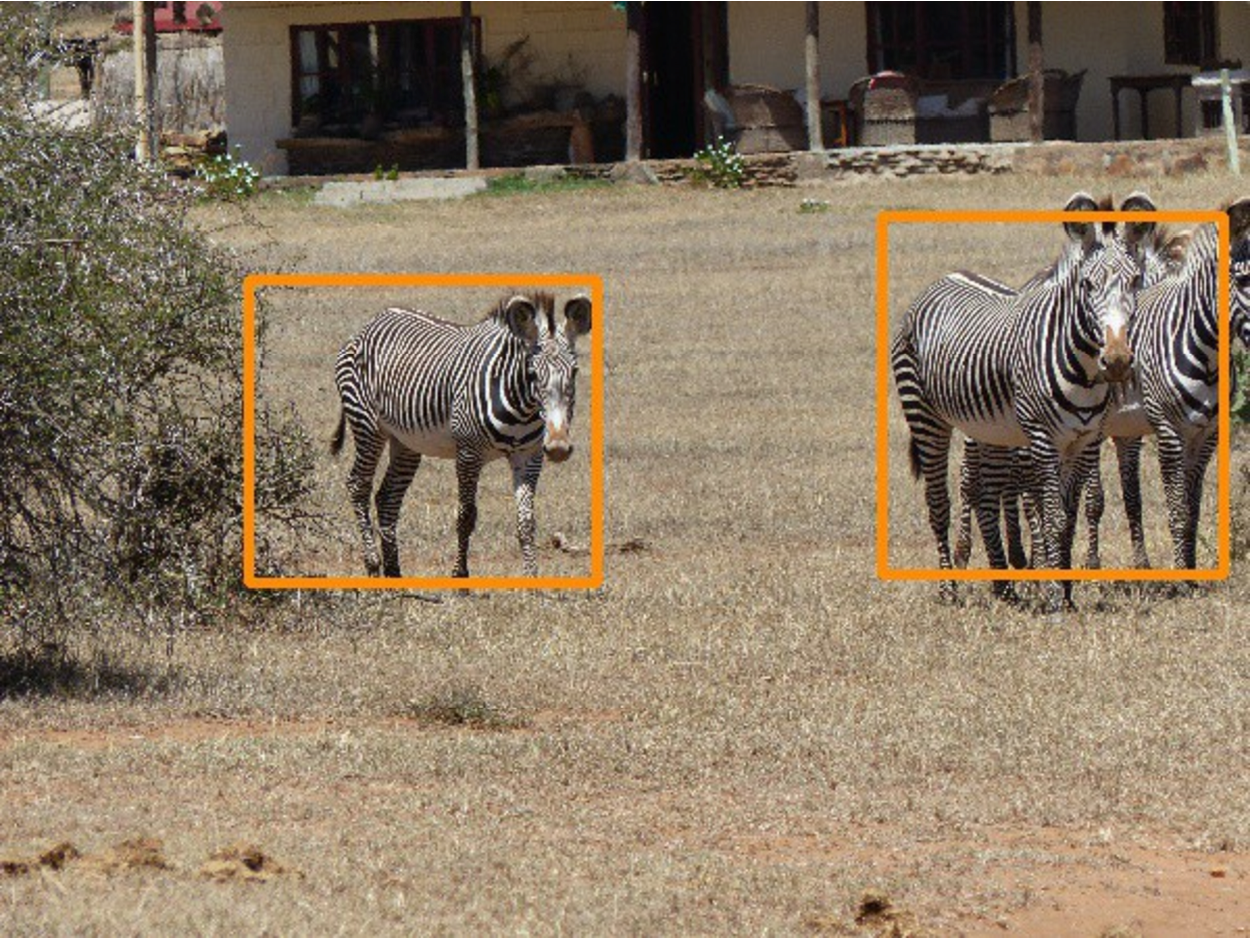
\includegraphics[width=0.13\textwidth]{resources/detections-rf-gz3.pdf}   &
            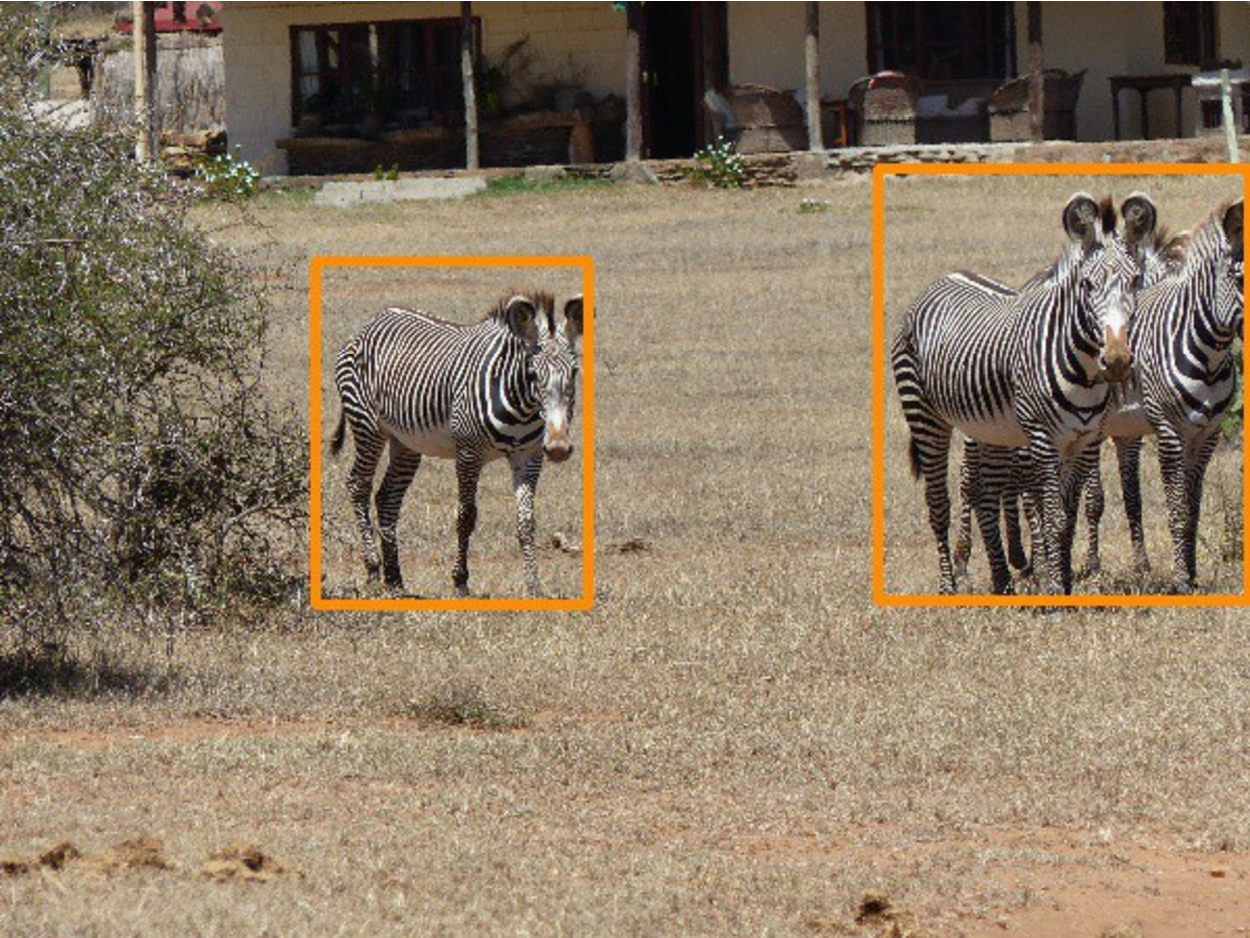
\includegraphics[width=0.13\textwidth]{resources/detections-rcnn-gz3.pdf} &
            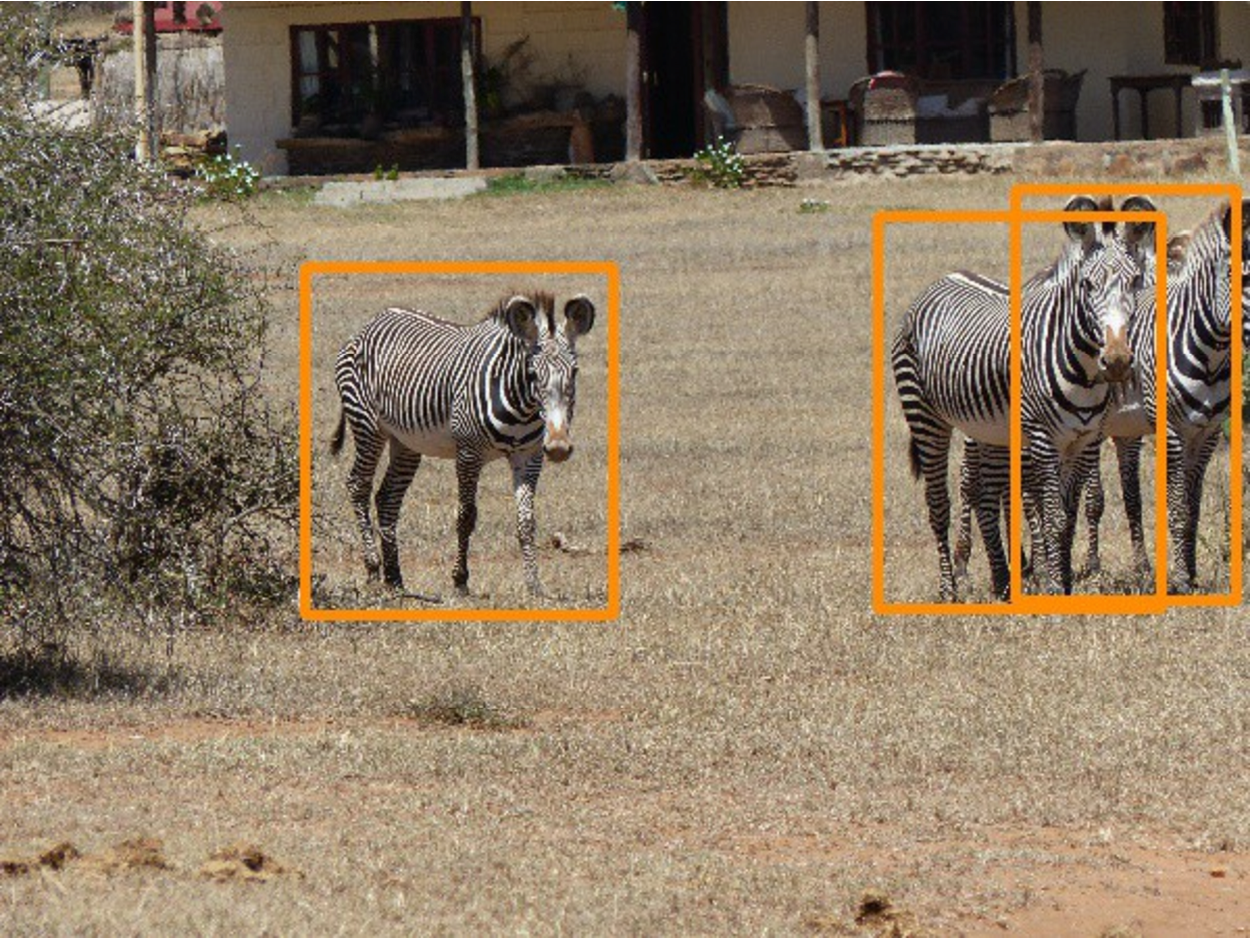
\includegraphics[width=0.13\textwidth]{resources/detections-yolo-gz3.pdf}   \\

            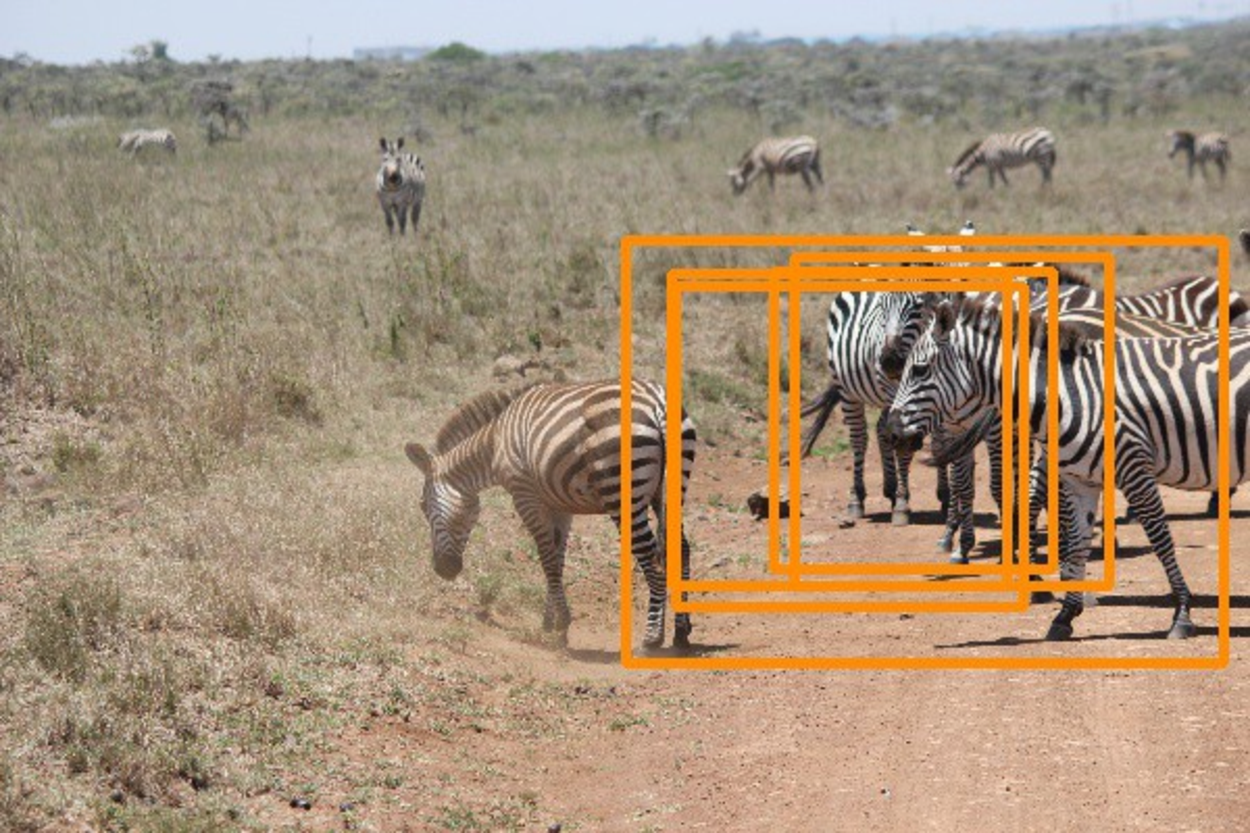
\includegraphics[width=0.13\textwidth]{resources/detections-rf-pz4.pdf}   &
            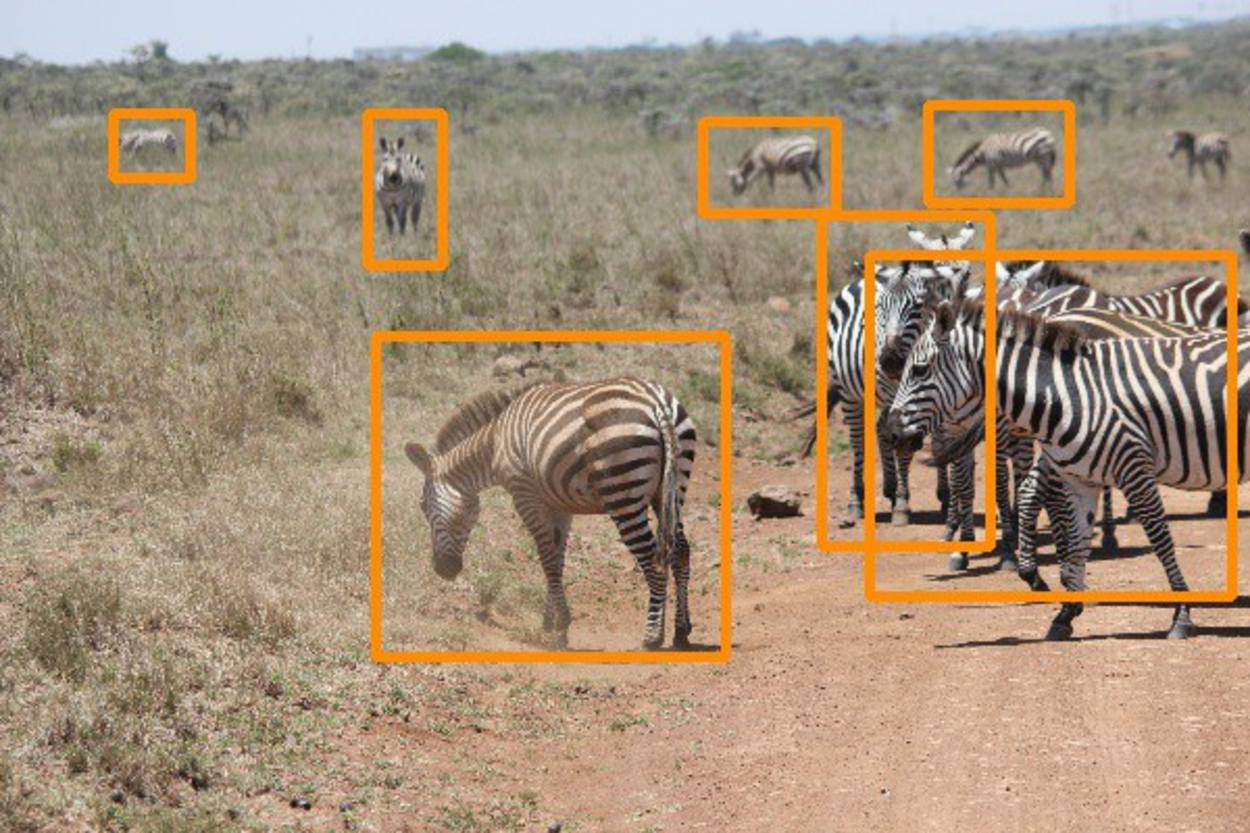
\includegraphics[width=0.13\textwidth]{resources/detections-rcnn-pz4.pdf} &
            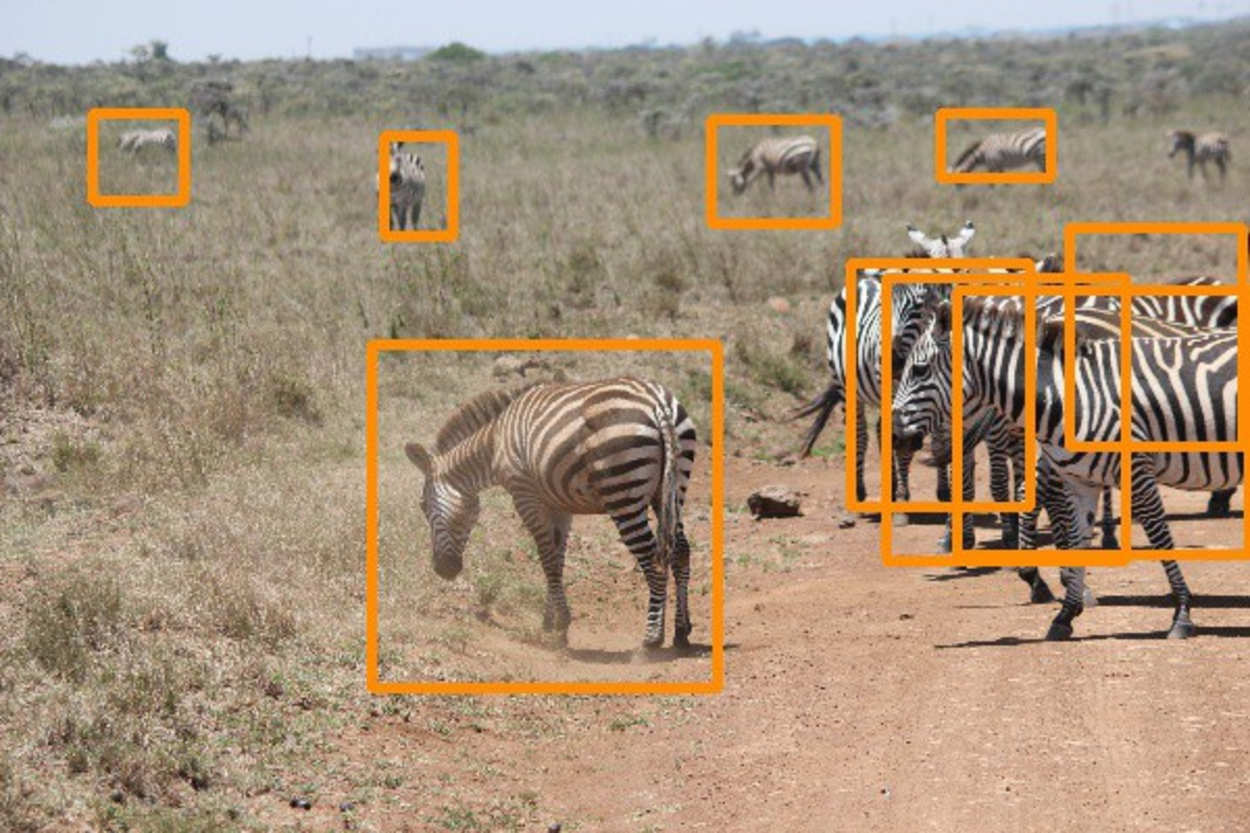
\includegraphics[width=0.13\textwidth]{resources/detections-yolo-pz4.pdf} &
            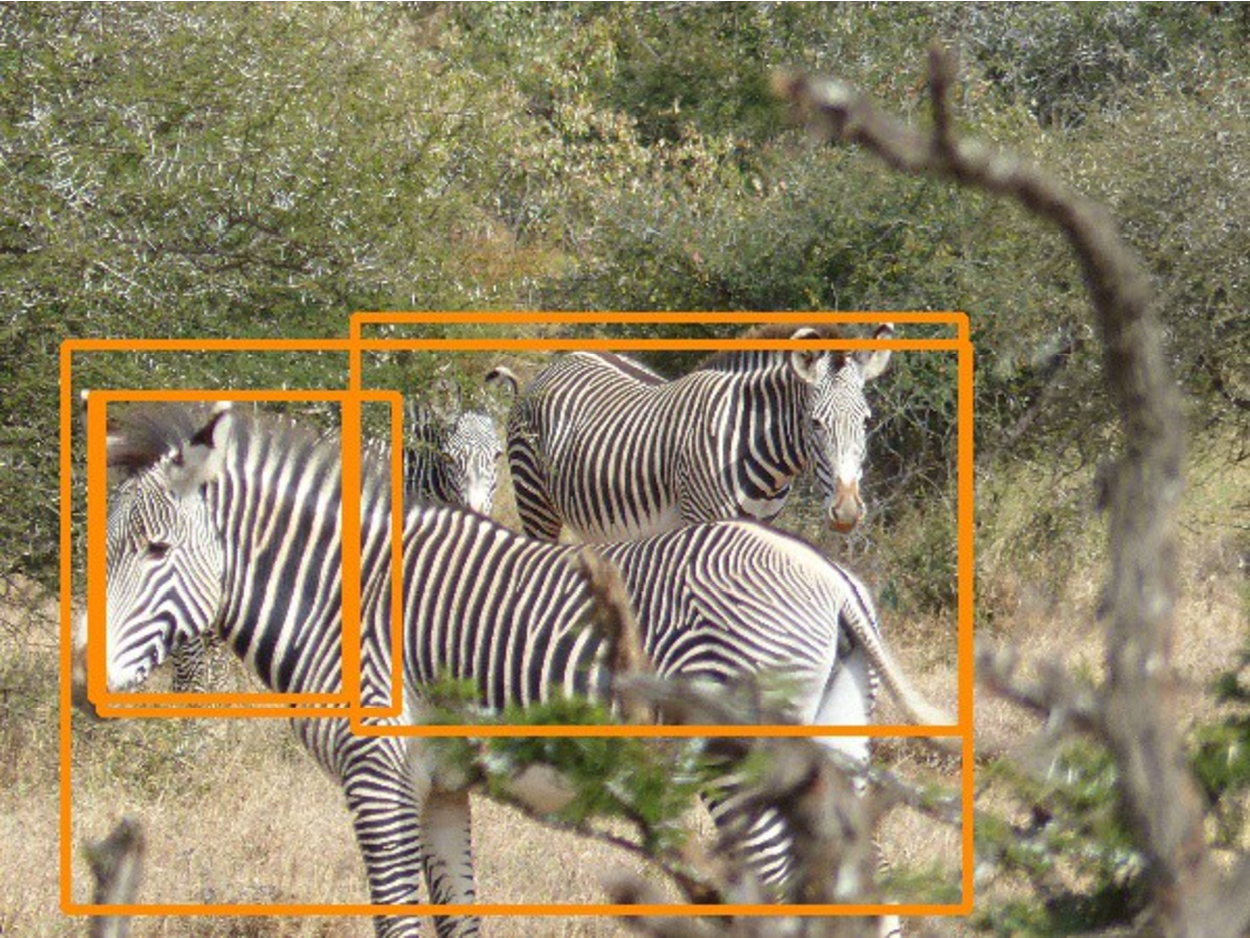
\includegraphics[width=0.13\textwidth]{resources/detections-rf-gz4.pdf}   &
            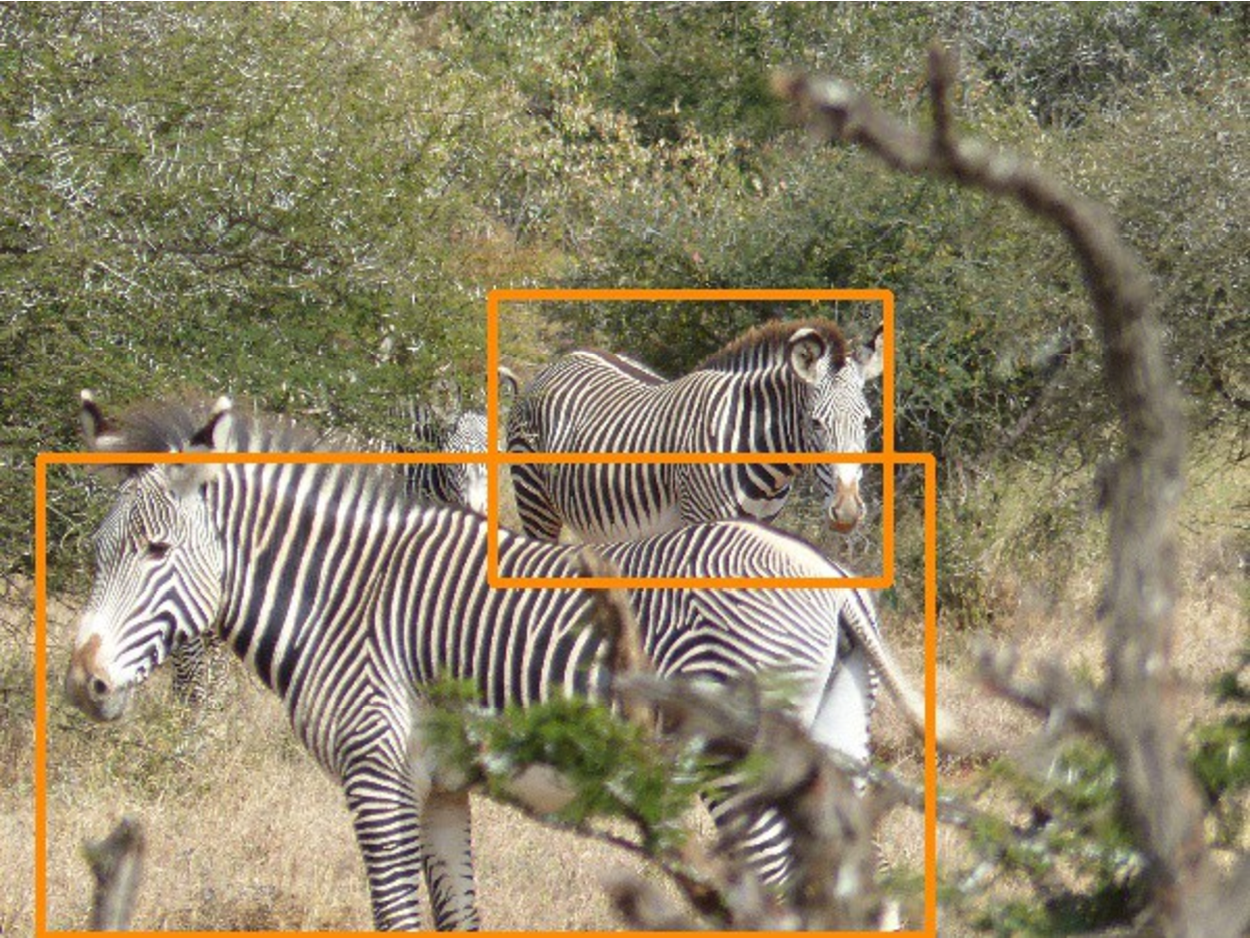
\includegraphics[width=0.13\textwidth]{resources/detections-rcnn-gz4.pdf} &
            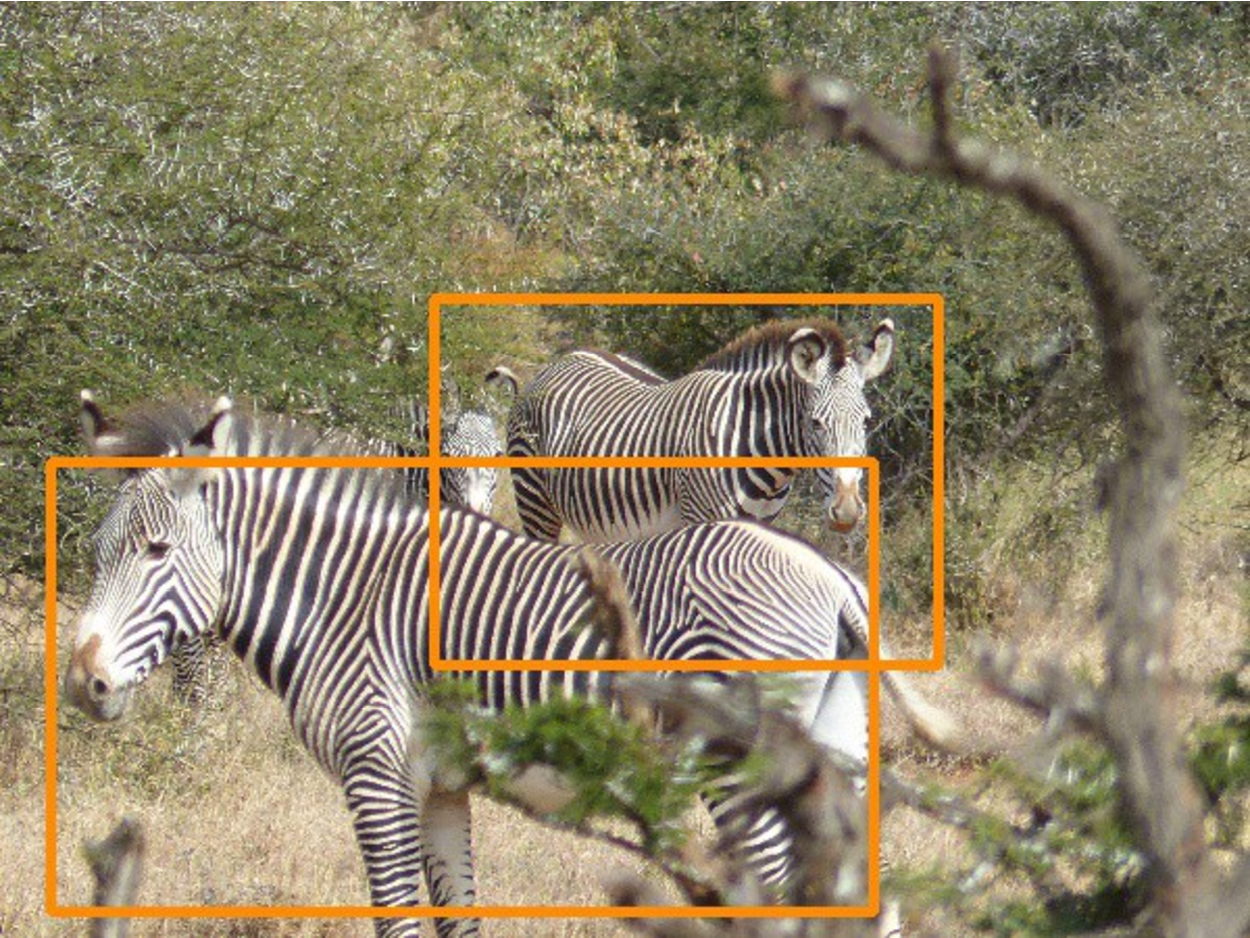
\includegraphics[width=0.13\textwidth]{resources/detections-yolo-gz4.pdf}   \\

            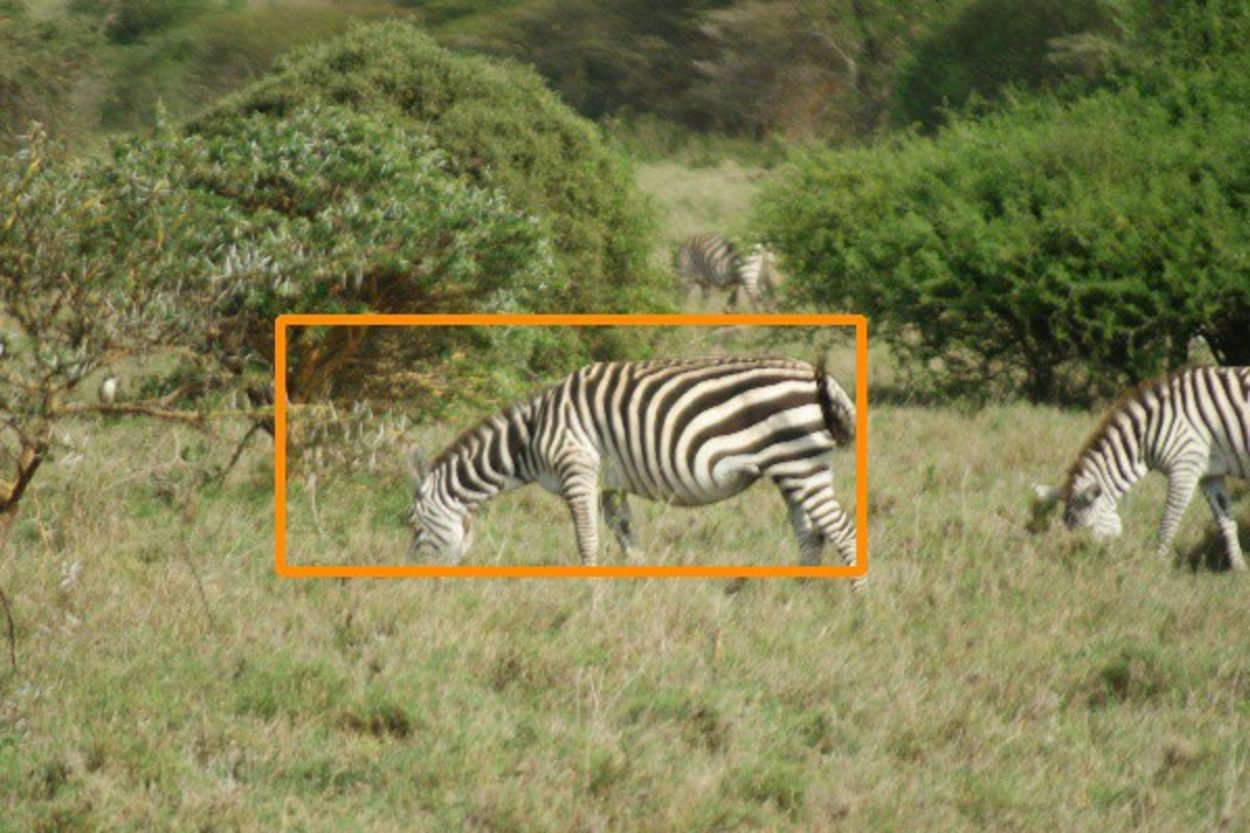
\includegraphics[width=0.13\textwidth]{resources/detections-rf-pz1.pdf}   &
            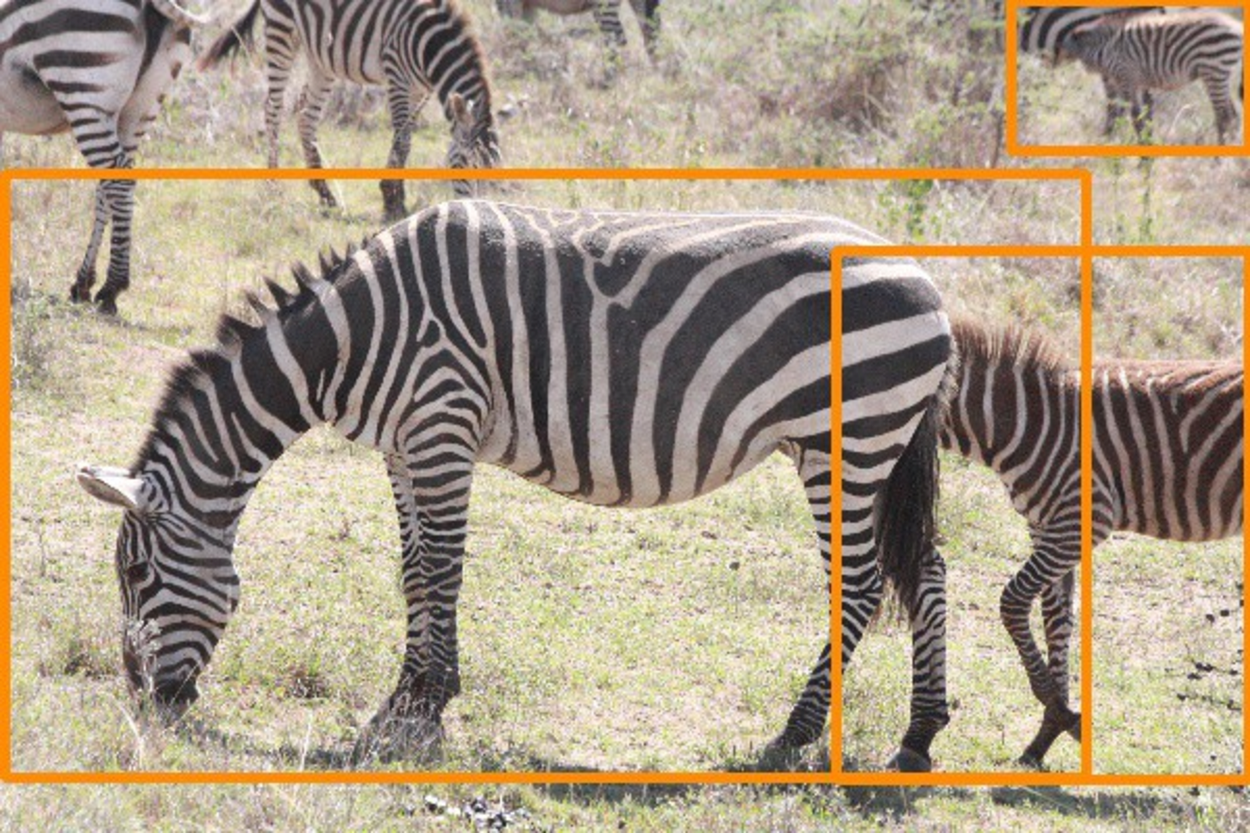
\includegraphics[width=0.13\textwidth]{resources/detections-rcnn-pz5.pdf} &
            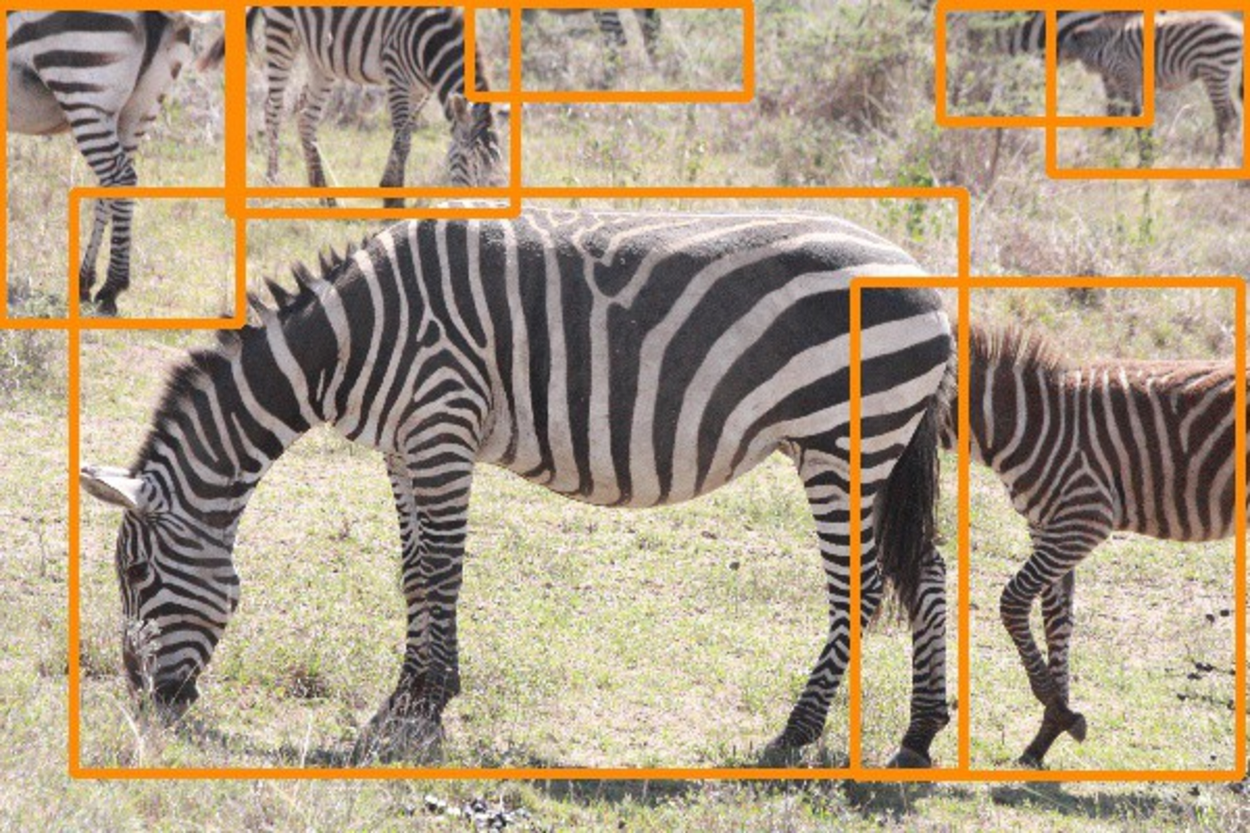
\includegraphics[width=0.13\textwidth]{resources/detections-yolo-pz5.pdf} &
            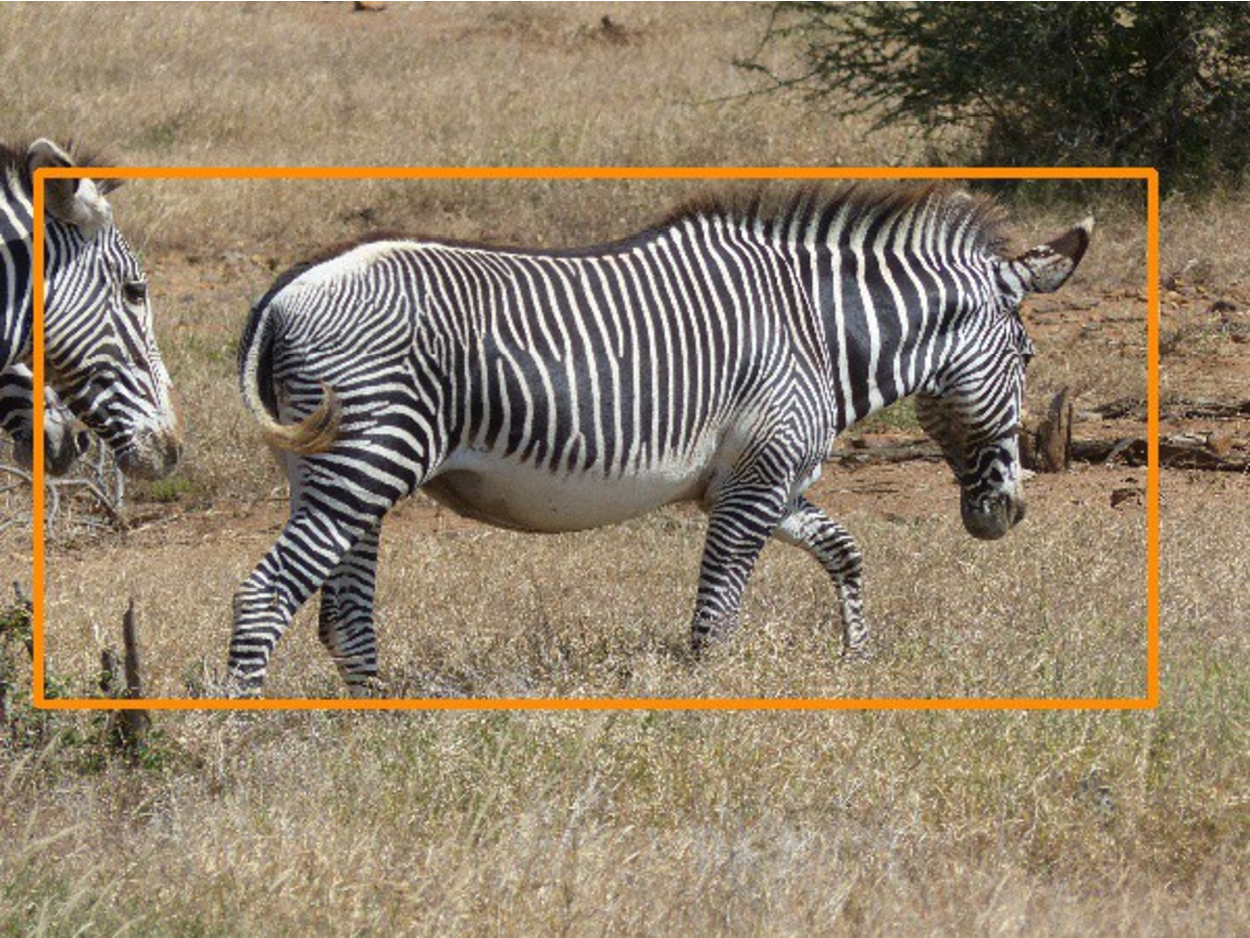
\includegraphics[width=0.13\textwidth]{resources/detections-rf-gz5.pdf}   &
            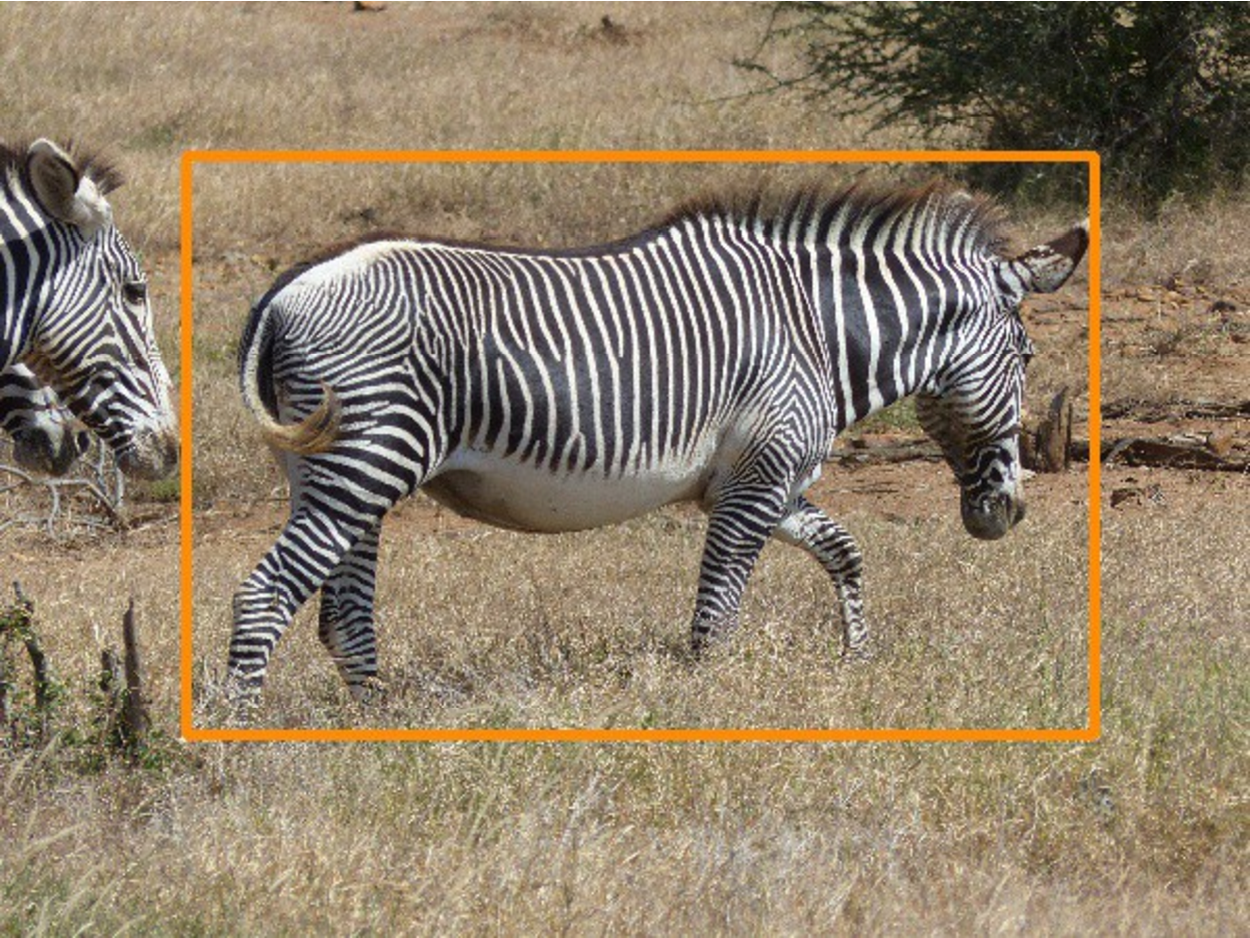
\includegraphics[width=0.13\textwidth]{resources/detections-rcnn-gz5.pdf} &
            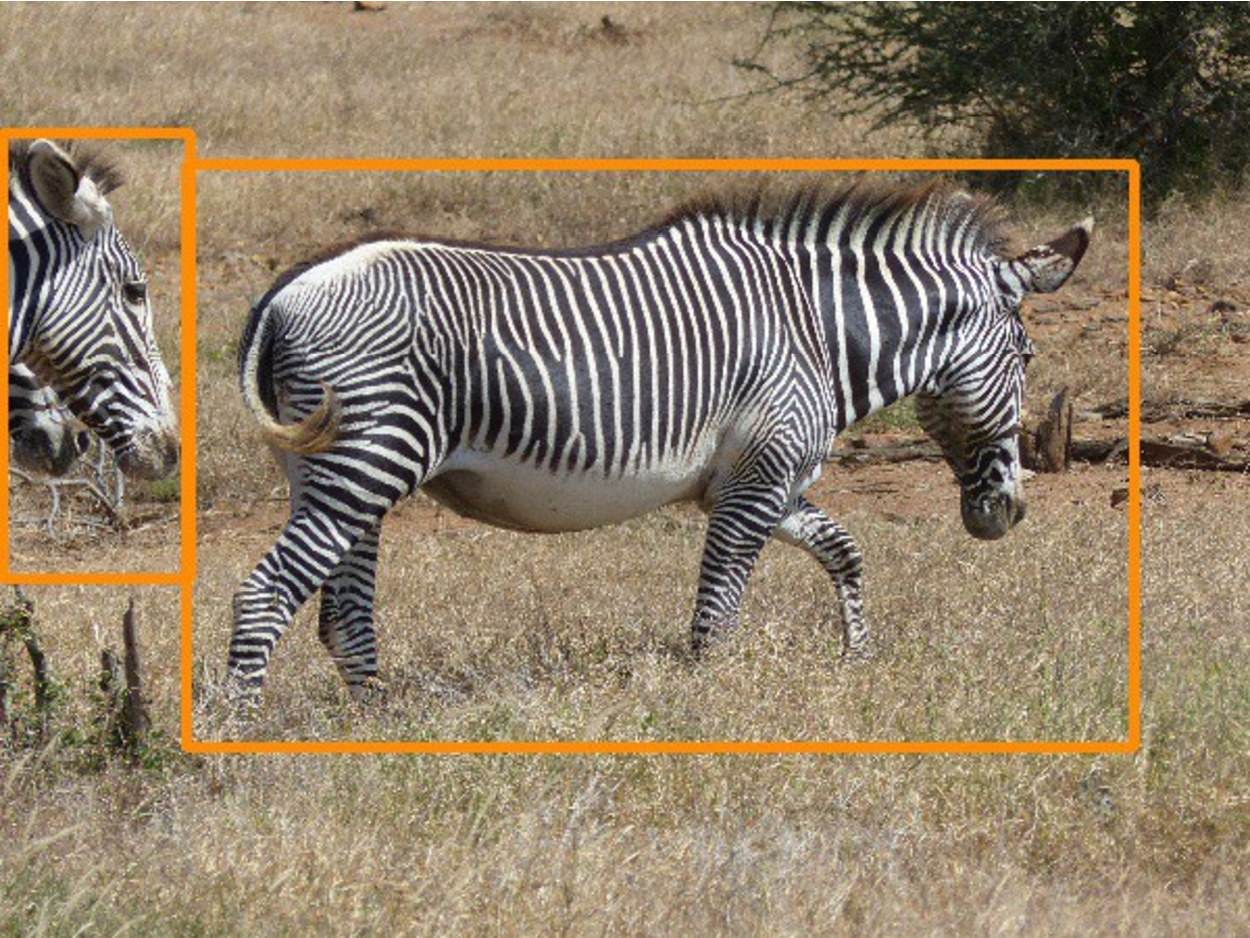
\includegraphics[width=0.13\textwidth]{resources/detections-yolo-gz5.pdf}   \\

            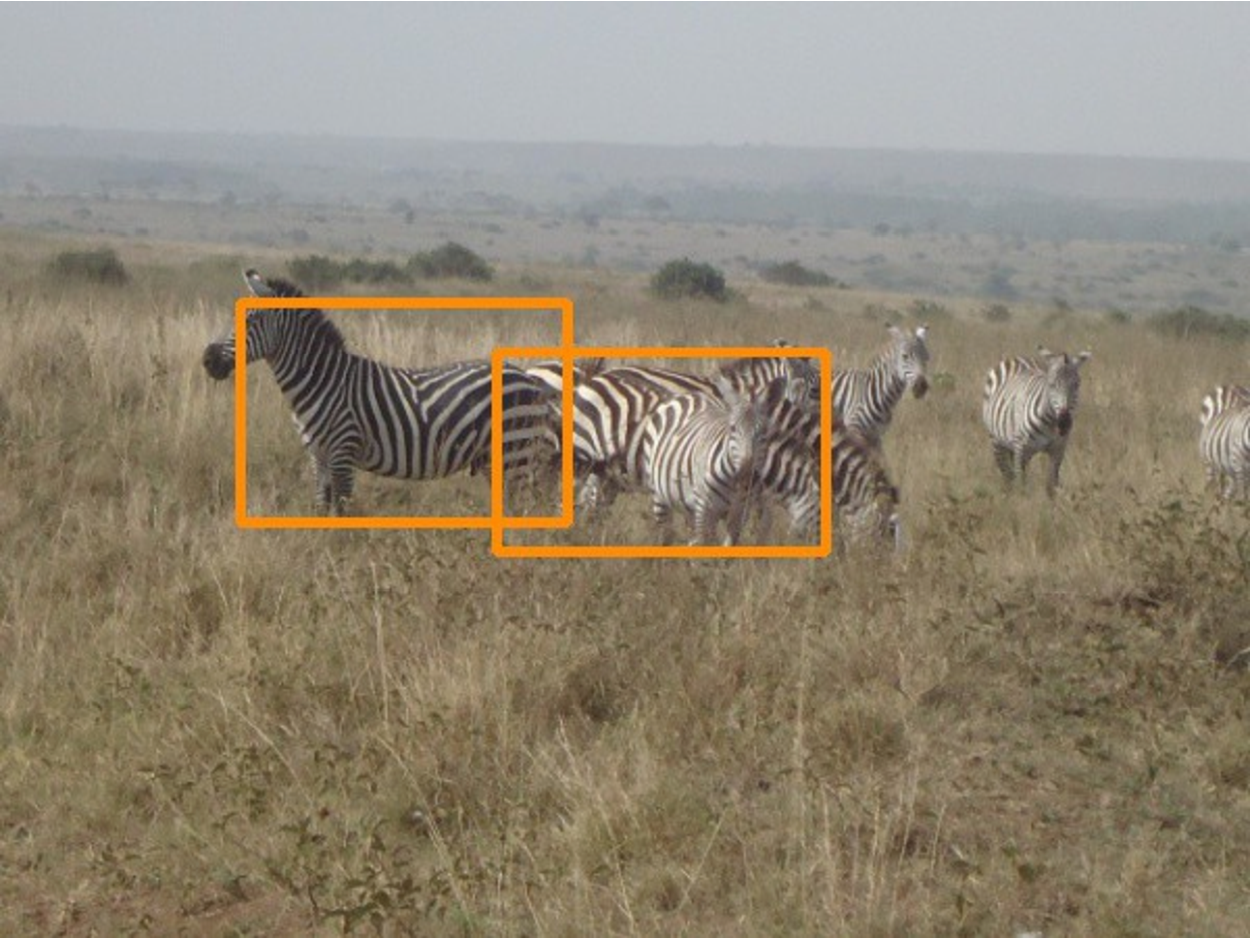
\includegraphics[width=0.13\textwidth]{resources/detections-rf-pz6.pdf}   &
            \includegraphics[width=0.13\textwidth]{resources/detections-rcnn-pz6.pdf} &
            \includegraphics[width=0.13\textwidth]{resources/detections-yolo-pz6.pdf} &
            \includegraphics[width=0.13\textwidth]{resources/detections-rf-gz6.pdf}   &
            \includegraphics[width=0.13\textwidth]{resources/detections-rcnn-gz6.pdf} &
            \includegraphics[width=0.13\textwidth]{resources/detections-yolo-gz6.pdf}   \\

            \includegraphics[width=0.13\textwidth]{resources/detections-rf-pz7.pdf}   &
            \includegraphics[width=0.13\textwidth]{resources/detections-rcnn-pz7.pdf} &
            \includegraphics[width=0.13\textwidth]{resources/detections-yolo-pz7.pdf} &
            \includegraphics[width=0.13\textwidth]{resources/detections-rf-gz7.pdf}   &
            \includegraphics[width=0.13\textwidth]{resources/detections-rcnn-gz7.pdf} &
            \includegraphics[width=0.13\textwidth]{resources/detections-yolo-gz7.pdf}   \\

            \includegraphics[width=0.13\textwidth]{resources/detections-rf-pz8.pdf}   &
            \includegraphics[width=0.13\textwidth]{resources/detections-rcnn-pz8.pdf} &
            \includegraphics[width=0.13\textwidth]{resources/detections-yolo-pz8.pdf} &
            \includegraphics[width=0.13\textwidth]{resources/detections-rf-gz8.pdf}   &
            \includegraphics[width=0.13\textwidth]{resources/detections-rcnn-gz8.pdf} &
            \includegraphics[width=0.13\textwidth]{resources/detections-yolo-gz8.pdf}   \\

            \includegraphics[width=0.13\textwidth]{resources/detections-rf-pz9.pdf}   &
            \includegraphics[width=0.13\textwidth]{resources/detections-rcnn-pz9.pdf} &
            \includegraphics[width=0.13\textwidth]{resources/detections-yolo-pz9.pdf} &
            \includegraphics[width=0.13\textwidth]{resources/detections-rf-gz9.pdf}   &
            \includegraphics[width=0.13\textwidth]{resources/detections-rcnn-gz9.pdf} &
            \includegraphics[width=0.13\textwidth]{resources/detections-yolo-gz9.pdf}   \\

            HF PZ                                                                     &
            R-CNN PZ                                                                  &
            YOLO PZ                                                                   &
            HF GZ                                                                     &
            R-CNN GZ                                                                  &
            YOLO GZ
        \end{tabular}
        \caption{Example images of detections on a set of 20 images for plains zebra (PZ) and Gr\'evy's zebra (GZ).  The operating point was set to 0.8 for the CNNs and 0.6 for Hough Forests (HF).  \copyright 2016 IEEE. Reprinted, with permission, from: J. Parham and C. Stewart, ``Detecting plains and Grevy’s zebras in the real world,'' in \textit{IEEE Winter Conf. Applicat. Comput. Vis. Workshops}, Lake Placid, NY, USA, Mar. 2016, pp. 1–9.}
        \label{fig:detections}
    \end{center}
\end{figure}

The three detectors were evaluated by calculating the IOU (intersection over union) percentage between the detections and the ground-truth.  A detection was considered correct if 1) the bounding box \text{IOU} $\geq$ 0.5 and 2) the species classification was correct.  A classification error is when the IOU threshold was satisfied for a predicted bounding box but had an incorrect species label.  Otherwise, the annotation was marked as having a localization error (not detected at all).  Looking at Table~\ref{tab:errors} showing detection performance on the DETECT dataset, we can see that Hough Forests makes by far the most classification and location errors.  The combined YOLO network achieves the highest number of correct detections overall but makes the most classification errors compared to the other two algorithms; Faster R-CNN makes more localization errors but rarely makes an incorrect classification.  Hough Forests makes the fewest classification errors, but this can be deceiving since it has almost double the number of localization errors as YOLO.  Side-by-side example detections for all of the algorithms can be seen in Figure~\ref{fig:detections}.  Overall, the YOLO V2 detector has the highest number of correct detections (56.0\%) compared to Faster R-CNN (51.7\%) and Hough Forests (40.2\%) on the DETECT dataset, on top of being the fastest. Therefore, YOLO V2 is selected for all further analyses of detection performance.

\begin{figure}[!t]
    \begin{center}
        \includegraphics[width=0.48\linewidth]{resources/localizer-pr-all-a.pdf}
        \hspace{1mm}
        \includegraphics[width=0.48\linewidth]{resources/localizer-pr-all-b.pdf}
    \end{center}
    \caption{The annotation localizer precision-recall curves (left) reports an unfiltered mean average-precision (mAP) of 81.7\% across all six species with an Intersection-over-Union (IoU) threshold of 50\%.  The drastic drop in performance of the plains zebra species can be contributed to the high number of background  -- likely small-sized -- annotations for this species; focusing on just AoIs (right) increases mAP to 90.6\%.  \copyright 2018 IEEE. Reprinted, with permission, from: J. Parham \textit{et al.}, ``An animal detection pipeline for identification,'' in \textit{IEEE Winter Conf. Applicat. Comput. Vis.}, Lake Tahoe, CA, USA, Mar. 2018, pp. 1–9.}
    \label{fig:performance-localizer}
\end{figure}

The YOLO localization model has different performance curves for each species in WILD.  The YOLO detector achieves a detection Average Precision (AP) of 57.6\% for plains and 76.2\% for Gr\'evy's, as calculated by the area under a Precision-Recall curve.  The whale fluke and sea turtle localizations achieve an AP of 99.0\% and 93.5\%, respectively.  This high level of performance makes intuitive sense because a mostly rigid animal sighted against a stark background of the sea, ocean floor, or sky will be easier to localize than a compact herd of overlapping, occluded animals.  As displayed in Figure~\ref{fig:performance-localizer} (left), the difference in difficulty can be seen noticeably in the relatively poor performance of the plains zebra localizations at only 57.5\%.  By referencing Table~\ref{table:dataset} we can see that the ratio of easy-to-find annotations (Annotations of Interest) to all annotations is the lowest at 19.2\% for plains zebras compared to the average of 42.2\% for all species.  Furthermore, the ratio of annotations per image for plains zebra is the highest at 2.9 compared to the average of 1.6.  Nevertheless, the YOLO localizer achieves an mAP of 81.7\% across all species, suitable for generalized detection.

The performance of the localizer is further analyzed when only annotations marked as AoIs are considered, see Figure~\ref{fig:performance-localizer} (right).  AoIs should be distinguishable, relatively large, and free of significant occlusions (a formal definition of AoI is provided later in Section~\ref{sec:aoi}).  The annotation localization performance drastically improves the detection Recall for all species when only AoIs are considered, with the most improvement being achieved by the plains zebra localizations.  This improvement indicates that most of the localization errors -- across the board for all species -- are from the background, small, occluded, or otherwise unidentifiable animals.  Missing these detections is less of a concern because we do not care to process them with ID.  By adjusting the goal of the localizer to focus on maximizing performance for AoIs, the YOLO model can achieve an mAP of 90.6\% on the WILD dataset, a significant improvement.

In summary, the creation of annotations by the localizer sets the context for which areas of an image are likely identifiable.  Furthermore, the goal of an identification process is to match \textit{comparable} sightings of animals; one of the most primitive pieces of information for determining if two annotations are comparable is their species. For example, it would not make sense to try and compare a zebra to a giraffe because the match will always have a predictable (negative) result. However, as discussed next, knowing the species is not the only kind of ecological metadata helpful in determining if two annotations are comparable.

\section{Annotation Labeling} \label{sec:labeler}

The third component of the detection pipeline is designed to re-classify the annotations produced by the previous localization stage.  The primary purpose of the annotation classification network (also known as the ``annotation labeler'') is flexibility.  For example, the species-only classification output of the localizer may not be the final (or only) intended metadata for an annotation.  Furthermore, it may be impractical to retrain the entire localizer when a new classification need comes up.  A practical use case of the labeler is that it allows the pipeline to predict a species \textit{and} a viewpoint for annotations.  This function is handy for identification because knowing the viewpoint of an animal allows for incompatible annotations to be filtered out, even more so than compared to only filtering on species.  It also allows for the localization network to be trained at a different level of abstraction when considering the ground-truth labels.  For example, we may train the localizer to focus on a general ``zebra'' class (e.g., to optimize localization performance) but use the labeler to re-classify annotations as ``Gr\'evy's zebra'' or ''plains zebra'', and add viewpoint classification support.

The labeler network uses smaller 128$\times$128-pixel images as input; the annotation bounding boxes from the localization network are cropped out of the original image and are re-sized to the correct input dimensions.  Input images are reduced to a 5$\times$5$\times$256 convolutional feature vector for classification via convolutional, max pooling, and batch normalization~\cite{ioffe_batch_2015} (BN) layers.  The network then adds a 512-dimension dense layer, followed by a feature pooling layer, a Dropout layer ($p=0.5$), and another 512-dimension dense classification layer.  The species and viewpoints are combined into paired classifications for the last dense layer of the network (activated by softmax), and the model's weights are optimized using the standard categorical cross-entropy loss.

The annotation labeler's architecture is similar to the WIC component, except it performs a standard single-prediction, multi-target classification. In addition, a separate set of weights (also initialized with transfer learning) is intentionally trained for the convolutional feature extractors in the WIC and labeler detection pipeline components.  This separation increases redundancy but also allows for specialized filters to be learned for each task; each detection component can be independently optimized without needing to re-validate the performance impact of a unified feature extraction across the entire pipeline.  Another reason the convolutional filters are not shared across components is that the input image sizes are fundamentally very different since they are trying to capture different levels of detail.  For example, the WIC is tasked with animal existence at an image level. In contrast, the labeler is sometimes tasked with differentiating similar species and viewpoints at an annotation level.

\subsection{Results}

\begin{figure}[!t]
    \begin{center}
        \includegraphics[width=0.93\linewidth]{resources/labeler-roc.pdf}
    \end{center}
    \caption{The ROC performance curves for the annotation classifier (labeler) suggests that the component is very accurate at predicting the species of an annotation.  \copyright 2018 IEEE. Reprinted, with permission, from: J. Parham \textit{et al.}, ``An animal detection pipeline for identification,'' in \textit{IEEE Winter Conf. Applicat. Comput. Vis.}, Lake Tahoe, CA, USA, Mar. 2018, pp. 1–9.}
    \label{fig:labeler-roc}
\end{figure}

The annotations are labeled with a viewpoint of the animal relative to the camera.  The viewpoints for zebras and giraffes in the WILD dataset are labeled with one of 8 discretized yaw locations around the animal, from the set \{\texttt{front}, \texttt{front-right}, \texttt{right}, \texttt{back-right}, \texttt{back}, \texttt{back-left}, \texttt{left}, \texttt{front-left}\}.  Sea turtles are commonly captured from above and sometimes from below, so their allowed viewpoints are constrained to the set of six viewpoints \{\texttt{front}, \texttt{right}, \texttt{back}, \texttt{left}, \texttt{top}, \texttt{bottom}\}.  Whale flukes also have a similar restriction where they are label from a set of 4 \{\texttt{top}, \texttt{bottom}, \texttt{right}, \texttt{left}\}, with the most common being \texttt{bottom} when the angled fluke is viewed above water.  The species and viewpoints pairs are combined into 42 distinct combinations (in the form \texttt{species:viewpoint}) to create the set of available classification labels for training.  The label pairing used by the annotation classifier does cause an inherent class imbalance, but achieving balanced viewpoints across all species in a real-world, unstructured setting is an impractical goal.  The real-world implication is that balanced training data for all categories is seldom possible when viewpoints are considered. Hence, the labeler needs to have some mechanism to counteract its effect on training.  The labeler addresses this problem by identifying the species and viewpoint combination with the fewest examples and sets a maximum number of examples for all categories in a given epoch as a fixed multiplier of that minimum (the experiments here set the multiplier to 4).

\begin{figure}[!t]
    \begin{center}
        \includegraphics[width=0.92\linewidth]{resources/labeler-confusion.pdf}
    \end{center}
    \caption{The classification confusion matrix for the annotation classifier (labeler), marked with abbreviated \{\texttt{species:viewpoint}\}.  The species abbreviations are: \texttt{MG} for Masai giraffe, \texttt{RG} for reticulated giraffe, \texttt{ST} for sea turtle, \texttt{WF} for whale fluke, \texttt{GZ} for Gr\'evy's zebra, and \texttt{PZ} for plains zebra.  The viewpoint abbreviations are: \texttt{left} (L), \texttt{front-left} (FL), \texttt{front} (F), \texttt{front-right} (FR), \texttt{right} (R), \texttt{back-right} (BR), \texttt{back} (B), and \texttt{back-left} (BL).  The white boxes represent the separate species classes where values outside of these boxes indicate incorrect species predictions.  The classifier predicted the correct species and viewpoint for 61.7\% of the examples and the correct species for 94.3\% of the examples.  \copyright 2018 IEEE. Reprinted, with permission, from: J. Parham \textit{et al.}, ``An animal detection pipeline for identification,'' in \textit{IEEE Winter Conf. Applicat. Comput. Vis.}, Lake Tahoe, CA, USA, Mar. 2018, pp. 1–9.}
    \label{fig:labeler-confusion}
\end{figure}

As seen in Figure~\ref{fig:labeler-roc}, the species-specific ROC curves achieve at least 96.7\% AUC across all species in the WILD dataset.  The species ROC operating curves in this figure are calculated by taking an average over the associated ROC curves for its respective viewpoints.  Furthermore, the effect of species and viewpoint classification can be visualized in Figure~\ref{fig:labeler-confusion}.  The overall accuracy of species and viewpoint combination classifications is 61.7\% over 42 distinct categories for species and viewpoints combined.  The accuracy improves from this baseline when we consider how slight changes in viewpoint impacts identification (i.e., a $\pm$ 45\% degree shift in yaw is tolerable~\cite{crall_hotspotter_2013} for giraffes and zebras), which achieves an 87.1\% ``fuzzy'' accuracy.  The white squares in Figure~\ref{fig:labeler-confusion} indicate different species, and any values in the matrix outside of the squares represent incorrect species classifications.  If we examine the errors outside the white boxes, then the inter-species classification accuracy is 94.3\%.  We can see that the majority of the inter-species classification error is between the two sub-genus species of giraffes (37.4\% of the species classification errors) and some extra error between the two zebra classes (25.2\%).  These failures make intuitive sense as the species look relatively similar and can have subtle differences between their appearances at oblique viewpoints.  It is worth noting here that the whale fluke and sea turtle species have almost no inter-species confusion, supported by their ROC AUC values of 99.8\% and 98.3\%, respectively.  Of the species errors made, 62.9\% are due to incorrect sub-genus giraffe and zebra classifications.  In summary, the overall genus (zebras vs.\ giraffes vs.\ whale flukes vs.\ sea turtles) classification accuracy is 97.9\%.

Now that we have bounding boxes with species and viewpoint labels, we need to consider how well the boxes represent the animals they surround.  The use of axis-aligned bounding boxes is a good tool for finding animals but can be an inefficient structure when used to represent animals that are not rectangular.  For example, giraffes have long legs and necks, and a rectangular bounding box around an animal can include considerable amounts of distracting background information.  The next component is designed to address this problem by roughly distinguishing an animal from its surroundings.

\section{Coarse Background Segmentation} \label{sec:background}

\begin{figure}[!t]
    \begin{center}
        \includegraphics[width=0.32\linewidth]{resources/background-input.pdf}
        \includegraphics[width=0.32\linewidth]{resources/background-weights.pdf}
        \includegraphics[width=0.32\linewidth]{resources/background-sift.pdf}
    \end{center}
    \caption{The locations of SIFT keypoints are not semantically constrained to the animal body and, if added to an identification search database, can confuse the ranking algorithm and exacerbate known issues like scenery matching.  The coarse background segmentation model allows for SIFT keypoints to be down-weighted based on how much they contain background information.  Yellow keypoints have a higher weight compared to blue keypoints.}
    \label{fig:weighting}
\end{figure}

The fourth detection pipeline component attempts to produce a coarse segmentation of an animal.  The modifier ``coarse'' is intentionally added to the method description because it is not meant to be (or compete with) a pixel-level semantic segmentation algorithm~\cite{uijlings_selective_2013,girshick_rich_2014,ronneberger_u-net:_2015,leibe_robust_2008,van_de_sande_segmentation_2011}.  Instead, a classification technique is presented that \textit{approximates} a pixel-level segmentation by creating a binary classification map.  The task is to take an annotation (with a species provided by the labeler) and roughly classify which pixels belong to that species versus the background.  The goal is to generate a rough background mask that can eliminate or otherwise down-weight distracting non-animal pixel information.  For example, the output of this component can be used to calculate weights for SIFT~\cite{lowe_distinctive_2004} keypoints and the features used by an identification pipeline.  An example of this type of keypoint weighting can be seen in Figure~\ref{fig:weighting} with the HotSpotter algorithm~\cite{crall_hotspotter_2013}.  Key design features of this component are: 1) it only requires species-labeled bounding boxes for ground-truth and does not require fully-segmented images, 2) it is trained on small positive or negative patches as a binary classifier, and 3) it is applied fully convolutionally across an entire input image to produce a rough semantic segmentation map.

The annotation background segmentation approach uses a distinct type of neural network architecture called a Fully Convolutional Neural Network (FCNN)~\cite{long_fully_2015}.  An FCNN is a special kind of CNN with no dense (fully-connected) layers and supports arbitrarily large input image sizes.  This input size flexibility requires that the network be composed entirely of convolutions, pooling layers, or other non-rigid layers.  This design feature is exploited by training the network on a fixed input size and performing forward inference on an arbitrarily large image (that must be equal to or larger than the training size).  During training, 48$\times$48-pixel input patches are reduced via convolutional and max-pooling layers to a 1$\times$1-pixel patch with 128 channels (a spatial size of one pixel).  It is then classified with a dropout layer($p=0.4$) and a (1$\times$1 Network-in-Network~\cite{lin_network_2013} convolutional layer with two outputs (binary classification).  During inference, the network's output is expected to increase to W$\times$H$\times$128, where $W$ and $H$ are down-sampled resolutions of the original input size (at least 48 pixels), and the classification output is run to produce a binary classification map of size W$\times$H$\times$2.  An FCNN can be efficiently applied across an entire image, without the need to resort to computationally intensive methods like sliding windows~\cite{krizhevsky_imagenet_2012}, shift-and-stitch~\cite{sermanet_overfeat:_2013}, or memoization~\cite{esmaeilzadeh_neural_2012,graham_spatially-sparse_2014,zlateski_znnfast_2016}.  Importantly, the last layer's softmax activation is applied along the channel dimension, which means it can dynamically expand to the spatial output of a test image to create an automatic classification map.

\begin{figure}[!t]
    \begin{center}
        \includegraphics[width=0.7\linewidth]{resources/patches.pdf}
    \end{center}
    \caption{An illustration of the background segmentation patch sampling (using giraffes) and the utility of a cleaning procedure.  The target giraffe (green, solid) has a collection of labeled positive patches (blue and red) and negative patches (orange) that are sampled outside the bounding box.  The blue patches are \textit{true} positives whereas the red patches are incorrectly-labeled \textit{true} negatives.  The goal of the cleaning procedure is to convert all red boxes into orange boxes automatically.  Best viewed in color.  \copyright 2018 IEEE. Reprinted, with permission, from: J. Parham \textit{et al.}, ``An animal detection pipeline for identification,'' in \textit{IEEE Winter Conf. Applicat. Comput. Vis.}, Lake Tahoe, CA, USA, Mar. 2018, pp. 1–9.}
    \label{fig:patches}
\end{figure}

\subsection{Patch-based Training}

The patch training data is generated by selecting a target annotation and resampling its image such that the bounding box has a fixed width of 300 pixels.  Then, random patch locations are sampled uniformly across the image (and for a range of scales) where positive patches are centered inside the annotation (or an annotation of the same species), and negative patches are centered outside all annotations for that species.  Positive patch exemplars are therefore species-specific and are meant to cover sub-regions within an animal body. In contrast, negative patches represent background foliage, terrain, and other animals of different species.

The proposed positive patch sampling scheme can be problematic, however.  The bounding box localizations of giraffes, for example, generally have large amounts of negative space around the neck and the legs (see Figure~\ref{fig:patches}).  When positive patches are sampled from inside giraffe bounding boxes, some are incorrectly labeled as positive that contain only negative background pixel information (red boxes).  A self-supervised cleaning procedure is used during training to help correct label noise in the dataset.  At the start of training, the network is given the original labels and asked to perform binary classification on the data as-is.  Each time the learning rate decreases (and only after the model achieves an overall accuracy $\geq$ 90\%), the currently learned model is run on the training and validation data to find any incorrect labels.  Any label with a $\geq$ 95\% prediction of belonging to the opposite ground-truth label is automatically ``cleaned'' and its binary label flipped.  The cleaning procedure has been found to help smooth out training and drastically improve the final results' qualitative performance.

\subsection{Results with Fully-Convolutional Inference}

\begin{figure}[!t]
    \begin{center}
        \includegraphics[width=0.78\linewidth]{resources/samples-image-giraffe_masai.pdf} \\
        \vspace{0.040cm}
        \includegraphics[width=0.78\linewidth]{resources/samples-image-giraffe_masai2.pdf} \\
        \vspace{0.040cm}
        \includegraphics[width=0.78\linewidth]{resources/samples-image-giraffe_reticulated.pdf} \\
        \vspace{0.040cm}
        \includegraphics[width=0.78\linewidth]{resources/samples-image-giraffe_reticulated2.pdf} \\
        \vspace{0.040cm}
        \includegraphics[width=0.78\linewidth]{resources/samples-image-turtle_sea.pdf} \\
        \vspace{0.040cm}
        \includegraphics[width=0.78\linewidth]{resources/samples-image-turtle_sea2.pdf} \\
        \vspace{-0.040cm}
        \includegraphics[width=0.78\linewidth]{resources/samples-image-whale_fluke.pdf} \\
        \vspace{-0.040cm}
        \includegraphics[width=0.78\linewidth]{resources/samples-image-whale_fluke2.pdf} \\
        \vspace{-0.040cm}
        \includegraphics[width=0.78\linewidth]{resources/samples-image-zebra_grevys.pdf} \\
        \vspace{0.040cm}
        \includegraphics[width=0.78\linewidth]{resources/samples-image-zebra_grevys2.pdf} \\
        \vspace{0.040cm}
        \includegraphics[width=0.78\linewidth]{resources/samples-image-zebra_plains.pdf} \\
        \vspace{0.040cm}
        \includegraphics[width=0.78\linewidth]{resources/samples-image-zebra_plains2.pdf}
    \end{center}
    \caption{A grid of background classifications for six species shows that the component is able to learn useful background subtraction masks.  These masks function as semantic segmentations between the species of interest and the background and do not distinguish animal instances.  \copyright 2018 IEEE. Reprinted, with permission, from: J. Parham \textit{et al.}, ``An animal detection pipeline for identification,'' in \textit{IEEE Winter Conf. Applicat. Comput. Vis.}, Lake Tahoe, CA, USA, Mar. 2018, pp. 1–9.}
    \label{fig:background}
\end{figure}

Since the annotation background network was trained on noisy, patch-based data -- and with the lack of fully-segmented ground-truth in WILD -- a quantitative segmentation metric for the model's performance cannot be provided.  However, looking at Figure~\ref{fig:background}, the background segmentation network performs well on various annotations of a known species to classify regions of the image as background and foreground.  In this figure, the binary output masks of the background classification network are combined with their associated input annotations.  Something to note is that the lack of distinction between class instances and animals with the same species in the annotation will not be masked out.  Work by Crall (see Section 3.5.4 in ~\cite{crall_identifying_2017}) shows the positive impact of using the coarse background segmentation; overall, identification matching accuracy improves when a background mask is used for feature weighting.  The experiment presented in that work shows top-1 ranking improvements for Gr\'evy's and plains zebra of approximately 5\% for comprehensive ID experiments.

The creation of segmentation maps helps reduce the distracting background information within an annotation. However, we have not addressed the problem of knowing which annotations are producing distracting \textit{foreground} information.  For example, an annotation may show an occluded, blurry, or truncated (cut in half by a tree) animal and should ideally not be provided to ID. Therefore, the next pipeline stage takes a step back and determines which annotations in an image were likely captured by accident.  The general assumption is that incidental background sightings most likely have less useful visual information for ID and should be filtered out proactively.

\section{Annotation of Interest (AoI)} \label{sec:aoi}

The fifth and final detection component focuses on determining which animal annotations in an image are good candidates for identification.  The goal of AoI classification is to try and answer the question, ``\textit{why did the photographer take this picture?}'' and is tasked with distinguishing the animals that were the intended subject(s) (i.e., the ``Annotations of Interest'') from incidental background sightings of animals.  It is important to note that this task tries to understand the composition of an image \textit{a posteriori} to help guide ID and is not concerned with the aesthetic form of a particular image or calculated focus points.  Instead, the Annotation of Interest (AoI) classifier identifies the most prominent animals in the image because they are likely to be the most identifiable.  While state-of-the-art object detection algorithms are often compared and evaluated on their ability to localize \textit{all} objects of interest captured in an image -- regardless of the pose, lighting, aspect ratio, focus, scale, level of obscurity, or degree of truncation -- a different objective is needed when animal ID is the intended use case: one that can be optimized for only detecting \textit{identifiable} animals.  To do this, though, we first need to know which annotations are even identifiable because the value of an animal detection should be fundamentally tied to the amount of identifying visual information it provides.

\begin{figure}[!t]
    \begin{center}
        \includegraphics[width=0.90\linewidth]{resources/overview.pdf}
    \end{center}
    \caption{An example image captured by a citizen scientist during an animal photographic census.  We may ask, ``\textit{which animal was the intended subject of this image (if any)?}''  The animal with a green box around it is the Annotation of Interest for this image and all other animals should be considered incidental background sightings.}
    \label{fig:overview}
\end{figure}

Figure~\ref{fig:overview} shows a motivating example for why the concept of AoI is needed. There are 22 plains zebras in this picture, presenting five different viewpoints and varying degrees of truncated and obscured animals.  The classic formulation of object detection would expect 22 bounding boxes as the optimal output.  In terms of identifiability, it is clear that the green highlighted box offers the best visual information out of all of the animals that are seen.  The animal is well lit, in focus, not obscured or truncated, captured at a good resolution, and was perhaps the primary subject of the image when the photographer took the image.  The dark blue box arguably ranks as the second-best zebra annotation but is slightly out of focus and is half-occluded.  Did the photographer intend to photograph the blue animal, or was it simply in the background?  Perhaps either way.  The red box (upper right corner), in contrast, is an animal that is significantly obscured by grass and is most certainly an accidental capture because it offers almost no usable information for ID.  While the red box may be a challenging detection to predict correctly (i.e., an understandable failure), we can expect that the light blue box to be within the capabilities of a modern, deep learning-based object detector to find correctly (and predict a species and viewpoint label as a left-side plains zebra).  The problem is that the light blue box could be considered a legitimate detection even though it offers little identifying information and is only slightly more valuable to ID than the red box.  As such, the green box was most likely the intended subject considering the scene's composition and should be regarded as an AoI.  Only the green box should be considered an AoI in this image, and all other animals are incidental sightings of animals in the background.  The critical insight with AoI is that the localizer can de-prioritize failures for background animals because they often do not contribute meaningful ID information.  To define the concept more formally, an AoI should have most or all of the following properties:

\squishlist
\item is of a distinguishable individual animal (i.e., free-standing, well-lit, clearly visible),
\item is relatively large and has decent resolution,
\item is commonly located near the center of the image, and
\item is in focus and not blurred
\squishend

\noindent Conversely, an annotation should not be considered an AoI if it has one or more of the following opposite properties:

\squishlist
\item is a part of an overlapping herd or group of animals
\item is relatively small or contains few pixels
\item is out of focus or is otherwise blurry
\item is located around the edges of the image
\item is occluded by other animals or objects by area $\geq$ 25\%
\item is off the edge of the frame of the image by area $\geq$ 25\%
\squishend

\noindent The properties of AoIs demand that an annotation not be reviewed in isolation (i.e., by only viewing its cropped sub-region).  The decision that an annotation is an AoI must be made by weighing the entire image context as well as against any other accompanying annotations.  This process is naturally subjective and can be hard to determine reliably for borderline cases.  Further, because these conditions are relatively strict, there are rarely more than one or two AoIs in a particular image, and some images with detected annotations have no AoIs.  In summary, the reason to use Annotations of Interest is motivated by its two primary use cases:

\numsquishlist
\item preventing partial-animal, background, and otherwise visually distracting detections from entering an automated animal identification pipeline, and
\item training citizen scientist volunteers on how best to take high-quality images for photographic censusing.
\numsquishend

\noindent Annotation of Interest was the first attempt at addressing the annotation filtering problem.  Subsequent analysis in Chapter~\ref{chapter:ca} describes, evaluates, and deploys a more thorough and successful approach to the annotation filtering problem for animal ID. Nevertheless, the following discussion is still helpful since AoI is an image-level determination for the subject of an image and still helps with accurately tuning the localizer for finding well-formed annotations.

\subsection{AoI Ground-Truth \& Labeling Variability}

\begin{table}[!t]
    \caption{The number of the ground-truth AoI decisions made by different teams of human reviewers.  The teams were given the same instructions but split by their respective domains of expertise.}
    \label{tab:progress}
    \begin{center}
        \begin{tabular}{| l | l | r |}
            \hline
            \textbf{Team} & \textbf{Group}  & \textbf{AoIs} \\
            \hline\hline
            1             & Ecologists      & 5,166         \\
            \hline
            2             & Data Engineers  & 6,829         \\
            \hline
            3             & Computer Vision & 5,729         \\
            \hline
            4             & Data Scientists & 6,174         \\
            \hline
            5             & Author          & 5,547         \\
            \hline
        \end{tabular}
    \end{center}
\end{table}

The decision to label an annotation an Annotation of Interest is inherently subjective.  It is, therefore, important that an image and all of its annotations be analyzed by multiple reviewers when ground-truth labels are being generated for training and evaluating AoI methods.  The ground-truth annotations in the WILD dataset were distributed to five different teams for labeling.  Each team had different background training and skillsets and -- even when provided with the exact same definition of an AoI and a handful of examples -- had different implicit reasonings and motivations for their decisions.  A brief description of each team is shown in Table~\ref{tab:progress} along with the total number of AoIs they marked (out of 9,871 considered annotations in the dataset).  The final ground-truth AoI labels for the annotations in WILD were created with a simple majority rule, requiring at least three out of the five teams to agree that an annotation needed to be considered an AoI.

The distribution of the labeling work was parallelized in two ways: across teams to increase redundancy and within teams to increase throughput.  The ``ecologist'' team was comprised of biologists and \textit{equid} experts, plus an array of undergraduate and graduate students, at Princeton University.  Working alongside the team of ecology researchers, a ``data engineering'' team comprised of data and software engineers based in Portland, OR also reviewed the same images to make independent AoI decisions.  The third ``computer vision'' team included computer vision and algorithm researchers at RPI, and the ``data scientist'' team was a group of data scientists and social network researchers at the University of Illinois, Chicago.  Each image in WILD was reviewed by at least one ecologist, one software engineer, one computer vision researcher, and one data scientist.  Lastly, the author of this dissertation worked alone (as the creator of the AoI concept) to independently label all of the annotations in the WILD dataset.  The variance between the various teams is relatively high, with the ecologist team deciding only 52.3\% of the annotations were AoIs compared to 69.2\% by the data engineer team. The average number of AoIs is 5,889$\pm$571 across all teams, representing 59.7\% of all detections in the dataset, but only 3,598 annotations (36.5\%) had a majority vote by at least three teams.

\begin{figure}[!t]
    \begin{center}
        \includegraphics[width=0.45\linewidth]{resources/centers-all-log2.pdf}
        \includegraphics[width=0.45\linewidth]{resources/centers-aoi-log2.pdf}
    \end{center}
    \caption{The distribution of bounding box center locations (on a unit square) for all annotations (left) and AoIs (right).  Annotations of Interest are much more uniform and biased towards the center.}
    \label{fig:ca-metrics-centers}
\end{figure}

\begin{figure}[!t]
    \begin{center}
        \vspace{1.0cm}
        \includegraphics[width=0.95\linewidth]{resources/areas.pdf}
    \end{center}
    \caption{A histogram of the total number of annotations and AoIs (y-axis) as a function of the percentage of the image area (x-axis, in 11 buckets each with a size of 10\%).  This shows that AoIs, compared to annotations in general, are much less likely to be small annotations.}
    \label{fig:ca-metrics-area}
\end{figure}

With ground-truth labels for AoI assigned to the dataset, we can analyze the unique qualities of AoIs and how they present themselves in images.  Figure~\ref{fig:ca-metrics-centers} plots the spatial distributions (on a normalized unit square) of AoI bounding boxes (right) as compared to all annotation bounding boxes (left) in the WILD dataset.  We can see that the centers of AoI bounding boxes seem to be biased towards the center of the image.  The area of AoI bounding boxes (shown in Figure~\ref{fig:ca-metrics-area}), as calculated by a percentage of the area of the whole image, also shows a clear inverse correlation with annotation size.  These results make intuitive sense because 1) an AoI is most likely going to be near the center of the image because it is strongly associated with finding the subject of an image and 2) any annotation that occupies under 20\% of the image area is most likely not an AoI because it is not sufficiently large to capture enough visual detail for the animal.

\subsection{Results}

\begin{figure}[!t]
    \begin{center}
        \includegraphics[width=0.75\linewidth]{resources/aoi-true.pdf} \\
        \vspace{0.040cm}
        \includegraphics[width=0.75\linewidth]{resources/aoi-false.pdf}
    \end{center}
    \caption{A positive AoI training example (top row) is comprised of the resampled RGB image (left) and the annotation segmentation mask (middle).  The right-most column depicts their combined representation.  As shown in the negative example (bottom row), the masked annotation is of an occluded, background animal and is not an AoI.  \copyright 2018 IEEE. Reprinted, with permission, from: J. Parham \textit{et al.}, ``An animal detection pipeline for identification,'' in \textit{IEEE Winter Conf. Applicat. Comput. Vis.}, Lake Tahoe, CA, USA, Mar. 2018, pp. 1–9.}
    \label{fig:aoi}
\end{figure}

The AoI classifier has a very similar convolutional and dense layer structure to the whole-image classifier (WIC) component, except for three differences: 1) it takes as input a 4-channel input image, comprised of red, blue, and green color channels stacked with a fourth annotation bounding box mask, 2) the output layer (with a softmax activation function) has only two outputs for simple binary classification, and 3) the network weights are optimized using categorical cross-entropy loss.  Examples of positive and negative training input images can be viewed in Figure~\ref{fig:aoi}.  The end goal of the AoI classifier is to eliminate the need to perform identification processing on the background and partially visible animals, and we will see in later chapters causes an increase in the total amount of work needed by human reviewers.

\begin{figure}[!t]
    \begin{center}
        \includegraphics[width=0.9\linewidth]{resources/aoi2-roc.pdf}
    \end{center}
    \caption{The ROC performance curves for the AoI classifier.  The species with the best AoI classification performance is plains zebra, mostly due to the lower AoI to annotations ratio.  The AoI classifier performs the worst on whale flukes and sea turtles because it is harder to tell when solitary animals should be considered AoIs.  \copyright 2018 IEEE. Reprinted, with permission, from: J. Parham \textit{et al.}, ``An animal detection pipeline for identification,'' in \textit{IEEE Winter Conf. Applicat. Comput. Vis.}, Lake Tahoe, CA, USA, Mar. 2018, pp. 1–9.}
    \label{fig:aoi2-roc}
\end{figure}

The AoI classifier achieves an overall accuracy of 72.8\% on the held-out test data (521 true positives, 1,268 true negatives, 506 false positives, 164 false negatives) when using a confidence threshold of 84\%.  Figure~\ref{fig:aoi2-roc} shows ROC curves for each species.  Ironically, the AoI classification performance of plains zebras shines, further supporting the claim that the background annotations for plains zebras in WILD are not good identification candidates.  However, we can see that the sea turtle and whale fluke AoI results are very close to random.  This poor performance is not surprising because those categories have the lowest percentage of AoIs relative to the number of annotations for that class, and the classifier struggles on solitary species with ambiguous AoI definitions.  The AoI classification is objectively the worst-performing component of the detection pipeline as it struggles with the overall ambiguity of the concept.  However, the primary goal of AoI selection is to reduce the overall number of poor annotations that are passed along to an identification pipeline.  From this point-of-view, the AoI classifier correctly eliminates from processing 71.5\% of background annotations at the cost of missing 23.9\% of the positive AoIs.  Furthermore, the ground-truth AoI data helps to better configure the localizer models during test time.

Let us now review the entire detection pipeline.  The detector pipeline produces a set of bounding box annotations from pre-filtered images.  Each of those annotations has a species and viewpoint label, a background mask, and an AoI classification, which can all be used to filter out irrelevant or distracting annotations or reduce distracting scenery.  Furthermore, the design of each of the above components puts few requirements on training data and can be bootstrapped quickly for new species using only bounding boxes.  While the specific components in this pipeline are not novel implementations -- and an in-depth analysis using alternative methods is not provided for most of the components -- that is not the core contribution. Instead, the point of the pipeline is to define a modularized structure for general animal detection, and its claim to novelty is in its comprehensive understanding of how animal detection is needed for real-world applications on animal ID.

\section{Additional Components \& Applications}

The core detection pipeline presented up till this point can be extended to work with additional components and specific application use cases, which we will explore in this section.  All of the components presented here should be considered optional; these examples are also intentionally separated from the above pipeline because they require additional ground-truth training data and should be implemented as needed to keep the burden low on human reviewers.

\subsection{Annotation Bounding Box Orientation}

\begin{figure}[!t]
    \begin{center}
        \includegraphics[width=0.75\linewidth]{resources/orient-seaturtle.pdf}
    \end{center}
    \caption{An example annotation of a sea turtle (orange) with a rotated part annotation for its head (green).  The dashed line indicates the ``top'' of the annotation.}
    \label{fig:orient-sea-turtle}
\end{figure}

One of the most significant optional components has the goal of rotating axis-aligned annotations produced by the localizer\footnote{Portions of the work described in this section were completed by Olga Moskvyak~\cite{moskvyak_robust_2019} under an unpublished research contract with Wild Me, a Portland, OR not-for-profit.  The author of this dissertation designed the orientation component, its mathematical definition, and evaluated its impact on ID results, but the external collaborator did the orientation implementation and a stand-alone performance evaluation.  All work and results are reproduced with permission.}.  The reason orientation is essential is that ID algorithms can be susceptible to rotation and, for example, can fail to match an annotation correctly if it is upside down compared to a database of consistently rotated annotations.  The orientation of annotations should not be confused with its viewpoint.  The viewpoint is the side of the animal that is seen (e.g., left-side), but orientation is the rotation on the annotation such that it has a normalized view (e.g., putting the feet of a left-side zebra at the bottom of the annotation).  Furthermore, if we rotate an axis-aligned bounding box that is snugly fit to the animal, the new box may be slightly too large or too small in a given direction. Therefore, we want to rotate the original bounding box and modify it to fit appropriately.  An example rotated ground-truth annotation can be seen in Figure~\ref{fig:orient-sea-turtle} for a sea turtle head used for ID.

\begin{figure}[!t]
    \begin{center}
        \includegraphics[width=0.75\linewidth]{resources/orient-spec.pdf}
    \end{center}
    \caption{The regression network is designed to predict five values: $x_c$, $y_c$ (in yellow) give the center of the new bounding box, $x_t$, $y_t$ (in red) give the center the ``top side'' of the box, and the width $w$ of the bounding box.}
    \label{fig:orient-spec}
\end{figure}

The input to the orientation component is an image with an original axis-aligned rectangle bounding box from the detection pipeline.  The component's output is an oriented and directed bounding box specified by a new bounding box (x-axis top-left, y-axis top-left, width, height) and rotation angle ($\theta$) applied at the center of the box.  The network's architecture was designed to be used with multiple species and has a generalized training procedure.  The network was trained on sea turtle heads, sea dragon heads, right whale bonnets from an aerial viewpoint, hammerhead shark bodies, manta ray bodies, and spotted dolphin bodies.  The component is implemented as a regression network and produces five floating-point values $x_c$, $y_c$, $x_t$, $y_t$, and $w$.  These values are illustrated in Figure~\ref{fig:orient-spec} for a right whale head.  In particular, $x_c$, $y_c$ (in yellow) gives the center of the new bounding box, $x_t$, $y_t$ (in red) gives the center the ``top side'' (indicated by a dashed line) of the bounding box, and the width $w$ of the bounding box.  The height of the rectangle is defined as $2*sqrt((x_c-x_t)^2 + (y_c-y_t)^2)$ and there is no constraint that the height must be greater than the $w$ width value.  The direction from the center point to the center of the top side is calculated as $atan2(y_t-y_c, x_t-x_c)$ and the range can cover a full 360 degrees.  If $w'$, $x_c'$, $y_c'$, $x_t'$ and $y_t'$ are the outputs for a given ground-truth box, then the loss is defined simply as:

\begin{align}
    \begin{split}
        L(w, x_c, y_c, x_t, y_t) &= (w-w')^2 + (x_c-x_c')^2  + (y_c-y_c')^2 + (x_t-x_t')^2 +(y_t-y_t')^2
    \end{split}
\end{align}

\noindent Orientation models were trained using the same model architecture and the same training setup for all species.  Extensive data augmentation was used to extract a randomly rotated annotation for each mini-batch.  The performance of the component varies from species to species: good results were achieved on sea dragon heads, whale sharks, sea turtle heads, spotted dolphins, and right whales where ground truth annotations are consistent, but predicting orientation on manta rays and hammerheads was challenging due to variety of underwater viewpoints and poses.  The accuracy of predicting an angle of orientation on a test set at 10, 15, and 20 degrees thresholds can be seen in Table~\ref{table:orient-results}.

\begin{table}[!t]
    \caption{The performance accuracies for the orientation component.  The predicted orientations are correct within 20 degrees for the majority of species.}
    \label{table:orient-results}
    \begin{center}
        \begin{tabular}{| l | r | r | r |}
            \hline
            \textbf{Species} & \textbf{$\pm$10 Degrees} & \textbf{$\pm$15 Degrees} & \textbf{$\pm$20 Degrees} \\
            \hline
            Sea Dragon Heads & 95.20\%                  & 97.73\%                  & 98.11\%                  \\
            \hline
            Whale Shark      & 87.91\%                  & 93.28\%                  & 94.63\%                  \\
            \hline
            Sea Turtle Heads & 84.64\%                  & 91.64\%                  & 94.71\%                  \\
            \hline
            Spotted Dolphin  & 81.04\%                  & 88.08\%                  & 91.83\%                  \\
            \hline
            Right Whale      & 81.34\%                  & 83.92\%                  & 84.78\%                  \\
            \hline
            Manta Ray        & 67.55\%                  & 74.96\%                  & 79.28\%                  \\
            \hline
            Hammerhead Shark & 52.19\%                  & 61.56\%                  & 66.14\%                  \\
            \hline
        \end{tabular}
    \end{center}
\end{table}

\begin{figure}[!t]
    \begin{center}
        \includegraphics[width=0.99\linewidth]{resources/orient-rightwhale_rotated_1.pdf}
    \end{center}
    \caption{The head of a right whale has white callosity patterns that can be used for ID.  Orienting the head detections to point up improves ID performance.}
    \label{fig:orient-rw}
\end{figure}

\begin{figure}[!t]
    \begin{center}
        \vspace{1cm}
        \includegraphics[width=0.99\linewidth]{resources/orient-rightwhale-id.pdf}
    \end{center}
    \caption{The top-k recall performance curves for the HotSpotter algorithm on right whale bonnets.  The ground-truth annotations (black line) shows stellar ID performance while randomly rotating the annotations (blue solid) and axis-aligned boxes (red solid) show significantly worse performance.  Using the orientation network to rotate the random boxes (blue dashed) and the aligned boxes (red dashed) significantly reduces the recall error and approximates the ID performance of hand-drawn boxes.}
    \label{fig:orient-rw-id}
\end{figure}

Lastly, we can compare the impact of orientation on ID performance.  Orientation results for held-out right whale images are shown in Figure~\ref{fig:orient-rw}.  The benefit of having oriented annotations (right for each column) is that the annotations are much more directly comparable, allowing an identification algorithm to match the images without handling orientation by itself.  Using the HotSpotter ID algorithm~\cite{crall_hotspotter_2013} to match the right whale images, Figure~\ref{fig:orient-rw-id} shows that orientation plays a significant role in accurate ranking performance.  We can see that ground-truth box ID performance (black line) is very good at approximately 90\% top-1, and randomly rotated boxes that are then fixed by the orientation network (blue dashed line) are only about 10\% worse in match performance. Furthermore, the corrected boxes (red dashed line) perform significantly better than the original axis-aligned boxes (solid red line) produced by the detector, improving ID accuracy by over 20\% rank-1.

\subsection{Part Bounding Box Localization \& Assignment}

\begin{figure}[!t]
    \begin{center}
        \includegraphics[width=0.90\linewidth]{resources/interface-contours.pdf}
    \end{center}
    \caption{An example outline contour (blue line) of an African elephant ear detection, with occluded regions (yellow) highlighted by a reviewer.}
    \label{fig:contour-interface}
\end{figure}

A second use case that is very useful is localizing specific parts for an animal\footnote{The work on the part-body assignment component was done by Drew Blount, an employee of Wild Me, and it is included here for completeness.  All work and results are reproduced with permission.}.  A part of an animal is sometimes the better candidate for ID compared to the full-body annotation.  For example, a sea turtle -- as discussed in Chapter~\ref{chapter:related} -- does not have reliable ID information on the shell.  The patterns change over time, and more stable facial patterns can be used for visual ID.  The localizer component in the detection pipeline is optimized for finding the complete body annotation for a given animal. However, often a part like a head or an ear needs to be localized as well.  We can see an example of this from the orientation network discussion and Figure~\ref{fig:orient-sea-turtle} where a part bounding box for a sea turtle head is added to an existing annotation for the sea turtle's body.  Using parts is also convenient for some ID algorithms, like CurvRank~\cite{weideman_contour-based_2019} that rely on contours. For example, extracting part bounding boxes for dorsal fins or elephant ears can be beneficial since contour-based algorithms need a consistent starting point and a way to find specific parts of an animal.  The interface shown in Figure~\ref{fig:contour-interface} gives an example of elephant ear detection that was produced by the detection pipeline that was trained to find left-side only ears for African elephants (\textit{Loxodonta}).

The detection of parts alongside body annotations presents two unique challenges for the detection pipeline.  First, the localizer's standard non-maximum suppression (NMS) technique must be context-aware, ensuring that body annotations do not suppress part boxes that will likely significantly overlap.  Second, part boxes need to be associated with a parent body annotation so that the ID results are associated correctly in the ID database.  The NMS problem is solved by treating parts as distinct from body annotations and applying the traditional algorithm to both sets independently.  Once NMS has been applied separately, the resulting boxes are combined to form the final predictions.  The second problem of assigning the boxes was achieved by training a random forest classifier on a hand-engineered vector with 37 feature dimensions.  The feature vector encodes the location of two annotations' bounding boxes, the center locations of their boxes, their respective areas, the distance between their centers, the amount of overlap, and other geometric values that are scaled to have are unit size.  The classifier is then run on all combinations of predicted annotation and parts from the detection pipeline to produce a confidence value for how likely a given part should be matched with an annotation.  A greedy assignment algorithm then attempts to assign the most confident parts assignments to an annotation until either all parts are assigned, all annotations have precisely one part assignments, or a global minimum confidence threshold is reached.  When evaluating sea turtles, this ``assigner'' component is 88\% accurate for held-out test part-body assignments.  Most of the images in a test set that had errors were from duplicate detections that could not be associated.  For the images that contained multiple turtles and heads, however, 98\% of the assignments were correct.

\subsection{Image Tiling \& Overhead Imagery}

\begin{figure}[!t]
    \begin{center}
        \includegraphics[width=0.90\linewidth]{resources/mws-tiles1.pdf} \\
        \includegraphics[width=0.90\linewidth]{resources/mws-tiles2.pdf}
    \end{center}
    \caption{The detection pipeline can be run on tiles extracted from aerial imagery to find animals for population abundance surveys.}
    \label{fig:mws-tiles}
\end{figure}

We next examine a different use case for the detection pipeline.  The pipeline is designed and verified extensively in ground-based animal ID applications, but it can be modified slightly to process overhead aerial imagery for wide-area population counts~\cite{caughley_sampling_1977,jachmann_comparison_2002,melville_aerial_2008}.  Aerial surveys offer a unique challenge to the detection pipeline because 1) fast filtering of negative images is needed (the vast majority will not show any relevant activity or animals) and 2) positive images are hard to find~\cite{graham_investigating_1989}. In addition, animals that are photographed at altitude can be challenging to detect due to being very small (sometimes only a handful of pixels across), occluded by foliage like tree cover, or are not very distinctive against the background terrain (e.g., the sleek, round back of an elephant can look like a grey boulder in some lighting conditions). Thus, to accurately apply the detection pipeline on aerial images, the analysis needs to be restricted to small areas of an input image so that the relative scales of the animals are more appropriate for the pipeline.

The detection pipeline uses a localization component (YOLO) that computes results from a 448$\times$448-pixel image.  If an original aerial image were down-sampled to that resolution, any animals in the photo would be reduced down to, optimistically, only a few pixels, and reliable detection would be impossible.  The detection pipeline can be modified slightly to first extract a grid of overlapping tiles across the image. The existing components can then be applied to smaller regions of a more proper native resolution.  Figure~\ref{fig:mws-tiles} shows a small section of an aerial image that was taken during an elephant population survey.  The image was tiled up with two overlapping grids (an orange grid and a second blue grid) of smaller 500$\times$500-pixel regions.  The orange grid is overlaid onto the image to densely cover as much of the image area as possible while at the same time not creating partial tiles (respecting a margin on the border).  Each adjacent tile in the orange grid overlaps by 25\%.  Animals on the margin of a tile are therefore analyzed multiple times.  A second blue grid is extracted using the same process as before to prevent edge cases between tiles; this second grid has a global 50\% shift and centers all of its tiles where the corners of orange tiles meet.  An additional set of grey overlapping tiles (not pictured here) is also extracted along the border of the input image to capture any additional missing animals.

The tiles that contained ground-truth elephant bounding boxes (in yellow) are marked as positive tiles and are highlighted with a green border.  For example, the figure has nine ground-truth elephant bounding boxes and shows ten orange and seven positive blue tiles that contain elephants.  The complete set of positive tiles and their ground-truth detections can be seen at the bottom of Figure~\ref{fig:mws-tiles}.  The detection pipeline is then trained and applied like normal by treating tiles as its input: the whole-image classifier can be used to identify tiles that are likely to contain animals, the localizer finds bounding boxes within tiles for animals, and the labeler can be used for species classification.  Since these animals are likely not captured at a sufficient resolution for ID, the motivating goal of the detection pipeline should be to maximize the accuracy of counting.  Furthermore, the lack of detail suggests that the work to produce a coarse segmentation is not particularly worthwhile.  Likewise, the AoI filtering is not applicable in these situations and can be ignored.  After the detection pipeline is applied on a series of tiles, the results are then re-mapped onto the original input image. Finally, non-maximum suppression is applied to the aggregated animal detections to eliminate duplicates and provide the final output.

\section{Summary}

The detection pipeline proposed in this chapter provides a comprehensive process for processing raw images of animals into sightings that are useful and relevant for identification.  The pipeline uses a whole-image classifier to filter images quickly, a localizer and labeler to produce annotations with species and viewpoint labels, a coarse background classifier to produce approximated segmentation maps, and an AoI classifier to identify foreground vs.\ background annotations.  Further, the pipeline can be extended to add functionality for orienting annotations, localizing and assigning parts of animals with detected bodies, and processing imagery from aerial surveys.  The entire pipeline is designed to be easily bootstrapped for new species and relies on training data -- bounding boxes with various metadata -- that is quick to annotate and trivial to parallelize. Finally, the pipeline's contribution is evaluated on two new datasets and shows that it can produce high-quality candidate annotations for animal ID.

\begin{figure}[!t]
    \begin{center}
        \includegraphics[width=1.0\linewidth]{resources/sample2-pipeline.pdf}
    \end{center}
    \caption{The output of the detection pipeline on Figure~\ref{fig:challenge}.  The WIC produced a classification of 83\% for plains zebra (and 71\% for Gr\'evy's), and the localizer found eight annotations.  The labeler's output can be seen for each annotation box, and the AoIs are highlighted in red.  For photographic censusing, picking the left-side plain zebra AoIs filters the output to only one annotation, the desired one for ID processing.}
    \label{fig:challenge-pipeline}
\end{figure}

As a summarizing example, the output of the detection pipeline can be seen in Figure~\ref{fig:challenge-pipeline} as applied on the example image we started this chapter with (Figure~\ref{fig:challenge}).  All of the annotations were detected as plains zebras by the annotation classifier.  The WIC suggested the species in the image were Gr\'evy's and plains zebras, with Plains zebras being the highest score (a correct classification).  All other species (giraffes, whale flukes, sea turtles) had a score of less than $1\mathrm{e}{-4}$, without making contextual assumptions about which animals would have been impossible based on GPS location (e.g., you would not find a whale fluke out in the African Savannah).  The AoI classifier selected two annotations (in red) for further processing by the identification pipeline.  Identifying only a predetermined side of the animals is critical because their visual appearances are not symmetric between left and right.  As such, the only annotation that would be processed from this image would be the most foreground animal, facing left, and its corresponding annotation in the bottom left corner of the figure.

Overall, the detection pipeline is able to achieve a whole-image classification accuracy of 64.8\% for 6 species but rarely (around 3.5\%) produces false negatives, making it an ideal first-pass filter; the localization component has a mAP of 81.7\% for 6 species but is able to perform much better on primary animals (Annotations of Interest) with a mAP of 90.6\%, which makes it a promising approach for finding detections that are useful for ID; the labeler has an accuracy of 61.7\% over 42 unique categories but is able to accurately estimate approximated viewpoints 87.1\% of the time and the correct species for 94.3\% of examples, providing an accurate way to filter for relevant and comparable annotations; the coarse segmentation algorithm does an excellent job at providing background weights for matching algorithms while only being trained on bounding boxes, which has been shown to improve ID performance by around 5\% for zebras; lastly, the AoI component has an accuracy of 72.8\% across six animal species but the success of the concept shows that it is possible to filter annotations based on how identifiable they are.  The Wildlife Image and Localization Dataset (WILD) is also introduced, which contains 5,784 images and 12,007 labeled annotations across 30 classification species and a variety of challenging real-world detection scenarios; the DETECT dataset is also contributed for 6,655 annotations for plains and Gr\'evy's zebra.  The use cases of the detection pipeline have also been successfully demonstrated to correctly orient 87\% of annotations (within 20\%) for seven species, find and associate parts of animals to the body of animals, and detect animals in aerial surveys.

The detection pipeline, as a whole, is a significant contribution because it demonstrates that it is possible to automate wholesale amounts of the tedious image preparation work for photographic censusing. Of course, the detection pipeline is not perfect.  The discussion above has shown that most of its mistakes are trivial or concern animals that fundamentally do not matter for ID. Even so, the pipeline's modular design allows for better components to be substituted over time to increase performance without needing to re-train or re-implement other algorithms.  Finally, a strict focus on individual component accuracy misses the point that poor automation is a more significant barrier to large-scale population censusing than poor detection performance or completeness.
